%%%%%%%%%%%%%%%%%%%%%%%%%%%%%%%%%%%%%%%%%%%%%%%%%%%%%%%%%%%%%%%%%%%%%%%%%%%%%%%
% Uni Duesseldorf
% Lehrstuhl fuer Datenbanken and Informationssysteme
% Vorlage fuer Bachelor-/Masterarbeiten
% Optimiert fuer den Original-Latex-Kompiler LATEX.EXE (LaTeX=>PS=>PDF)
% Version 1.4 - 2.3.2010
%%%%%%%%%%%%%%%%%%%%%%%%%%%%%%%%%%%%%%%%%%%%%%%%%%%%%%%%%%%%%%%%%%%%%%%%%%%%%%%

%%%%%%%%%%%%%%%%%%%%%%%%%%%%%%%%%%%%%%%%%%%%%%%%%%%%%%%%%%%%%%%%%%%%%%%%%%%%%%%
%%%%%%%%%%% BEGINN EINSTELLUNG FUER DIE ARBEIT. UNBEDINGT ERFORDERLICH! %%%%%%%
%%%%%%%%%%%%%%%%%%%%%%%%%%%%%%%%%%%%%%%%%%%%%%%%%%%%%%%%%%%%%%%%%%%%%%%%%%%%%%%
% Geben Sie Ihren Namen hier an
\newcommand{\bearbeiter}{Alina Elterman}

% Geben Sie hier den Titel Ihrer Arbeit an
\newcommand{\titel}{Metrische Dimension spezieller Graphklassen}

% Geben Sie das Datum des Beginns and Ende der Bachelorarbeit ein
\newcommand{\beginndatum}{28. Juni 2012}
\newcommand{\abgabedatum}{27. Dezember 2012}

% Geben Sie die Namen des Erst- and Zweitgutachters an
\newcommand{\erstgutachter}{Prof. Dr. Egon Wanke}
\newcommand{\zweitgutachter}{PD Dr. Frank Gurski}

% Falls Sie die Arbeit zweiseitig ausdrucken wollen,
% benutzen Sie die folgende Zeile mit
% \AN fuer zweiseitigen Druck
% \AUS fuer einseitigen Druck
\newcommand{\zweiseitig}{\AUS}

% Falls die Arbeit in englischer Sprache verfasst 
% werden soll, dann benutzen Sie die folgende Zeile mit
% englisch fuer englische Sprache
% deutsch fuer deutsche Sprache
\newcommand{\sprache}{deutsch}
%%%%%%%%%%%%%%%%%%%%%%%%%%%%%%%%%%%%%%%%%%%%%%%%%%%%%%%%%%%%%%%%%%%%%%%%%%%%%%%%%
%%%%%%%%%%%%%%%%%%%%%%%%%%%%%%% ENDE EINSTELLUNGEN %%%%%%%%%%%%%%%%%%%%%%%%%%%%%%
%%%%%%%%%%%%%%%%%%%%%%%%%%%%%%%%%%%%%%%%%%%%%%%%%%%%%%%%%%%%%%%%%%%%%%%%%%%%%%%%%

% Die folgende Zeile NICHT EDITIEREN oder loeschen
% (Zum Ab�ndern der BA-Vorlage in eine MA-Vorlage muessen sie
% jedoch die Datei titelmakros1.tex selbst editieren.)
%%%%%%%%%%%%%%%%%%%%%%%%%%%%%%%%%%%%%%%%%%%%%%%%%%%%%%%%%%%
% Obere Titelmakros. Editieren Sie diese Datei nur, wenn
% Sie sich ABSOLUT sicher sind, was Sie da tun!!!
% (Z.B. zum Abaendern der BA-Vorlage in eine MA-Vorlage)
% Uni Duesseldorf
% Lehrstuhl fuer Datenbanken und Informationssysteme
% Version 2.2 - 2.3.2010
%%%%%%%%%%%%%%%%%%%%%%%%%%%%%%%%%%%%%%%%%%%%%%%%%%%%%%%%%%%
\newcommand{\AN}{twoside}
\newcommand{\AUS}{}
%\newcommand{\englisch}{}
%\newcommand{\deutsch}{\usepackage[german]{babel}}

%% Die folgenden auskommentierten Optionen dienen der automatischen
%% Erkennung des Latex-Kompilers und dem Setzen der davon abh�ngigen
%% Einstellungen. Bei Problem z.B. mit dem Einbinden von verschiedenen
%% Grafiktypen bei Verwendung von PdfLatex oder Latex, einfach die
%% verschiedenen \usepackage(s) ausprobieren. (Mit diesen Einstellungen
%% funktionierte diese Vorlage bei der Verwenundg von latex.exe als
%% Kompiler bei den meisten Studierenden.)

%\newif\ifpdf \ifx\pdfoutput\undefined
%\pdffalse % we are not running pdflatex
%\else
%\pdfoutput=1 % we are running pdflatex
%\pdfcompresslevel=9 % compression level for text and image;
%\pdftrue \fi[cleardoublepage=plain]

\documentclass[11pt,a4paper,pointlessnumbers, \zweiseitig]{scrreprt}



%\usepackage[iso]{umlaute}
%\usepackage[latin1]{inputenc}
\usepackage{palatino} % palatino Schriftart
%\usepackage{makeidx} % um ein Index zu erstellen
\usepackage{tocbibind}
\usepackage[T1]{fontenc} %fuer richtige Trennung bei Umlauten
\usepackage{fancybox} % fuer die Rahmen
\usepackage{shortvrb}
\usepackage{ifthen}
%\ifthenelse{\equal{\sprache}{deutsch}}{\usepackage[ngerman]{babel}}{}
\usepackage[utf8]{inputenc}
\usepackage[ngerman]{babel}
\usepackage{lmodern} 
\usepackage{amsmath}
\usepackage{oldgerm}
\usepackage{amssymb}
\usepackage{pdfpages}
\usepackage{hyperref}
%\usepackage{fancyheadings}
\usepackage{fancyhdr}
\usepackage{amsfonts}
%\usepackage{complexity}
\usepackage{amsthm}
\usepackage{color}
\usepackage{caption}
%\usepackage{stmaryrd}
\usepackage{graphicx}
\usepackage{graphics}
\usepackage{nomencl}
\usepackage[normalem]{ulem} 
\usepackage{verbatim}
\usepackage{ulsy}
\usepackage{floatflt}
\usepackage{float}
\usepackage{tikz}
\usepackage{pgf}
\usepackage{bbding}
\usepackage{nicefrac}
\usepackage{stmaryrd}
\usepackage{tabularx}
\usepackage{multirow}
\usepackage{array}
\usepackage{algorithm}
\usepackage{algorithmic}
% \usepackage[disable]{todonotes}				% alle todo-Anmerkungen ausblenden
\usepackage[german, color=yellow!40, colorinlistoftodos, textsize=footnotesize, shadow]{todonotes}
\usetikzlibrary{arrows,automata,petri,shapes,snakes}


\newcommand{\markup}[1]{\uline{#1}}
% Befehl umbenennen in abk
\let\abk\nomenclature

\usepackage{a4wide} % ganze A4 Weite verwenden

%\ifpdf
%\usepackage[pdftex,xdvi]{graphicx}
%\usepackage{thumbpdf} %thumbs fuer Pdf
%\usepackage[pdfstartview=FitV]{hyperref} %anklickbares Inhaltsverzeichnis
%\else
%\usepackage[dvips,xdvi]{graphicx}
%\usepackage{hyperref} %anklickbares Inhaltsverzeichnis
%\fi

%%%%%%%%%%%%%%%%%%%%%%% Massangaben fuer die Arbeit %%%%%%%%%%%%%%%
\setlength{\textwidth}{15cm}

\setlength{\oddsidemargin}{35mm}
\setlength{\evensidemargin}{25mm}

\addtolength{\oddsidemargin}{-1in}
\addtolength{\evensidemargin}{-1in}

%\makeindex
% Umgebungen f"ur S�tze usw.
\clearpage{\pagestyle{empty}\cleardoublepage}
\newtheorem{bem}{Bemerkung}
\newtheorem{definition}{Definition}
\newtheorem{bezeichnungen}{Bezeichnungen}
\newtheorem{fakt}{Fakt}
\newtheorem{beispiel}{Beispiel}
\newtheorem{bsp}{Beispiel}
\newtheorem{satz}{Satz}
\newtheorem{lem}{Lemma}
\newtheorem{folg}{Folgerung}
\newtheorem{idee}{Idee}
\newtheorem{corollary}{Korollar}
\floatname{algorithm}{Algorithmus}
\renewcommand{\algorithmicrequire}{\textbf{Eingabe:}}
\renewcommand{\algorithmicensure}{\textbf{Ausgabe:}}
\newenvironment{defi}[1][]{\ifthenelse{\equal{#1}{}}{\definition}{\definition[#1]}\rm}{\enddefinition}
\newcommand{\EP}[3]{
\medskip
\begin{center}
\begin{tabularx}{0.92\textwidth}{ll}
\hline\hline
\multicolumn{2}{c}{\textsc{#1}} \\
\hline
\em{Gegeben:}& #2\\
\em{Frage:}& #3 \\
\hline\hline
\end{tabularx}
\end{center}
\medskip}

\newcommand{\MP}[3]{
\medskip
\begin{center}
\begin{tabularx}{0.92\textwidth}{ll}
\hline\hline
\multicolumn{2}{c}{\textsc{#1}} \\
\hline
\em{Gegeben:}& #2\\
\em{Gesucht:}& #3 \\
\hline\hline
\end{tabularx}
\end{center}
\medskip}

%definition of new commands
\newcommand{\vsp}{\vspace{3mm}}
\newcommand{\impl}[1]{\overset{\text{#1}}{\implies}}
\newcommand{\notimplleft}[1]{\overset{\text{#1}}{\not\Leftarrow}}
\renewcommand{\figurename}{Abbildung}
\renewcommand{\tablename}{Tabelle}
\renewcommand{\contentsname}{Inhaltsverzeichnis}
\renewcommand{\listfigurename}{Abbildungsverzeichnis}
\renewcommand{\listtablename}{Tabellenverzeichnis}
\renewcommand\bibname{Literaturverzeichnis}
\begin{document}

%\setcounter{secnumdepth}{4} %Nummerieren bis in die 4. Ebene
%\setcounter{tocdepth}{4} %Inhaltsverzeichnis bis zur 4. Ebene

\pagestyle{headings}
\thispagestyle{empty}
\sloppy % LaTeX ist dann nicht so streng mit der Silbentrennung
%\MakeShortVerb{\�}

\parindent0mm
\parskip0.5em


{
\textwidth170mm 
\oddsidemargin30mm 
\evensidemargin30mm 
\addtolength{\oddsidemargin}{-1in}
\addtolength{\evensidemargin}{-1in}

\parskip0pt plus2pt

% Die Raender muessen eventuell fuer jeden Drucker individuell eingestellt
% werden. Dazu sind die Werte fuer die Abstaende `\oben' und `\links' zu
% aendern, die von mir auf jeweils 0mm eingestellt wurden.

%\newlength{\links} \setlength{\links}{10mm}  % hier abzuaendern
%\addtolength{\oddsidemargin}{\links}
%\addtolength{\evensidemargin}{\links}

\begin{titlepage}
\vspace*{-1.5cm}
  \raisebox{17mm}{
    \begin{minipage}[t]{70mm}
      \begin{center}
        %\selectlanguage{german}
        {\Large INSTITUT FÜR INFORMATIK\\}
        {\normalsize
          Algorithmen und Datenstrukturen
\\
        }
        \vspace{3mm}
        {\small Universitätsstr. 1 \hspace{5ex} D--40225 Düsseldorf\\}
     \end{center}
    \end{minipage}
  }
  \hfill
  \includegraphics[width=130pt]{HHU_Logo}
  \vspace{14em}

% Titel
  \begin{center}
      	\baselineskip=55pt
    	\textbf{\huge \titel}
  	 	\baselineskip=0 pt
   \end{center}

  %\vspace{7em}

\vfill

% Autor
  \begin{center}
    \textbf{\Large
      \bearbeiter
    }
  \end{center}

  \vspace{35mm}
 
% Pr�fungsordnungs-Angaben
  \begin{center}
    %\selectlanguage{german}
    
%%%%%%%%%%%%%%%%%%%%%%%%%%%%%%%%%%%%%%%%%%%%%%%%%%%%%%%%%%%%%%%%%%%%%%%%%
% Ja, richtig, hier kann die BA-Vorlage zur MA-Vorlage gemacht werden...
%%%%%%%%%%%%%%%%%%%%%%%%%%%%%%%%%%%%%%%%%%%%%%%%%%%%%%%%%%%%%%%%%%%%%%%%%
    {\Large Masterarbeit}

    \vspace{2em}

    \begin{tabular}[t]{ll}
      Beginn der Arbeit:& \beginndatum \\
      Abgabe der Arbeit:& \abgabedatum \\
      Gutachter:         & \erstgutachter \\
                         & \zweitgutachter \\
    \end{tabular}
  \end{center}

\end{titlepage}

}

\thispagestyle{empty}
%%%%%%%%%%%%%%%%%%%%%%%%%%%%%%%%%%%%%%%%%%%%%%%%%%%%%%%%%%%%%%%%%%%%%
%\clearpage
%\begin{titlepage}
%  ~                % eine leere Seite hinter dem Deckblatt
%\end{titlepage}
%%%%%%%%%%%%%%%%%%%%%%%%%%%%%%%%%%%%%%%%%%%%%%%%%%%%%%%%%%%%%%%%%%%%%
\clearpage
~
\newpage
\begin{titlepage}
\vspace*{\fill}

\section*{Erklärung}

%%%%%%%%%%%%%%%%%%%%%%%%%%%%%%%%%%%%%%%%%%%%%%%%%%%%%%%%%%%
% Und hier ebenfalls ggf. BA durch MA ersetzen...
%%%%%%%%%%%%%%%%%%%%%%%%%%%%%%%%%%%%%%%%%%%%%%%%%%%%%%%%%%%

Hiermit versichere ich, dass ich diese Masterarbeit
selbstständig verfasst habe. Ich habe dazu keine anderen als die
angegebenen Quellen und Hilfsmittel verwendet.

\vspace{25 mm}

\begin{tabular}{lc}
Düsseldorf, den \abgabedatum \hspace*{2cm} & \underline{\hspace{6cm}}\\
& \bearbeiter
\end{tabular}

\thispagestyle{empty}
\vspace*{\fill}
\end{titlepage}
~
\thispagestyle{empty}
\newpage
%%%%%%%%%%%%%%%%%%%%%%%%%%%%%%%%%%%%%%%%%%%%%%%%%%%%%%%%%%%%%%%%%%%%%
% Leerseite bei zweiseitigem Druck
%%%%%%%%%%%%%%%%%%%%%%%%%%%%%%%%%%%%%%%%%%%%%%%%%%%%%%%%%%%%%%%%%%%%%

%\ifthenelse{\equal{\zweiseitig}{twoside}}{\clearpage\begin{titlepage}
%~\end{titlepage}}{}

%%%%%%%%%%%%%%%%%%%%%%%%%%%%%%%%%%%%%%%%%%%%%%%%%%%%%%%%%%%%%%%%%%%%%

\thispagestyle{empty}
\clearpage
\begin{titlepage}

\thispagestyle{empty}
\thispagestyle{empty}
%%%%%%%%%%%%%%%%%%%%%%%%%%%%%%%%%%%%%%%%%%%%%%%%%%%%%%%%%%%%%%%%%%%%%%%%%%%%%%%%%
%%%%%%%%%%%%%%%%%%%%%%%%%%%% BEGINN ZUSAMMENFASSUNG %%%%%%%%%%%%%%%%%%%%%%%%%%%%%
%%%%%%%%%%%%%%%%%%%%%%%%%%%%%%%%%%%%%%%%%%%%%%%%%%%%%%%%%%%%%%%%%%%%%%%%%%%%%%%%%
%Die metrische Dimension \ldots\\

\section*{\ifthenelse{\equal{\sprache}{deutsch}}{Danksagung}{Acknoledgments}}
An dieser Stelle möchte ich mich besonders bei meinem Professor Dr. Egon Wanke bedanken, der mich während meiner Masterarbeit betreut und umfangreich unterstützt hat. Weiterhin möchte ich mich bei Stefan Hoffmann bedanken für ... . Mein ganz besonderer Dank geht Sven Hager und Philipp Hagemeister, die mir bei Formulierungen und auch bei der Korrektur der Masterarbeit sehr hilfreich zur Seite standen. 
\clearpage 
%Die metrische Dimension \ldots\\

\thispagestyle{empty}
~
\newpage

\thispagestyle{empty}
\section*{\ifthenelse{\equal{\sprache}{deutsch}}{Zusammenfassung}{Abstract}}

Viele algorithmische Probleme können auf Graphen zurückgeführt werden. Einige dieser Probleme sind für allgemeine Graphen nicht effizient lösbar, können aber auf eingeschränkten Graphen oft schnell gelöst werden. Dies macht die Erforschung von Graphen sowohl aus theoretischer als auch aus praktischer Sicht interessant.  So gewinnt die Erforschung von Problemen auf speziellen Graphen an Bedeutung. Ein Teil dieser Probleme beschäftigt sich mit Distanzen in Graphen, unter anderem dem Finden der metrischen Dimension.\newline\newline
Von einer ausgesuchten Teilmenge der Knoten werden die Distanzen zu jedem Knoten im Graphen bestimmt. Gesucht ist die kleinste Knotenmenge, so dass keine zwei Knoten im Graphen die gleichen Distanzen besitzen. Die Größe dieser Menge bezeichnet man als metrische Dimension. Die Bestimmung der metrischen Dimension eines Graphens ist NP-vollständig für Graphen, selbst wenn sie planar sind.\newline\newline 
Andererseits konnte bei vielen Graphklassen konstante oder parameterabhängige metrischer Dimension gezeigt werden.\newline\newline 
Im Allgemeinen hat es sich als schwierig erwiesen Aussagen über Teilgraphen oder Kompositionen von unterschiedlichen Graphen mit bekannter metrischer Dimension zu machen. Algorithmisch kann die metrische Dimension in Linearzeit von Bäumen und in Polynomialzeit von außenplanaren Graphen bestimmt werden.\newline\newline
In dieser Arbeit werden einige Zusammenhänge bewiesen und zwei bestimmte Graphklassen ausführlich betrachtet.\newline\newline 
Die erste Graphklasse, Freundschaftsgraphen aus "The resolving graph of amalgamation of cycles" \cite{amal}, wird verallgemeinert, wobei nicht nur Kreise sondern auch Bäume und Wege an einem bestimmten Knoten erlaubt werden.\newline Die zweite Graphklasse, die Sonnengraphen aus "On $k$-dimensional graphs and their bases" \cite{bases}, werden mit beliebig langen Wegen an Stelle von Wegen der Länge eins betrachtet. Außerdem werden Teilgraphen von Sonnengraphen analysiert, welche eine kleinere metrische Dimension als die Sonnengraphen selbst haben können.\newline\newline 
Diese zwei Graphklassen und einige Zusammenhänge ermöglichen es einen Linearzeit-Algorithmus für Kaktusgraphen zu entwerfen. Bei Kaktusgraphen dürfen Kreise keine gemeinsamen Kanten haben, dadurch ist die Struktur von solchen Graphen sehr eingeschränkt. Diese Eigenschaft nutzt der Algorithmus aus.\newline\newline Durch dieses Ergebnis kann von unterschiedlichen Graphen und nicht nur von Bäumen die metrische Dimension mit linearen Zeitaufwand bestimmt werden.

%%%%%%%%%%%%%%%%%%%%%%%%%%%%%%%%%%%%%%%%%%%%%%%%%%%%%%%%%%%%%%%%%%%%%%%%%%%%%%%%%
%%%%%%%%%%%%%%%%%%%%%%%%%%%%% ENDE ZUSAMMENFASSUNG %%%%%%%%%%%%%%%%%%%%%%%%%%%%%%
%%%%%%%%%%%%%%%%%%%%%%%%%%%%%%%%%%%%%%%%%%%%%%%%%%%%%%%%%%%%%%%%%%%%%%%%%%%%%%%%%

% Die folgende Zeile NICHT EDITIEREN oder loeschen
%%%%%%%%%%%%%%%%%%%%%%%%%%%%%%%%%%%%%%%%%%%%%%%%
% Untere Titelmakros. Editieren Sie diese Datei nur, wenn Sie sich
% ABSOLUT sicher sind, was Sie da tun!!!
%%%%%%%%%%%%%%%%%%%%%%%%%%%%%%%%%%%%%%%%%%%%%%%
\vspace*{\fill}
\end{titlepage}

%%%%%%%%%%%%%%%%%%%%%%%%%%%%%%%%%%%%%%%%%%%%%%%%%%%%%%%%%%%%%%%%%%%%%
% Leerseite bei zweiseitigem Druck
%%%%%%%%%%%%%%%%%%%%%%%%%%%%%%%%%%%%%%%%%%%%%%%%%%%%%%%%%%%%%%%%%%%%%
%%%%%%%%%%%%%%%%%%%%%%%%%%%%%%%%%%%%%%%%%%%%%%%%%%%%%%%%%%%%%%%%%%%%%
\tableofcontents
\thispagestyle{empty}
%\enlargethispage{\baselineskip}
\clearpage \setcounter{page}{1}
%%%%%%%%%%%%%%%%%%%%%%%%%%%%%%%%%%%%%%%%%%%%%%%%%%%%%%%%%%%%%%%%%%%%%
% Leere Seite, falls Inhaltsverzeichnis mit ungerader Seitenzahl und 
% doppelseitiger Druck
%%%%%%%%%%%%%%%%%%%%%%%%%%%%%%%%%%%%%%%%%%%%%%%%%%%%%%%%%%%%%%%%%%%%%
\ifthenelse{ \( \equal{\zweiseitig}{twoside} \and \not \isodd{\value{page}} \)}
	{\pagebreak \thispagestyle{empty} \cleardoublepage}{\clearpage}



%%%%%%%%%%%%%%%%%%%%%%%%%%%%%%%%%%%%%%%%%%%%%%%%%%%%%%%%%%%%%%%%%%%%%
%%%%%%%%%%%%%%%%%%%%%%%%% BEGINN TEXTTEIL %%%%%%%%%%%%%%%%%%%%%%%%%%%
%%%%%%%%%%%%%%%%%%%%%%%%%%%%%%%%%%%%%%%%%%%%%%%%%%%%%%%%%%%%%%%%%%%%%

%\listoftodos

\chapter{Einleitung}
\vspace{-3mm}
In einem mehrdimensionalem Raum befindet sich ein Agent (Schiff in Abbildung \ref{schiff}). In diesem Raum gibt es weder eine Richtung noch hat der Agent Sicht über den Raum. Seine Aufgabe ist es seine Position zu erfahren. Er kann via Signalen mit Stationen kommunizieren, welche irgendwo in diesem Raum verteilt sind, und diese Informationen sollten seine Position liefern. Aus Kostengründen muss die Anzahl der Stationen minimal gehalten werden, und zur Lösung des Problems muss jede Position in dem Raum eindeutig sein.\newline\newline 
\vspace{-14mm}
\newline
\begin{figure}[h]
\centering
\includegraphics[width=205pt]{bilder/bspwasser.pdf}
\caption{Beispiel für ein Schiff, welches seine Position bei Stationen anfragt}
\label{schiff}
\end{figure}
\vspace{-3mm}
~\linebreak
Von dieser Problematik motiviert veröffentlichte Slater im Jahre 1975 den Artikel "Leaves of Trees" \cite{slater} in dem es um seine Forschung an dem Langstreckennavigationssystem "U.S. Sonar" und Küstenwache "Loran" ging. Er stellte den Raum durch einen Graphen dar, den Agenten als einen Knoten und die Sendestationen als eine ausgewählte Menge von Knoten, welche er als ein "locating set" bezeichnete. Die Kennung eines Knotens sollte  die Distanzen der kürzesten Wege zu jedem ausgewählten Knoten sein.\vspace{-1mm}\newline\newline Unabhängig führten Harary und Melter in ihrer Arbeit "On the metric dimension of a graph" \cite{harary} im Jahre 1976 dasselbe Problem ein. Sie benannten die minimale Mengen von Knoten, durch welche jeder Knoten eine eindeutige Kennung bekommt, als eine metrische Basis und die Anzahl dieser Knoten als die metrische Dimension eines Graphen.\vspace{-1mm}\newline\newline
Drei Jahre später gab es das erste Ergebnis zur Komplexität des Problems in dem Buch von Garey und Johnson: "Computers and Intractability: A Guide to the Theory of NP-Completeness" \cite{book}. Eine Bemerkung in dem Buch sagte aus, dass durch eine Reduktion von dem Problem 3DM gezeigt werden kann, dass das Problem ob ein gegebener Graph eine metrische Dimension kleiner $k$ hat NP-vollständig ist. Im Jahre 1993 wurde die metrische Dimension  von Mark Johnson in seiner Arbeit "Structure-activity maps for visualizing the graph variables arising in
drug design" \cite{drug} für den Umgang mit großen chemischen Daten entdeckt. Zu weiteren praktischen Anwendungen seitdem gehören u.a. Netzwerkerkennung z.B. aus "Network Discovery and Verification" \cite{netzwerk}, Umgang mit hierarchischen Datenstrukturen z.B. aus "Metric bases in digital geometry" \cite{hier} und die weiteren Arbeiten von Slater zur Lokalisierung als praktische Anwendungen der metrischen Dimension. Es gibt außerdem einen Zusammenhang zwischen dem Münzwiegeproblem, Mastermind Spielen und der Bestimmung der metrischen Dimension von Hyperwürfeln in "On Metric Generators of Graphs" \cite{tannier}.\newpage

Seit der Einführung der metrischen Dimension wurde diese von zahlreichen Graphklassen bestimmt z.B. von Kreisen \cite{landmarks}, Radgraphen \cite{wheel}, vollständig bipartiten Graphen \cite{upper}, Gittern \cite{landmarks}, Honeycomb Netzwerken \cite{honey}, kreisartige Netzwerken \cite{circulant} und Cayley Digraphen\cite{cayley}.\vspace{-1mm}\newline\newline Hervorzuheben sind auch die vollständigen Charakteresierung von bestimmten metrischen Dimensionen, wie z.B. Wege als einzige Graphen mit metrischer Dimension eins\cite{landmarks}, oder vollständige Graphen mit metrischer Dimension $|V|-1$ \cite{upper}. 
Eine vollständige Charakterisierung gibt es ebenfalls von Graphen mit metrischen Dimension $|V|-2$ \cite{upper} und $|V|-3$ (\cite{n-31,n-32}).\\
Neben einer weiteren Reduktion von der metrischer Dimension allgemeiner Graphen auf 3SAT in "Landmarks in graphs" \cite{landmarks}, konnte gezeigt werden, dass das Problem der metrischen Dimension u.A. für planare Graphen in "On the Complexity of Metric Dimension" \cite{aussenplanar} und bipartite Graphen in "An efficient representation of Benes networks and its applications" \cite{bipartitnp} ebenfalls NP-vollständig ist. 
Neben dem Linearzeit-Algorithmus für Bäume aus "On the metric dimension of a graph" \cite{harary} und "Landmarks in graphs" \cite{landmarks} konnte in "On the Complexity of the Metric Dimension" \cite{aussenplanar} gezeigt werden, dass sich die metrische Dimension von außenplanaren Graphen in Polynomialzeit berechnen lässt.\vspace{-1mm}\newline\newline
In dieser Arbeit wird die Lücke zwischen einer Linearzeit-Lösung und einer Polynomialzeit-Lösung verfeinert durch die Angabe eines Linearzeit-Algorithmus zur Berechnung der metrischen Dimension für Kaktusgraphen. Kaktusgraphen sind außenplanare Graphen, wobei Kreise maximal einen gemeinsamen Knoten haben dürfen. Trotz der eingeschränkten Struktur sind sie allgemeiner als Bäume.
\vspace{-3mm}
\newline
\begin{figure}[h]
\centering
\includegraphics[width=215pt]{bilder/ubersicht.pdf}
\caption{Übersicht von Graphklasseninklusionen und Komplexität des Entscheidungsproblems metrische Dimension vor dieser Arbeit}
\end{figure}
\vspace{-2mm}
~\linebreak
Die ersten beiden Kapitel dienen als Einführung in die Terminologie von Graphentheorie und metrischer Dimension. Es werden bekannte Ergebnisse und wichtige Zusammenhänge dargestellt.\\In Kapitel 3 werden Teilgraphen mit deutlich größerer metrischer Dimension als der Graph selbst betrachtet. Anschließend werden verschiedene Eigenschaften von Graphen bezüglich metrischer Dimension bewiesen.\\ 
Das vierte Kapitel konzentriert sich auf zwei besondere Graphklassen, die Freundschafts- und Sonnengraphen, welche auf unterschiedliche Arten untersucht werden.\\Der Kern der Arbeit ist der Algorithmus zur Berechnung der Kaktusgraphen und die Analyse seiner Laufzeit und Korrektheit in Kapitel 5.\\In Kapitel 6 wird eine Graphklasse, die $C_j$- Bäume, welche eingeschränkte Kaktusgraphen sind, eingeführt und analysiert. Am Ende gibt es eine Zusammenfassung, einen Ausblick und einen Vergleich mit anderen Arbeiten zur metrischen Dimension spezieller Graphklassen.
%%%%%%%%%%%%%%%%%%%%%%%%%%%%%%%%%%%%%%%%%%%%%%%%%%%%%%%%%%%%%%%%%%%%%%%%%%%%%%%%%%%%%%%%%%%%%%%%%%%%%%%%%%%%%%%%
%%%%%%%%%%%%%%%%%%%%%%%%%%%%%%%%%%%%%%%%%%%%%%%%%%%%%%%%%%%%%%%%%%%%%%%%%%%%%%%%%%%%%%%%%%%%%%%%%%%%%%%%%%%%%%%%
%%%%%%%%%%%%%%%%%%%%%%%%%%%%%%%%%%%%%%%%%%%%%%%%%%%%%%%%%%%%%%%%%%%%%%%%%%%%%%%%%%%%%%%%%%%%%%%%%%%%%%%%%%%%%%%%
\chapter{Grundbegriffe}
\vspace{-4mm}
Dieses Kapitel dient als Überblick über grundlegende Begriffe aus der Graphentheorie, welche für das Verständnis dieser Arbeit notwendig sind. Formale Definitionen und Zusammenhänge sind dargestellt und an Beispielen illustriert.%Einen tieferen Einblick in diese Thematik verschaffen die Bücher von U. Schöning \cite{Schoning} und R. Diestel \cite{Diestel}.
\\
Die gesamten Operationen werden auf den natürlichen Zahlen durchgeführt, welche als $\mathbb{N}^+=\{1,2,\ldots\}$ und $\mathbb{N}=\{0,1,\ldots\}$ notiert werden.
\vspace{-2mm}
\section{Graphentheoretische Begriffe}
\vspace{-1mm}
\label{chap_prel}
\subsection{Grundlagen}
Ein \emph{Graph} $G = (V, E)$ besteht aus einer endlichen Menge von \emph{Knoten} $V = \{v_1 ,\ldots, v_n\}$ und einer endlichen Menge $E$ von \emph{Kanten}. In einem ungerichteten Graphen ist jede Kante $e$ eine Menge $\{u, v\}$ bestehend aus zwei Knoten $u, v \in V$:\vspace{-1mm}
$$E \subseteq \{\{u, v\}\; |\; u, v \in V, u \neq v\}$$
In graphischen Darstellungen werden Knoten als Punkte und Kanten als Linien, welche zwei Punkte verbinden, gezeichnet. Solche Abbildungen werden alternativ als Einbettungen in der Ebene bezeichnet. Obwohl ein Graph im Allgemeinen mehrere graphische Darstellungen besitzt, ist er durch die Angabe einer Abbildung oder durch die Angabe der Knoten- und Kantenmengen eindeutig definiert.\vspace{-1mm}\newline\newline
Die Anzahl von Knoten $|V|$ in einem Graphen $G$ ist die \emph{Ordnung} von $G$ und die Anzahl der Kanten $|E|$ die \emph{Größe} von $G$. Zwei Knoten $u$ und $v$ bezeichnet man als \emph{adjazent} im Graphen $G=(V,E)$, wenn eine Kante $\{u, v\} \in E$ existiert.\\Die Menge der Knoten, die zu einem gegebenen Knoten $v$ adjazent ist, ist seine \emph{Nachbarschaft} $\mathcal{N}(v)$. Ein Knoten $u \in V$ und eine Kante $e \in E$ sind \emph{inzident}, sofern gilt: \vspace{-1mm} $$e \in \{\{a,b\}\;|\;a=u \vee b=u\}$$ \vspace{-4mm}~\linebreak
Die Anzahl inzidenter Kanten eines Knotens $v$ wird \emph{Grad $\deg(v)$ des Knotens} $v$ bezeichnet.\\
\vspace{-8mm}
\begin{figure}
\begin{minipage}{145pt}
\centering
\includegraphics*[width = 80pt]{bilder/bsp2,1.pdf}
\label{bild:bsp1}
\caption{Graph $G_1$}
\end{minipage}
\begin{minipage}{280pt}
Sei der folgende Graph $G_1=(V_1,E_1)$ mit einer möglichen Einbettung gegeben.
Dieser Graph hat die Ordnung sieben und die Größe zehn. Die Knoten $v_1$ und $v_2$ sind mit $v_4$ adjazent. Die Knoten $v_2$ und $v_4$ sind inzident mit der Kante $e_4$. Die Nachbarschaft des Knotens $v_4$ beinhaltet alle anderen Knoten $\mathcal{N}(v_4)=\{v_1,v_2,v_3,v_5,v_6,v_7\}$.\\Der Knoten $v_2$ hat den Grad $\deg(v_2)=3$. 
\end{minipage}
\end{figure}
~\linebreak
\vspace{-2mm}
~\linebreak
Ein Graph $G'=(V',E')$ heißt \emph{Teilgraph} $G'\subseteq G$ eines Graphen $G=(V,E)$, wenn $V'\subseteq V$ und $E'\subseteq E$. Gehört jede Kante, die zwei Knoten von $G'$ verbindet, zu $G'$, so heißt $G'$ der von $V'$ \emph{induzierte Teilgraph} von $G$. 
%Unter dem \emph{Löschen einer Kante} $e$ von $G$ versteht man die Bildung des Teilgraphen $G \backslash e = (V, E')$ mit $E'=E  \backslash e$. Unter dem \emph{Löschen eines Knotens} $v$ von $G$ versteht man die Bildung des Teilgraphen $G \backslash v = (V', E')$ mit $V'=V  \backslash v$ und $E'=E \backslash \{\{u, w\}\;|\; u=v \vee w = v\}$.\vspace{-2mm}
\subsection{Kürzeste Wege und Zusammenhangskomponenten}
Ein \emph{Weg} $p$ in $G$ von Knoten $u$ nach Knoten $w$ ist eine Folge von Knoten $$p=(v_1,\ldots,v_j)$$ mit $v_1=u$ und $v_j=w$ mit $\{v_{i-1},v_i\}\in E$ für $1 <i \leq j$. Der Knoten $u$ wird als \emph{Startknoten} bezeichnet und der Knoten $w$ als \emph{Endknoten}.\\Einen Weg $p$ nennt man \emph{einfach}, wenn alle Knoten $v_1,\ldots,v_j$ paarweise verschieden sind. Zwei Wege sind \emph{knotendisjunkt} sofern alle Knoten auf diesem Weg, ausgenommen Start- und Endknoten, paarweise verschieden sind. Die \emph{Länge} eines Weges $p$ von Knoten $u$ nach Knoten $w$ entspricht der Anzahl seiner Kanten.\vspace{-1mm}\newline\newline
Die \emph{Distanz} $dist(u,w)$ zweier Knoten $u,w$ eines Graphen $G$ ist die \emph{Länge des kürzesten Weges} in $G$ zwischen $u$ und $w$, falls mindestens ein solcher Weg existiert, ansonsten ist die kürzeste Weglänge $\infty$. Der \emph{Durchmesser} $diam(G)$ eines Graphen ist\\die maximale Distanz aller Knotenpaare aus $G$.

\begin{figure}[h!]
\begin{minipage}{230pt}
Sei der Graph $G_2=(V_2,E_2)$ gegeben. Zwischen Knoten $w$ und $x$ gibt es mehrere einfache Wege mit unterschiedlicher Länge. Der kürzeste Weg geht über vier Kanten und damit ist $dist(w, x)=4$. Der Durchmesser $diam(G)=5$, denn $dist(v, u)=5$.
\end{minipage}
\begin{minipage}{220pt}
		\centering 		 
   \includegraphics[width=160pt]{bilder/bsp3.pdf}
	\caption{Graph $G_2$}
\end{minipage}
  	 \end{figure}
  	 \vspace{-2mm}
  	 ~\linebreak
Zwei Knoten $u$ und $v$ eines Graphen $G$ heißen \emph{verbunden} in $G$, wenn $u = v$ ist oder es einen Weg in $G$ von $u$ nach $v$ gibt. Ist jedes Knotenpaar in $G$ verbunden, so heißt $G$ \emph{zusammenhängend}.\\Gibt es zwischen jedem Knotenpaar zwei (bzw. $k$) knotendisjunkte Wege, so bezeichnet man den Graphen als \emph{zweifach ($k$-fach) zusammenhängend}.\\Eine \emph{$k$-fache Zusammenhangskomponente (ZK)} von $G$ ist ein maximaler (bzgl. der Knotenmenge) $k$-fach zusammenhängender, induzierter Teilgraph von $G$.\newline\newline
Sei ein zusammenhängender Graph $G=(V,E)$ gegeben. Ist der Graph $G$ durch das Entfernen von einem Knoten $v \in V$ nicht mehr zusammenhängend so ist der Knoten $v$ ein \emph{Trennungsknoten (Separationsknoten)}.\\Gibt es eine Kante $e \in E$, sodass durch das Entfernen der Kante der Graph nicht mehr zusammenhängend ist, so ist die Kante $e$ eine \emph{Brücke}.

\begin{figure}[h!]
\begin{minipage}{260pt}
Sei der Graph $G_3=(V_3,E_3)$ gegeben. Der Knoten $x$ ist ein Trennungsknoten. Die Kante $e=\{v,u\}$ ist eine Brücke. Die Nachbarschaft $\mathcal{N}(u)\setminus \{v\}\cup\{u\}$\\ist eine $3$-fache Zusammenhangskomponente und\\Nachbarschaft $\mathcal{N}(x)\setminus \{v\}\cup\{x\}$ ist eine $2$-fache Zusammenhangskomponente.
\end{minipage}
\begin{minipage}{160pt}
		\centering 		 
   \includegraphics[width=115pt]{bilder/bsp4.pdf}
	\caption{Graph $G_3$}
\end{minipage}
  	 \end{figure}
  	\newpage
\subsection{Kontraktion, Erweiterung und der Bifurkator}
Sei ein Graph $G=(V,E)$ gegeben. Unter einer \emph{Kontraktion} von $e \in E$ mit $e=\{u,v\}$ versteht man die Bildung des neuen Graphen $G'=(V',E')$ mit $V'=V \setminus{\{u,v\}} \cup w$ und $E'=\{E\setminus\{\{w,x\}\;|\;(w=(u \vee v)) \vee (x=(u\vee v))\} \cup\\ \{\{w,x\}\;|\;w=(u \vee v) \vee (x\neq u)\vee(x \neq v)\} \cup \{\{w,x\}\;|\;(w\neq u) \vee (w \neq v) \vee x=(u\vee v)\} \}$\newline\newline
Eine \emph{Erweiterung} von $e \in E$ mit $e=\{u,v\}$ um $w \notin V$ ist die Bildung eines neuen Graphen $G'=(V',E')$ mit $V'=V \cup w$ und $E'=\{E \setminus \{u,v\} \cup (\{u,w\} \wedge \{w,v\})\}$\newline
\vspace{-4mm}
\begin{figure}[ht]
\begin{minipage}{210pt}
\centering
\includegraphics*[width = 160pt]{bilder/bifurkator.pdf}
\caption{Knoten $v$ ist ein Bifurkator}
\label{bild:bifurkator}
\end{minipage}
\begin{minipage}{210pt}
Sei ein Graph $G=(V,E)$ gegeben. Für die Knoten $z,x$ und $y$ besteht die Menge $B$ aus allen Knoten, die gleichzeitig auf einem kürzesten Weg von $z$ zu $x$ und auf einem kürzesten Weg von $z$ zu $y$ liegen. Ein Knoten $v$ aus der Menge $B$ mit maximaler Distanz zu Knoten $z$ wird als ein \emph{Bifurkator} von $z, x, y$ bezeichnet.
\end{minipage}
\end{figure}
\vspace{-2mm}  	
~\linebreak
Alle Knoten in der Menge $B$ für die Knoten $z,x$ und $y$ haben den gleichen Bifurkator.
\vspace{-3mm}
\subsection{Laufzeit und NP-Vollständigkeit}
Ein Maß für die Güte eines Algorithmus ist seine Laufzeit. Die \emph{Rechenzeit (Laufzeit)} eines Programms ist die Anzahl der elementaren Schritte. Als elementarer Schritt kann eine Anweisung in einer Turingmaschine \cite{turing} oder eine Zuweisung, eine arithmetische Operation, ein Vergleich, ein Lese- oder Schreibvorgang angesehen werden.\newline\newline
Die Messung erfolgt immer in Abhängigkeit der Größe der Eingabe. Die Laufzeit wird in einer asymptotischen Notation beschrieben, um von Konstanten und additiven Faktoren zu abstrahieren.
Sei $g: {{\mathbb N}} \rightarrow {{\mathbb N}}$ eine Funktion.\newline\newline
Dann ist $\mathcal{O}(g) = \left\{ f:{{\mathbb N}} \rightarrow {{\mathbb N}} ~\left|~
\begin{array}{l}
\exists c~ \in {{\mathbb N}} : \exists~ x_0 \in {{\mathbb N}} : \forall~ x \in {{\mathbb N}} : \\
x \geq x_0 \Rightarrow f(x) \leq c \cdot g(x)
\end{array} \right. \right\}$\cite{buchwanke}.\newline\newline
Die Funktionen in $\mathcal{O}(g)$ wachsen \emph{asymptotisch h\"ochstens} so wie $g$. Die asymptotische Komplexität beachtet immer den \emph{schlimmsten Fall (worst-case)}.\\
Algorithmen oder Probleme mit ihrer besten algorithmischen Lösung für den schlimmsten Fall werden nach ihrem Laufzeitaufwand zu Komplexitätsklassen zusammengefasst. Drei Komplexitätsklassen, welche in dieser Arbeit angesprochen werden, sind folgend definiert:
\begin{itemize}
\item[\textbf{Lin}]- Eine det. Turingmaschine mit linearer Komplexität löst das Problem.
\item[\textbf{P}]- Eine det. Turingmaschine mit polynomieller Komplexität löst das Problem.
\item[\textbf{NP}]- Eine nichtdet. Turingmaschine mit polynomieller Komplexität löst das Problem.
\end{itemize}
Es gilt die folgende Inklusion: $$\textbf{Lin}\subset\textbf{P}\subseteq\footnote{\text{Ob \textbf{P}=\textbf{NP} oder \textbf{P}$\neq$ \textbf{NP} ist eines der größten noch offenen Probleme in der theoretischen Informatik}}\textbf{NP} $$
\newpage
\section{Spezielle Graphklassen}
\vspace{-3mm}
Eine Graphklasse ist eine Menge von Graphen. Graphklassen werden durch das Teilen einer gemeinsamen Eigenschaft oder durch Einschränkungen der allgemeinen Graphdefinition definiert. In diesem Abschnitt werden einige Graphklassen vorgestellt.

\begin{defi}{\textbf{(Weg $P_n$)}}\newline
Ein Graph, der aus einem Weg der Ordnung $n$ besteht, wird als $P_n$ bezeichnet. \end{defi}
\vspace{-13mm}
~\linebreak
\begin{figure}[h!]
		\centering 		 
   \includegraphics[width=340pt]{bilder/weg.pdf}
	\caption{Drei Wege $P_1$, $P_4$ und $P_n$}
  	 \end{figure}
\vspace{-7mm}
\begin{defi}{\textbf{(Kreis $C_n$)}}\newline
Ein Graph, der aus einem Kreis der Länge $n$ besteht, wird als $C_n$ bezeichnet $(n \geq 3)$. \end{defi}
\vspace{-5mm}
\begin{figure}[h!]
		\centering 		 
   \includegraphics[width=330pt]{bilder/kreis.pdf}
	\caption{Drei Kreise $C_3$, $C_6$ und $C_n$}
  	 \end{figure}
\vspace{-4mm}
\begin{defi}{\textbf{(Rad $W_{1,n}$)}}\\
Ein \emph{Rad} $W_{1,n}=(V,E)$ besteht aus einem Kreis $C_n=(V_n,E_n)$ und $V_n=\{v_1, \ldots ,v_n\}$ und einem Knoten $v_{n+1} \notin V_n$ mit $\{v_i, v_{n+1} \} \in E$ für $1 \leq i \leq n$. 
\end{defi}
\vspace{-5mm}
\begin{figure}[h!]
		\centering 		 
   \includegraphics[width=330pt]{bilder/rad.pdf}
	\caption{Drei Räder $W_{1,3}$, $W_{1,6}$ und $W_{1,n}$}
  	 \end{figure}
  	 
\vspace{-4mm}
\begin{defi}{\textbf{(Stern $S_{1,n}$)}}\newline
Ein Baum mit einem inneren Knoten und $n$ Blättern wird als \emph{Stern} $S_{1,n}$ bezeichnet. 
\label{defstern}\end{defi}
\vspace{-5mm}
\begin{figure}[h!]
		\centering 		 
   \includegraphics[width=330pt]{bilder/stern.pdf}
	\caption{Drei Sterne $S_{1,0}$, $S_{1,6}$ und $S_{1,n}$}
  	 \end{figure}
\newpage
\vspace{-4mm}
\begin{defi}{\textbf{(Vollständiger Graph $K_n$)}}\newline
Ein Graph heißt vollständig und wird als $K_n$ bezeichnet, wenn alle Knoten paarweise adjazent sind.
\end{defi}
\vspace{-8mm}
\begin{figure}[h!]
		\centering 		 
   \includegraphics[width=350pt]{bilder/vollstaendigergraph.pdf}
	\caption{Drei vollständige Graphen $K_1$, $K_5$ und $K_n$}
  	 \end{figure}
  	 \vspace{-4mm}
\begin{defi}{\textbf{(Vollständig bipartiter Graph $K_{n,m}$)}}\newline
Ein Graph $G$ heißt \emph{bipartit} sofern seine Knotenmenge in zwei disjunkte Mengen $V_1$ und $V_2$ partitioniert werden kann, so dass für jede Kante $\{u,v\}$ in $G$ gilt: $$(u \in V_1 \wedge v \in V_2)\vee (v \in V_1 \wedge u \in V_2)$$Sind je zwei Knoten aus $V_1$ und $V_2$ mit $|V_1|=n$ und $|V_2|=m$ adjazent, so wird der Graph als vollständig bipartiter Graph $K_{n,m}$ bezeichnet. \end{defi}
  	 \vspace{-6mm}
\begin{figure}[h!]
		\centering 		 
   \includegraphics[width=390pt]{bilder/vollstbipart.pdf}
	\caption{Drei vollständig bipartite Graphen $K_{1,1}$, $K_{2,3}$ und $K_{n,m}$}
  	 \end{figure}
\begin{defi}{\textbf{(Baum $T_n$)}}\\
Ein kreisfreier, zusammenhängender Graph mit $n$ Knoten wird als \emph{Baum} bezeichnet und mit $T_n$ notiert. Dabei wird jeder Knoten $v$ mit $deg(v)=1$ als \emph{Blatt} bezeichnet. Die anderen Knoten werden \emph{innere} Knoten genannt. \end{defi}
~\linebreak
\vspace{-13mm}
\begin{figure}[h!]
		\centering 		 
   \includegraphics[width=380pt]{bilder/baum.pdf}
	\caption{Drei Bäume $T_{1}$, $T_{7}$ und $T_{n}$}
  	 \end{figure}
  	 \vspace{-4mm}
\begin{bem}
Für $n \geq 3$ ist die Bezeichnung $T_n$ nicht eindeutig.  
\end{bem}
\newpage
\begin{defi}{\textbf{(Gitter $G_{n,m}$)}}\\
Für $m,n \geq 1$ ist das \emph{Gitter} $G_{n,m}$ definiert durch $$G_{n,m}=(\{1,\ldots,n\}\times\{1,\ldots ,m\},\{\{(i,j),(i',j')\}\;|\;|i-i'|+|j-j'|=1\} ),$$ dabei ist $|x|$ definiert als der Absolutbetrag der Zahl $x \in \mathbb{Z}$.\cite{buchwanke} 
\end{defi}
\vspace{-4mm}
\begin{figure}[h!]
		\centering 		 
   \includegraphics[width=380pt]{bilder/gitter.pdf}
	\caption{Drei Gitter $G_{1,1}$, $G_{3,3}$ und $G_{n,m}$}
  	 \end{figure}

\begin{defi}{\textbf{(Planarer Graph)}}\\
Eine Einbettung ist planar, sofern sich die Kanten nur in den Knoten berühren.\newline
Ein Graph ist \emph{planar}, wenn er eine planare Einbettung besitzt.
%\todo{Verbessern}
%Ein Graph ist planar, wenn es eine Einbettung in der Ebene gibt, so dass keine zwei Kanten sich berühren. 
\end{defi}

\begin{figure}[h!]
		\centering 		 
   \includegraphics[width=360pt]{bilder/planar.pdf}
	\caption{Ein planarer Graph, ein planarer aber nicht planar gezeichneter Graph und ein nicht planarer Graph (von links nach rechts)}
  	 \end{figure}


\begin{defi}{\textbf{(Außenplanarer Graph)}}\\
Sei ein Graph $G$ gegeben. Der Graph $G'$ entsteht durch das Hinzufügen von einem Knoten $v \notin G$ und das Verbinden von $v$ mit jedem Knoten in $G$ mit jeweils einer Kante. Ist $G'$ planar, so ist der Graph $G$ \emph{außenplanar}. 
\end{defi}
\begin{figure}[h!]
		\centering 		 
   \includegraphics[width=380pt]{bilder/aussen.pdf}
	\caption{Zwei außenplanare Graphen und ein nicht außenplanarer Graph (von links nach rechts)}
  	 \end{figure}

%%%%%%%%%%%%%%%%%%%%%%%%%%%%%%%%%%%%%%%%%%%%%%%%%%%%%%%%%%%%%%%%%%%%%%%%%%%%%%%%%%%%%%%%%%%%%%%%%%%%%%%%%%%%%%%%
\newpage
\section{Metrische Dimension}
\label{MDT}
\begin{defi}{\textbf{(Metrische Dimension)}}\\
Ein Knoten $x$ eines Graphen $G$ \emph{trennt} zwei Knoten $u$ und $v$ in $G$ sofern $dist(x, u) \neq dist(x, v)$. Eine Knotenmenge $R$ oder $R'$ von $G$ ist eine \emph{trennende Menge} von $G$ sofern alle Knotenpaare in $G$ durch mindestens einen Knoten in $R$ oder $R'$ getrennt werden. Ein Teilgraph heißt \emph{getrennt}, wenn alle Knotenpaare in dem Teilgraphen getrennt werden.\newline \newline Eine \emph{metrische Basis} $R$ von $G$ ist eine trennende Menge mit minimaler Anzahl von Elementen, und jeder Knoten aus der metrischen Basis ist ein \emph{Ankerknoten}.\footnote{Die metrische Basis kann eindeutig sein, in der Arbeit "On k-dimensional graphs and their bases" \cite{bases} wird ein Graph mit eindeutiger metrischer Basis konstruiert} \newline\newline % welche nicht eindeutig sein muss\todo{Gibt es eindeutige MB für $|V|>1$}.
Die \emph{metrische Dimension $\beta(G)$} von $G$ ist die Kardinalität einer metrischen Basis. Für eine Anordnung $(r_1,\ldots,r_n)$ der Knoten einer metrischen Basis $\{r_1,\ldots,r_n\}$ und einen Knoten $v \in V$ wird $(d(v, r_1 ), \ldots , d(v, r_n ))$ als der Vektor der \emph{metrischen Koordinaten} von $v$ bezeichnet.
\end{defi}
\begin{bem}
In Zeichnungen werden Knoten aus den trennenden Mengen grau gezeichnet und der Vektor der metrischen Koordinaten wird in schwarzer Farbe neben dem Knoten $v$ in der Form $d(v, r_1 )/ \ldots / d(v, r_n )$ beschriftet. In Beschreibungen wird dieser auch Markierung eines Knotens genannt. Sofern zwei oder mehr Knoten durch eine bereits markierte Knotenmenge nicht getrennt werden, werden diese rot gekennzeichnet und ihre Markierung erfolgt in roter Schrift. 
\end{bem}
\begin{bsp}~
\begin{figure}[h!]
		\centering 		 
   \includegraphics[width=400pt]{bilder/example1.pdf}
	\caption{Beispiel für einen Graphen mit metrischer Dimension zwei}
  	 \label{bild:bsp}
  	 \end{figure}
In der Abbildung \ref{bild:bsp} ist ein Graph mit markierten Ankerknoten dargestellt.
Links wurden zwei Ankerknoten ausgewählt, diese sind grau gezeichnet, aber ein Knotenpaar wird nicht getrennt. Dieses Knotenpaar wurde rot markiert. In dem mittleren Fall sind drei Ankerknoten ausgewählt, der gesamte Graph ist getrennt und auf keinen Ankerknoten kann verzichtet werden. Daraus folgt, dass die metrische Dimension von diesem Graphen höchstens drei ist, aber auch kleiner sein kann. Die rechte Auswahl an Knoten zeigt das die metrische Dimension zwei ist. Das ist auch das mögliche Minimum, was der nachfolgende Abschnitt bestätigt.
\end{bsp}
\begin{bem}
In dieser Arbeit werden nur zusammenhängende Graphen und die metrische Dimension nur für zusammenhängende Graphen betrachtet.
\end{bem}
\newpage
%%%%%%%%%%%%%%%%%%%%%%%%%%%%%%%%%%%%%%%%%%%%%%%%%%%%%%%%%%%%%%%%%%%%%%%%%%%%%%%%%%%%%%%%%%%%%%%%%%%%%%%%%%%%%%%%
\section{Bekannte Resultate zur metrischen Dimension}
\vspace{-2mm}
Dieser Abschnitt ist ein Überblick über einige bekannte Ergebnisse zur metrischen Dimension von speziellen Graphklassen. Es gibt Graphklassen mit konstanter, mit parameterabhängiger und mit algorithmisch bestimmbarer metrischer Dimension.\newline
Neben diesen Erfolgen gibt es außerdem einige Resultate über die NP-Vollständigkeit der Berechnung.\newline\newline
{\textbf{Graphen mit fester und parameterabhängiger metrischer Dimension}}
\begin{lem}
\label{path}\cite{landmarks}
Die metrische Dimension eines Graphen $G$ ist genau dann eins wenn der Graph $G$ der Weg $P_n$ ist.
\end{lem}
\begin{lem}
\label{complete}\cite{upper}
Die metrische Dimension eines Graphen $G$ ist genau dann $n-1$ wenn der Graph $G$ der vollständige Graph $K_n$ ist.
\end{lem}
\begin{lem}\cite{upper}
Sei $G = (V, E)$ ein Graph mit $n$ Knoten und metrischer Dimension $n-2$, dann gilt eine der folgenden Aussagen:
\begin{enumerate}
\item Der Graph $G$ ist der $K_{r,s}$ mit $r,s \geq 1$.
\item Der Graph $G$ ist der $K_{r}+ \overline{K_s}$ mit $r,s \geq 1$.
\item Der Graph $G$ ist der $K_{r,s}$ mit $r,s \geq 1$.
\end{enumerate}
%\todo[inline]{n-3}
\end{lem}
Eine Übersicht über die metrische Dimension einiger Graphklassen:
  \begin{table}[htb]
     \centering
     \begin{tabularx}{\textwidth}{|c|c|c|c|c|c|}
     	\hline  
       \parbox[c][4em][c]{0pt}{~}\textbf{Graphklasse:} & $C_n$&$K_{n,m}$&$S_{1,n}$&$W_{1,n}\;n \in \{3,6\}$&$W_{1,n}$ sonst \\[1em]
		\hline       
       \parbox[c][4em][c]{0pt}{~}\textbf{Metrische Dimension:}& $2$&$min(n,m)+1$& $n-1$  &$3$  &$\lfloor \dfrac{2n+2}{5} \rfloor$        \\[1em]
       	\hline  
     \end{tabularx}
 
     \caption{Metrische Dimension einiger Graphklassen}
     \label{tbl:Metrische Dimension einiger Graphklassen}
     % Verweis im Text mittels \ref{tbl:Metrische Dimension einiger Graphklassen}
   \end{table}
~\newline
\textbf{Algorithmen zur metrischen Dimension}
\begin{lem}\cite{landmarks} 
\label{baum}
Die metrische Dimension eines Baumes $T$, welcher kein Weg ist, lässt sich berechnen durch $\Sigma_{v \in V:L_v >1} (l_v-1)$. Dabei ist $l_v$ die Anzahl der Brücken welche Wege sind am Knoten $v$.
\end{lem}
\begin{lem}\cite{aussenplanar}
Sei ein außenplanarer Graph $G=(V,E)$ gegeben. Dann kann $\beta(G)$ in Polynomialzeit berechnet werden.
\end{lem}
\textbf{NP-vollständige Resultate}
\begin{defi}[Entscheidungs- und Minimierungsproblem]~\newline
\vspace{-7mm}
\EP{{Metrische Dimension Enscheidungsproblem}}
{Ein ungerichteter Graph $G=(V,E)$ und eine natürliche Zahl $k$.}
{Gibt es eine metrische Basis der Größe höchstens $k$?}
\vspace{-2mm}
\centering und
\newpage
\MP{{Metrische Dimension Minimierungsproblem}}
{Ein ungerichteter Graph $G=(V,E)$.}
{Die metrische Dimension $k$ oder die Größe $k$ einer metrischen Basis.}
\end{defi}
\begin{lem}\cite{book,landmarks}
Sei ein Graph $G=(V,E)$ gegeben. Das Minimierungsproblem für das Finden der metrischen Dimension von $G$ ist NP-vollständig.
\end{lem}
\begin{lem}\cite{aussenplanar}
Sei ein planarer Graph $G=(V,E)$ gegeben. Das Minimierungsproblem für das Finden der metrischen Dimension von $G$ ist NP-vollständig.
\end{lem}
\begin{lem}\cite{bipartitnp}
Sei ein bipartiter Graph $G=(V,E)$ gegeben. Das Minimierungsproblem für das Finden der metrischen Dimension von $G$ ist NP-vollständig.
\end{lem}
\subsection{Komposition von Graphen}
Eine Übersicht der Ergebnisse zum kartesichen Produkt und zur Vereinigung von Graphen liefert die Arbeit "On the metric dimension of some families of graphs" \cite{families}. Eine weitere Verknüpfung von Graphen ist das Corona Produkt.
\begin{comment}

\begin{defi}{\textbf{(Vereinigung)}}\\
Gegeben seien zwei Graphen $G_1=(V_1,E_1)$ und $G_2=(V_2,E_2)$. Durch die Vereinigung $G_{1+2}=G_1+G_2$ entsteht der Graph mit der Knotenmenge $V_{1+2}=V_1 \cup V_2$ und der Kantenmenge $E_{1+2}= E_1 \cup E_2 \cup \{\{v_1,v_2\}| v_1 \in V_1 \wedge v_2 \in V_2\}$.
\end{defi}

\begin{defi}{\textbf{(Kartesisches Produkt)}}\\
Gegeben seien zwei Graphen $G_1=(V_1,E_1)$ und $G_2=(V_2,E_2)$. Durch das kartesische Produkt $G_{1\square 2}=G_1 \square G_2$ entsteht der Graph mit der Knotenmenge $V_{1 \square 2}=V_1 \times V_2$ und der Kantenmenge $E_{1\square 2}= \{\{(x_1,x_2),(y_1,y_2)\}| (x_1=y_1 \wedge \{x_2,y_2\} \in E_2)\vee (x_2=y_2 \wedge \{x_1,y_1\} \in E_1)\}$. 
\end{defi}
\end{comment}
\begin{defi}{\textbf{(Corona Produkt)}}\\
Gegeben seien zwei Graphen $G_1=(V_1,E_1)$ und $G_2=(V_2,E_2)$. Durch das Corona Produkt $G_{1 \odot 2}$ wird der Graph $G_2$ $|V_1|$-mal kopiert und jeder Knoten des $i$-ten Graphen $G_2$ wird mit dem $i$-ten Knoten in $V_1$ verbunden.
\end{defi}
\begin{bsp} ~ \newline
Gegeben seien $G_1=P_4$, $G_2=C_3$ und der resultierende Graph $G_{1 \odot 2}$.\newline
\vspace{-1mm}
\begin{figure}[ht]
		\centering 		 
   \includegraphics[width=325pt]{bilder/struktur4.pdf}
	\caption{Beispiel für das Corona Produkt}
  	 \label{bild:vereinigung}
  	 \end{figure}
  	 \vspace{-7mm}
  	 ~\linebreak
\end{bsp}
Neben einigen interessanten Ergebnissen zum Corona Produkt, wurde in  "On $k$-dimensional graphs and their bases
" \cite{bases} das folgende gezeigt:
\begin{lem}Die metrische Dimension von $C_n \odot P_1$ ist:
\begin{equation}
  \beta(C_n \odot P_1)=
   \begin{cases}
     2 & \text{f\"ur } n = 4 \text{ oder } n = 2j+1 \text{ f\"ur } j \in \mathbb{N} \\
     3 & \text{f\"ur } n = 2j+4 \text{ f\"ur } j \in \mathbb{N} 
   \end{cases}
\end{equation}
\end{lem}
%%%%%%%%%%%%%%%%%%%%%%%%%%%%%%%%%%%%%%%%%%%%%%%%%%%%%%%%%%%%%%%%%%%%%%%%%%%%%%%%%%%%%%%%%%%%%%%%%%%%%%%%%%%%%%%%
%%%%%%%%%%%%%%%%%%%%%%%%%%%%%%%%%%%%%%%%%%%%%%%%%%%%%%%%%%%%%%%%%%%%%%%%%%%%%%%%%%%%%%%%%%%%%%%%%%%%%%%%%%%%%%%%
%%%%%%%%%%%%%%%%%%%%%%%%%%%%%%%%%%%%%%%%%%%%%%%%%%%%%%%%%%%%%%%%%%%%%%%%%%%%%%%%%%%%%%%%%%%%%%%%%%%%%%%%%%%%%%%%
\chapter{Eigenschaften der metrischen Dimension}
\label{kapallg}
%%%%%%%%%%%%%%%%%%%%%%%%%%%%%%%%%%%%%%%%%%%%%%%%%%%%%%%%%%%%%%%%%%%%%%%%%%%%%%%%%%%%%%%%%%%%%%%%%%%%%%%%%%%%%%%%%%%%%%%%%%%%%%%
\section{Zusammenhang von metrischer Dimension und Graphenstruktur}
Werden bei einem Graph Knoten oder Kanten entfernt, so ist die Verkleinerung der metrischen Dimension des Graphen eine erwartete Folge. Beim Betrachten von einem vollständigen Graphen $K_n$ und dem Entfernen von Kanten bis der Graph zu einem einfachen Weg $P_n$ wird, verringert sich die metrische Dimension von $n-1$ auf $1$. Dasselbe Ergebnis tritt durch das Entfernen der $n-1$ Knoten auf.\\Interessant ist die Eigenschaft, dass durch die Entfernung von Kanten die metrische Dimension auch ansteigen kann. Die folgenden Sätze zeigen, dass sich die metrische Dimension durch das Löschen von Kanten oder Knoten bei einer Graphklasse des konstanten Wertes auf einen über die Anzahl der Knoten parametrisiertem Wert steigern kann.
%%%%%%%%%%%%%%%%%%%%%%%%%%%%%%%%%%%%%%%%%%%%%%%%%%%%%%%%%%%%%%%%%%%%%%%%%%%%%%%%%%%%%%%%%%%%%%%%%%%%%%%%%%%%%%%%%%
%%%%%%%%%%%%%%%%%%%%%%%%%%%%%%%%%%%%%%%%%%%%%%%%%%%%%%%%%%%%%%%%%%%%%%%%%%%%%%%%%%%%%%%%%%%%%%%%%%%%%%%%%%%%%%%%%%
%%%%%%%%%%%%%%%%%%%%Löschen von Knoten vergößert MD%%%%%%%%%%%%%%%%%%%%%%%%%%%%%%%%%%%%%%%%%%%%%%%%%%%%%%%%%%%%%%%
%%%%%%%%%%%%%%%%%%%%%%%%%%%%%%%%%%%%%%%%%%%%%%%%%%%%%%%%%%%%%%%%%%%%%%%%%%%%%%%%%%%%%%%%%%%%%%%%%%%%%%%%%%%%%%%%%%
%%%%%%%%%%%%%%%%%%%%%%%%%%%%%%%%%%%%%%%%%%%%%%%%%%%%%%%%%%%%%%%%%%%%%%%%%%%%%%%%%%%%%%%%%%%%%%%%%%%%%%%%%%%%%%%%%%
\subsection{Der Einfluß des Entfernen von Knoten oder Kanten auf die metrische Dimension}
\begin{lem}
Die metrische Dimension eines Teilgraphen ist nicht durch die metrische Dimension des ursprünglichen Graphen beschränkt. Durch das Entfernen von Kanten kann die metrische Dimension eines Graphen steigen.
\end{lem}
%%%%%%%%%%%%%%%%%%%%%BEWEIS%%%%%%%%%%%%%%%%%%%%%%%%%%%%%%%%%%%%%%%%%%%%%%%%%%%%%%%%%%%%%%%%%%%%%%%%%%%%%%%%%%%%%
\begin{proof}[Beweis:]$\;$
\begin{figure}[h!]
		\centering 		 
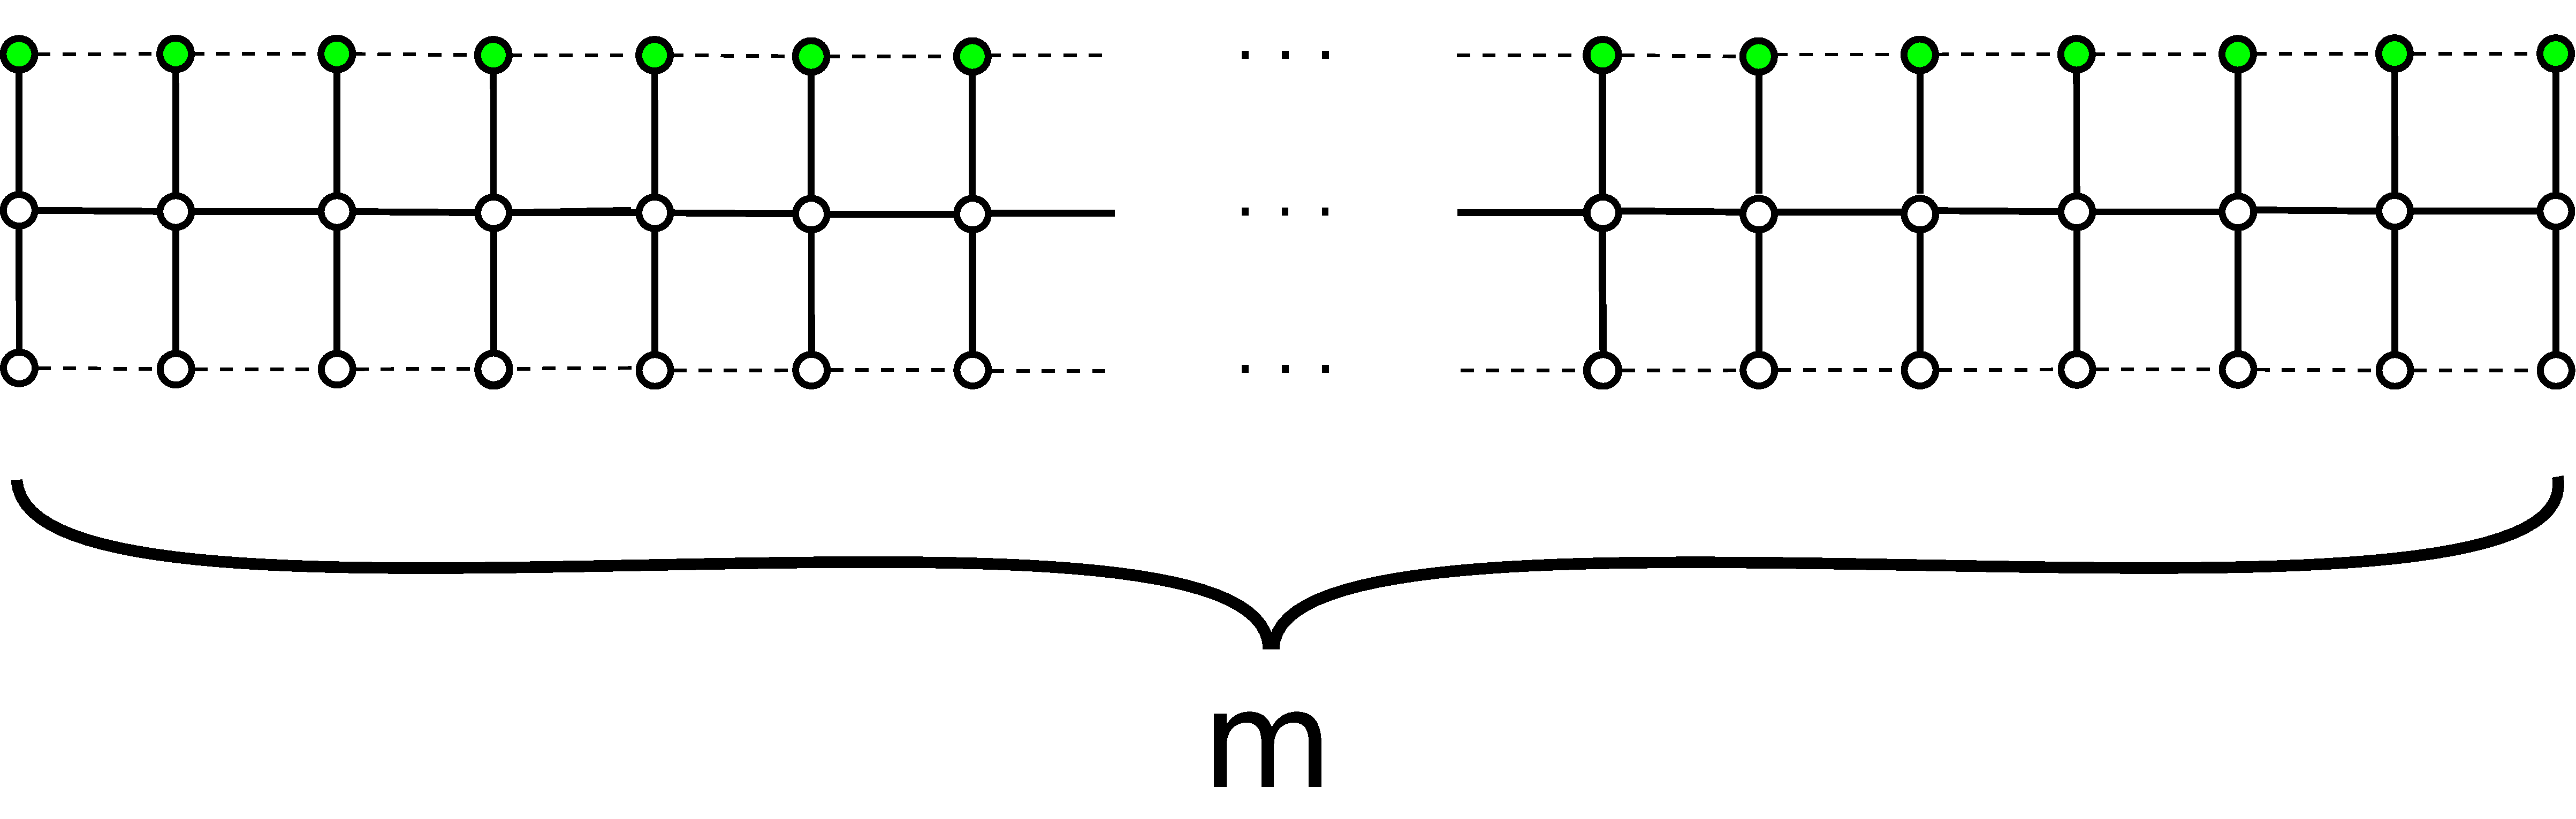
\includegraphics[width=420pt]{bilder/gitterzubaum.pdf}
   \caption{Beispiel für einen Teilgraphen mit größerer MD als der Graph selbst}
   \label{bild:Gitterbaum1}
\end{figure}
~ \linebreak
Der Gittergraph $G_{3,m}$ hat nach Tabelle \ref{tbl:Metrische Dimension einiger Graphklassen} metrische Dimension zwei. Werden $2m-2$ Kanten auf dem äußeren Kreis wie in Abbildung \ref{bild:Gitterbaum1} entfernt, so entsteht ein Baum $T_{3m}$ mit $2m$ Blättern. Die metrischen Dimension von diesem $T_{3m}$ ist $m$. Damit steigt die metrische Dimension von einem Graphen mit $n$ Knoten von zwei auf $\frac{n}{3}$.
\end{proof}
%%%%%%%%%%%%%%%%%%%%%%%%%%%%%%%%%%%%%%%%%%%%%%%%%%%%%%%%%%%%%%%%%%%%%%%%%%%%%%%%%%%%%%%%%%%%%%%%%%%%%%%%%%%%%%%%%%
%%%%%%%%%%%%%%%%%%%%%%%%%%%%%%%%%%%%%%%%%%%%%%%%%%%%%%%%%%%%%%%%%%%%%%%%%%%%%%%%%%%%%%%%%%%%%%%%%%%%%%%%%%%%%%%%%%
%%%%%%%%%%%%%%%%%%%%Löschen von Kanten vergößert MD%%%%%%%%%%%%%%%%%%%%%%%%%%%%%%%%%%%%%%%%%%%%%%%%%%%%%%%%%%%%%%%
%%%%%%%%%%%%%%%%%%%%%%%%%%%%%%%%%%%%%%%%%%%%%%%%%%%%%%%%%%%%%%%%%%%%%%%%%%%%%%%%%%%%%%%%%%%%%%%%%%%%%%%%%%%%%%%%%%
%%%%%%%%%%%%%%%%%%%%%%%%%%%%%%%%%%%%%%%%%%%%%%%%%%%%%%%%%%%%%%%%%%%%%%%%%%%%%%%%%%%%%%%%%%%%%%%%%%%%%%%%%%%%%%%%%%
\begin{lem}
Die metrische Dimension eines induzierten Teilgraphen ist nicht durch die metrische Dimension des ursprünglichen Graphen beschränkt. Durch das Entfernen von Knoten kann die metrische Dimension eines Graphen steigen.
\end{lem}
\vspace{-6mm}
%%%%%%%%%%%%%%%%%%%%%BEWEIS%%%%%%%%%%%%%%%%%%%%%%%%%%%%%%%%%%%%%%%%%%%%%%%%%%%%%%%%%%%%%%%%%%%%%%%%%%%%%%%%%%%%%
\begin{proof}[Beweis:]$\;$
\begin{figure}[h!]
		\centering 		 
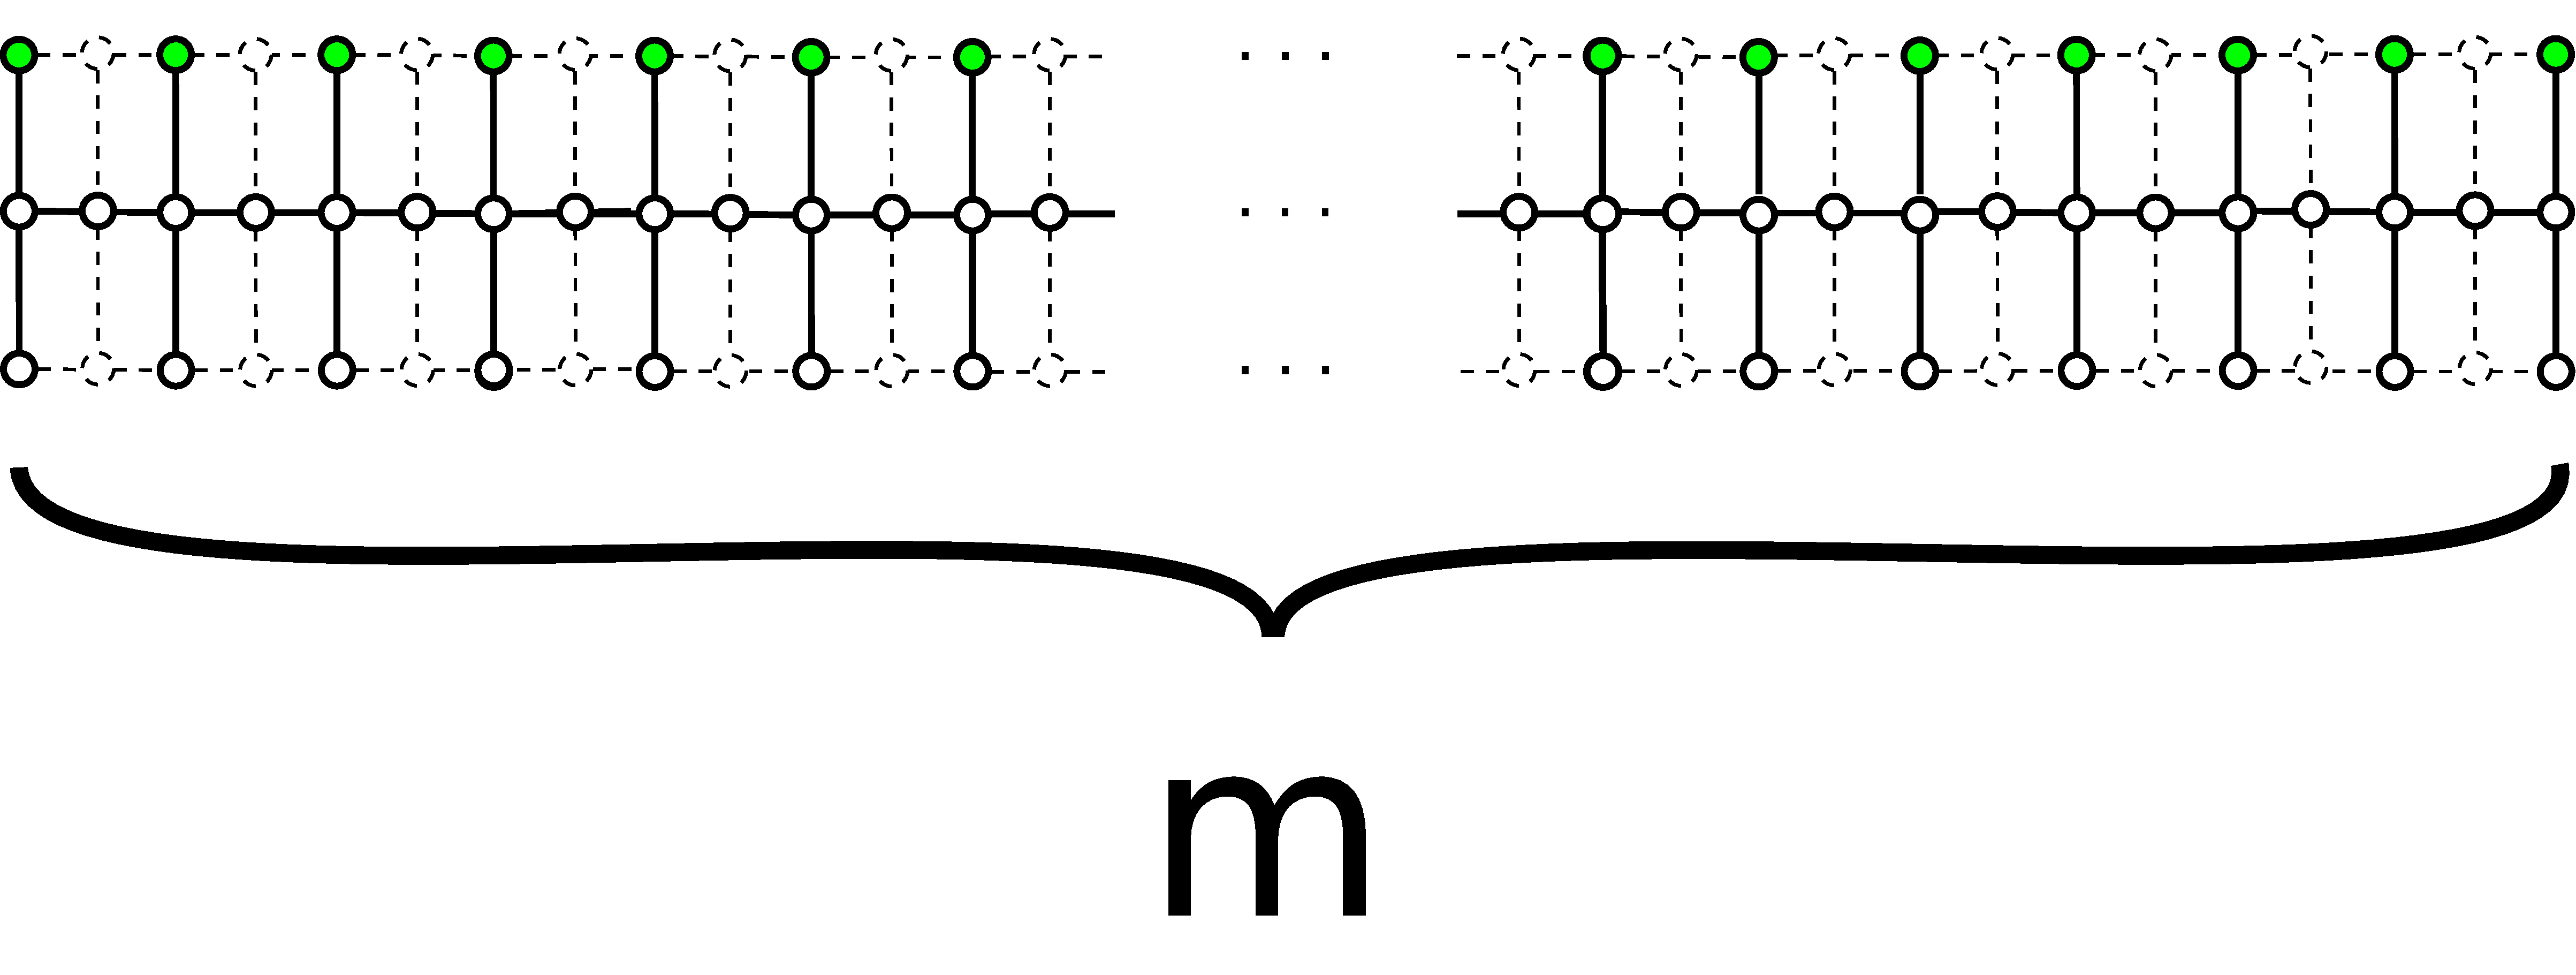
\includegraphics[width=420pt]{bilder/gitterzubaumlsch.pdf}
   \caption{Beispiel für einen induzierten TG mit größerer MD als der Graph selbst}
   \label{bild:Gitterbaum2}
  	 \end{figure}
~ \linebreak
Der Gittergraph $G_{3,2m-1}$ hat nach Tabelle \ref{tbl:Metrische Dimension einiger Graphklassen} metrische Dimension zwei. Entfernt man $2m-2$ Knoten, indem man alle äußeren Knoten behält und jeden zweiten Knoten auf dem äußeren Kreis entfernt, so entsteht ein Baum $T_{3m}$ wie in Abbildung \ref{bild:Gitterbaum2} mit der metrischen Dimension $m$. Damit steigt der Anteil von Knoten in der metrischen Basis von $6m-3:2$ auf $3m:m$.
\end{proof}
%\todo{Entfernen 1ner Kante, 1nem Knoten}

%%%%%%%%%%%%%%%%%%%%%%%%%%%%%%%%%%%%%%%%%%%%%%%%%%%%%%%%%%%%%%%%%%%%%%%%%%%%%%%%%%%%%%%%%%%%%%%%%%%%%%%%%%%%%%%%%%
%%%%%%%%%%%%%%%%%%%%%%%%%%%%%%%%%%%%%%%%%%%%%%%%%%%%%%%%%%%%%%%%%%%%%%%%%%%%%%%%%%%%%%%%%%%%%%%%%%%%%%%%%%%%%%%%%%
%%%%%%%%%%%%%%%%Zwei Teilgraphen mit je Element der MB trennen je 2 Knoten in unterschiedlichen TG %%%%%%%%%%%%%%%
%%%%%%%%%%%%%%%%%%%%%%%%%%%%%%%%%%%%%%%%%%%%%%%%%%%%%%%%%%%%%%%%%%%%%%%%%%%%%%%%%%%%%%%%%%%%%%%%%%%%%%%%%%%%%%%%%%
%%%%%%%%%%%%%%%%%%%%%%%%%%%%%%%%%%%%%%%%%%%%%%%%%%%%%%%%%%%%%%%%%%%%%%%%%%%%%%%%%%%%%%%%%%%%%%%%%%%%%%%%%%%%%%%%%%
\subsection{Allgemeine Eigenschaften}
\begin{lem}\cite{landmarks}
\label{dist}
Sei $G=(V,E)$ ein gegebener Graph. Seien $u,v$ und $w$ Knoten in $G$ und sei $\{u,v\}\in E$. Sei $d$ die Länge eines kürzesten Weges von $u$ zu $w$ in $G$. Dann ist die Länge eines kürzesten Weges von $v$ zu $w$ ein Element der Menge $\{d-1,d,d+1\}$.
\end{lem}
\begin{lem}
\cite{bases}
\label{einelementreichtnicht}
Sei ein beliebiger Graph $G=(V,E)$ gegeben. Der Graph $G'$ ensteht durch das Hinzufügen eines Knotens und das Verbinden von diesem Knoten mit genau einem anderen Knoten in $G$. Für die metrische Dimension von $G'$ gilt:
$$\beta(G)\leq \beta(G')\leq \beta(G)+1$$ 
\end{lem}
\begin{lem}
\label{wegtrennungsknoten}
\label{first_theorem}
Sei ein beliebiger Graph $G=(V,E)$ mit metrischer Basis $R=\{r_1, \ldots, r_k\}$ gegeben. Sei $(v,u) \in E$ eine Kante in $G$ und $v$ ein Trennungsknoten, welcher $G$ in zwei nichtleere Graphen $G'=(V',E')$ und $G"=(V",E")$ spaltet und sei der Knoten $u \in V"$. Dann gilt die folgende Aussage:\newline
Ist $r_i \notin G"$ für $1 \leq i \leq k$ dann ist $G"$ ein Weg.
\end{lem}
\begin{proof}[Beweis:]
Angenommen $G"$ ist kein Weg. Es gibt dann drei Fälle:
\begin{enumerate}
\item Angenommen der Knoten $v$ sei mit einem weiteren Knoten $w$, $w \neq u$, aus dem Graphen $G"$ verbunden. Da es keine Ankerknoten in $G"$ gibt haben die Knoten $u$ und $w$ die gleichen metrischen Koordinaten und sind nicht getrennt. Somit ist $u$ der einzige adjazente Knoten mit $v$ aus $G''$.
\item Angenommen $G"$ beinhaltet keinen Knoten mit Grad eins. Jeder Knoten hat mindestens zwei Nachbarn und damit auch der Knoten $u$. Da der Teilgraph keine Ankerknoten beinhaltet, haben die beiden Nachbaren von $u$ die gleichen metrischen Koordinaten und der Teilgraph ist nicht getrennt.
\item Der Knoten $u$ hat $deg(u)=1$ in dem Graphen $G"$. Der Knoten $v$ ist in dem Graphen $G$ nur mit dem Knoten $u$ aus Teilgraph $G"$ verbunden, dadurch hat der Knoten $u$ eine eindeutige Markierung. Es gibt einen Knoten $w$ mit $deg(w) \geq 3$, ansonsten wäre $G"$ ein Weg. Sei $p$ ein kürzester Weg von $u$ nach $w$ und $w_1$ und $w_2$ zwei Nachbarknoten von $w$, die nicht auf $p$ liegen. Da es keine weiteren trennenden Knoten in $G"$ gibt, haben die Knoten $w_1$ und $w_2$ dieselbe Markierung.   
\end{enumerate}
\vspace{-4mm}
\end{proof}
\begin{bem}
Vor allem folgt aus Lemma \ref{wegtrennungsknoten}, dass ein Teilgraph, welcher durch das Entfernen von einem Trennungsknoten entsteht und kein Weg ist, mindestens einen Ankerknoten beinhaltet.
\end{bem}
\begin{lem}
\label{second_theorem}
Gegeben sei ein Graph bestehend aus zwei nichtleeren Teilgraphen $G_R$ und $G_L$, welche durch genau eine Kante verbunden sind. Sofern jeder Teilgraph mind. ein Element aus der metrischen Basis beinhaltet, so ist jedes Knotenpaar $x,y$ mit der Eigenschaft $x \in G_R$ und $y \in G_L$ getrennt.
\end{lem}
%%%%%%%%%%%%%%%%%%%%%%%%%%%%%%%%%%%%%%%%%%%%%BEWEIS%%%%%%%%%%%%%%%%%%%%%%%%%%%%%%%%%%%%%%%%%%%%%%%%%%%%%%%%%%%%%%%
\vspace{-4mm}
\begin{proof}[Beweis:] ~
\vspace{-2mm}
\begin{figure}[h!]
		\centering 		 
  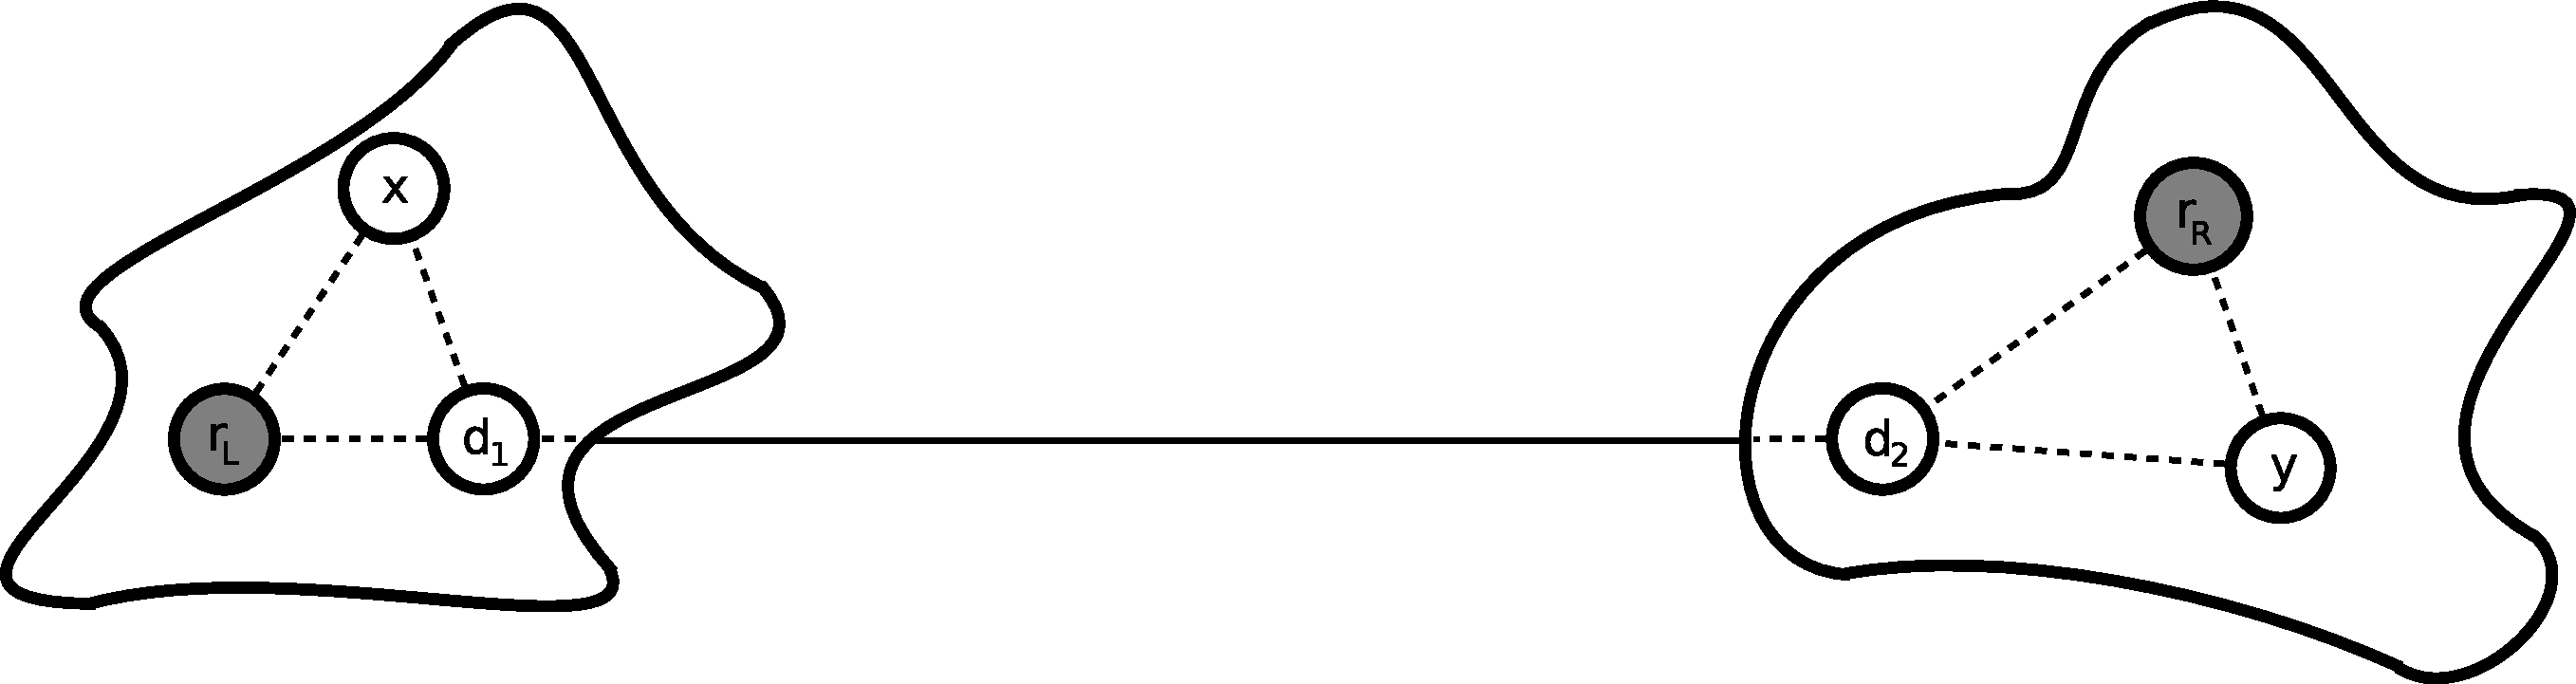
\includegraphics[width=340pt]{bilder/bew5.pdf}
	\caption{Ein Graph mit zwei über eine Kante verbundenen Teilgraphen mit jeweils einem Ankerknoten}
\vspace{-2mm}
  	 \end{figure}
  Angenommen es existiert ein nicht getrenntes Knotenpaar $x,y$.\\Sei $d_1$ der Bifurkator von $y,x,r_L$ und $d_2$ der Bifurkator von $x,y,r_R$. Dann gilt: $$dist(r_L,x) \leq dist(r_L,d_1)+ dist(d_1,x)\text{ und }dist(r_R,y) \leq dist(r_R,d_2)+ dist(d_2,y)$$ $$dist(r_L,y) > dist(r_L,d_1)+ dist(d_2,y)\text{ und }dist(r_R,x) > dist(r_R,d_2)+ dist(d_1,x)$$
  Da $x$ und $y$ nicht getrennt sind, gilt:
   $$dist(r_R,y) =dist(r_R,x),\: dist(r_L,x) = dist(r_L,y)$$ Dies kann eingesetzt und umgeformt werden zu dem folgenden Widerspruch:\begin{align*}
&\Rightarrow dist(r_L,d_1)+ dist(d_1,x) \geq dist(r_L,x) = dist(r_L,y)> dist(r_L,d_1)+ dist(d_2,y)\\
&\Leftrightarrow dist(r_L,d_1)+ dist(d_1,x) > dist(r_L,d_1)+ dist(d_2,y)\\
&\Leftrightarrow dist(d_1,x) >  dist(d_2,y)\\
&\Rightarrow dist(r_R,y) \leq dist(r_R,d_2)+ dist(d_2,y) < dist(r_R,d_2) + dist(d_1,x) < dist(r_R,x)\\
&\Leftrightarrow dist(r_R,y) < dist(r_R,x) = dist(r_R,y)\\&\Leftrightarrow dist(r_R,y) < dist(r_R,y) \lightning
\end{align*}  
   \vspace{-4mm}
  \end{proof}
  \begin{bem}
  \label{aussagetrennungsgraphen}
  Die Aussage lässt sich wie folgt verallgemeinern:\\
  Die beiden Teilgraphen $G_L$ und $G_R$ können nicht nur durch eine Kante oder durch einen Weg verbunden sein, sondern durch einen beliebigen Teilgraphen $G_M$, wenn es jeweils einen Trennungsknoten zwischen den Teilgraphen $G_L$ und $G_M$, und $G_R$ und $G_M$ gibt.
  \end{bem}
\begin{lem}
\label{Bifurnachbar}
Seien ein Graph $G=(V,E)$ und eine Menge $R \subset V$ mit $R=\{r_1, \ldots , r_n\}$, sowie außerwählte Knoten $v,x,y$ mit $dist_G(v,x)=dist_G(v,y)$ gegeben. Ist $v$ der Bifurkator von $r_i,x,y$ für $1 \leq i \leq n$ so ist $R$ keine metrische Basis von dem Graphen $G$.
\end{lem}
\begin{proof}[Beweis:]
Angenommen $R$ ist eine metrische Basis des Graphen $G$ und der Knoten $v$ besitze die Markierung $a_1/\ldots /a_n$. Sei die $dist_G(v,x)=b$. Da $v$ der Bifurkator ist liegt er auf einem kürzesten Weg und so ist die Markierung vom Knoten $x$ $a_1+b/\ldots /a_n+b$. Nach der Voraussetzung ist $dist_G(v,x)=dist_G(v,y)$, damit hat der Knoten $y$ die Markierung $a_1+b/\ldots /a_n+b$ und die Knoten $x$ und $y$ sind nicht getrennt. Dies ist ein Widerspruch zur Definition der metrischen Basis. $\lightning$
\end{proof}
~ \linebreak
\vspace{-12mm}
\begin{lem}
\label{bifur}
Sei ein beliebiger Graph $G=(V,E)$ gegeben. Wird ein Knotenpaar $u,v$ von einem Ankerknoten $r$ getrennt, so trennt jeder Knoten der den gleichen Bifurkator wie $r,\;u,\;v$ hat das Knotenpaar $u,v$.
\end{lem}
\begin{proof}[Beweis:]
Nach Definition liegt ein Bifurkator auf einem kürzesten Weg von $r$ zu $u$ und auf einem kürzesten Weg von $r$ zu $v$. Hätten die Knoten $u$ und $v$ die gleiche Entfernung zum Bifurkator oder zu jedem Knoten der auf dem eindeutigen Weg zwischen dem Bifurkator und dem Knoten $r$ liegt, so hätten sie die gleiche Entfernung zum Ankerknoten $r$ und wären nicht getrennt.
\end{proof}
\begin{lem}
\label{trennungsknoten}
Sei ein beliebiger Graph $G=(V,E)$ gegeben. Seien $G_1$ und $G_2$ zwei Teilgraphen von $G$ die durch einen Trennungsknoten $x$ verbunden sind. Jedes Knotenpaar aus $G_2$, welches von einem Ankernoten aus $G_1$ getrennt wird, wird auch von dem Knoten $x$ getrennt. Es gilt dasselbe für die Knotenpaare in $G_1$ und Ankerknoten in $G_2$.
\end{lem}
\begin{proof}[Beweis:]
Der Knoten $x$ ist ein Bifurkator zwischen jedem Knotenpaar in $G_2$ und jedem Ankerknoten in $G_1$ und umgekehrt. Damit folgt die Aussage nach Lemma \ref{bifur}.
\end{proof}
Betrachtet man nur den Teilgraphen $G_1 \cup \{x\}$ oder $G_2 \cup \{x\}$, so kann der Knoten $x$ lokal als Ankerknoten betrachtet werden. 
\begin{lem}
\label{keinknotenvonwegindermd}
Gegeben seien zwei Graphen $G_1=(V_1,E_1)$ und $G_2=(V_2,E_2)$ und zwei Knoten $u,v$ mit $u \in V_1$ und $v \in V_2$.
Der zusammenhängende Graph $G_n$ entsteht durch das Verbinden der Knoten $u$ und $v$ durch einen Weg der Länge $n \geq 1$. Die Knoten auf dem Weg werden als $p_i$ bezeichnet.\\
Für eine metrische Basis $R_k= \{ r_1, \ldots , r_k \}$ mit der Eigenschaft, dass es ein $r_i \in V_1$ und ein $r_j \in V_2$  mit $i \neq j$ gilt:
\[p_i \neq r_i \text{ für alle } i,j\]
\end{lem}
\begin{proof}[Beweis:]
Jeder Knoten auf dem Weg $p_i$ hat den gleichen Bifurkator für den Knoten $r_j$ und für jedes Knotenpaar in $G_1$ und das gleiche gilt für den Knoten $r_i$ und jedes Knotenpaar in $G_2$. Damit ist jeder Knoten auf dem Weg $p_i$ als Ankerknoten überflüssig.
\end{proof}
\begin{lem}
\label{nachbartrennungsknoten}
Sei ein beliebiger Graph $G=(V,E)$ gegeben. Seien $G_L$ und $G_R$ zwei Teilgraphen, die keine Wege sind, von $G$ die durch genau einen Trennungsknoten $v_s$ verbunden sind. Gibt es ein nicht getrenntes Knotenpaar $\{v_L,v_R\}$ mit der Eigenschaft, dass $v_L\in G_L$ und $v_R \in G_R$ und $v_L, v_R \notin \mathcal{N}(v_s)$.\newline
Dann ist das Knotenpaar $u_L,u_R \in \mathcal{N}(v_s)$, mit der Eigenschaften $u_L$ liegt auf dem kürzesten-Weg von $v_s$ zu $v_L$ und $u_R$ liegt auf dem kürzesten-Weg von $v_s$ zu $v_R$, nicht getrennt.
\end{lem}
\begin{proof}[Beweis:]~\newline
\vspace{-6mm}
\begin{figure}[!h]
\centering
\includegraphics[width=240pt]{bilder/nachbartrennungsknoten.pdf}
\end{figure}
~\linebreak
Da die Teilgraphen $G_L$ und $G_R$ keine Wege sind, beinhalten sie nach Lemma \ref{wegtrennungsknoten} jeweils mindestens einen Ankerknoten. Seien dies die Ankerknoten $r_R \in G_R$ und $r_L \in G_L$. Angenommen die Knoten $u_L,u_R$ mit den obigen Eigenschaften seien getrennt, also: $$dist(r_L,u_R)\neq dist(r_L,u_L)\; [1]\;\;\; \text{oder}\;\;\; dist(r_R,u_R)\neq dist(r_R,u_L)\; [2].$$
  Da die Knoten $v_L, v_R \notin \mathcal{N}(v_s)$ gilt: $$dist(v_s,v_R),dist(v_s,v_L)\geq 2.$$ Die Knoten $v_L$ und $v_R$ sind nicht getrennt, also gilt: $$dist(r_L,v_R)=dist(r_L,v_L)\;\;\; \text{und}\;\;\; dist(r_R,v_R)=dist(r_R,v_L).$$ Da $u_L,u_R \in \mathcal{N}(v_s)$ gilt $$dist(r_L,u_R)=dist(r_L,v_s)+1\;\;\; \text{und}\;\;\;dist(r_R,u_L)=dist(r_R,v_s)+1.$$   
Die metrischen Koordinaten von $u_L$ und $u_R$ wären gleich $dist(r_R,v_s)+1/dist(r_L,v_s)+1$, außer ein Weg von einem Ankerknoten über einen der Knoten $v_L$ und $v_R$ ist kürzer. Daraus folgt: $$dist(r_L,v_s)+dist(r_L,v_L)+dist(v_L,v_s)-1< dist(r_L,v_s)+1\;[1]$$ \begin{center} oder \vspace{-2mm} \end{center}
$$dist(r_R,v_s)+dist(r_R,v_R)+dist(v_R,v_s)-1< dist(r_R,v_s)+1\;[2]$$ 

Für Fall 1 gilt:
\begin{align*}
&\;\;\;\;\;\;dist(r_R,v_s)+dist(r_R,v_R)+dist(v_R,v_s)-1< dist(r_R,v_s)+1\\
&\Leftrightarrow dist(r_R,v_R)+dist(v_R,v_s)-1< 1\\
&\Leftrightarrow dist(r_R,v_L)+dist(v_R,v_s)-1< 1\\
&\Leftrightarrow dist(r_R,v_s)+ dist(v_s,v_L)+dist(v_R,v_s)-1 < 1\\
&\Leftrightarrow dist(r_R,v_s)+dist(v_s,v_L)+dist(v_R,v_s)< 2\\
&\Leftrightarrow  4 \leq dist(r_R,v_s) +4 \leq dist(r_R,v_s)+dist(v_s,v_L)+dist(v_R,v_s)< 2 \lightning
\end{align*}

Der Beweis für Fall 2 folgt analog. 
  \end{proof}
Es kann gezeigt werden, dass die Aussage auch für Teilgraphen ohne Ankerknoten gilt.
\begin{lem}
\label{nachbartrennungsknoten2}
Sei ein beliebiger Graph $G=(V,E)$ gegeben. Seien $G_L$, $G_R$, die keine Wege sind, und ein Weg $p$ drei Teilgraphen von $G$ die durch genau einen Trennungsknoten $v_s$ verbunden sind. Gibt es ein nicht getrenntes Knotenpaar $\{v_L,v_R\}$ mit der Eigenschaft, dass $v_L\in p$ und $v_R \in G_R$ und $v_L, v_R \notin \mathcal{N}(v_s)$, dann ist das Knotenpaar $u_L,u_R \in \mathcal{N}(v_s)$ mit der Eigenschaft, dass $u_L$ auf dem kürzesten-Weg von $v_s$ zu $v_L$ und $u_R$ auf dem kürzesten-Weg von $v_s$ zu $v_R$ liegt, nicht getrennt.
\end{lem}
\par
\begin{proof}[Beweis:] Angenommen die Knoten $u_L,u_R$ mit den obigen Eigenschaften seien getrennt.
\begin{floatingfigure}[r]{200pt}
\centering
\includegraphics[width=170pt]{bilder/nachbartrennungsknoten2.pdf}
\end{floatingfigure}
Nur Knoten aus dem Teilgraphen $G_R$ können das Knotenpaar trennen. Angenommen, es gilt: $$dist(r_R,u_R)\neq dist(r_R,u_L)$$
\newline
Da die Knoten $v_L, v_R \notin \mathcal{N}(v_s)$ und nicht getrennt sind, gilt: $$dist(v_s,v_R),dist(v_s,v_L)\geq 2,\;\;\; dist(r_R,v_R)=dist(r_R,v_L)$$ 
Aus $$dist(r_L,v_R)=dist(r_L,v_L) \text{ folgt }dist(v_s,v_R)=dist(v_s,v_L)$$\\
Nach Lemma \ref{dist} gilt: $$dist(r_R,u_R)\in \{dist(r_R,v_s)-1,\; dist(r_R,v_s),\;dist(r_R,v_s)+1\}$$
Da $u_L,\;u_R \in \mathcal{N}(v_s)$ und $u_R$ auf dem kürzesten Weg zu $v_R$ von $v_s$ ist, gilt: $$dist(r_R,u_L)=dist(r_R,v_s)+1\text{ und }dist(v_R,v_s)=dist(v_R,u_R)+1$$
Also sind $$dist(r_R,u_R)\neq dist(r_R,u_L)\text{ wenn }dist(r_R,u_R)<dist(r_R,v_s)+1=dist(r_R,u_L)$$
Dies ist nur der Fall wenn: $$dist(r_R,u_R)\in \{dist(r_R,v_s)-1,\; dist(r_R,v_s)\}$$
Daraus folgt, dass:
\begin{align*}
&\;\;\;\;\;\;dist(r_R,v_s)+dist(v_s,v_L)=dist(r_R,v_L)=dist(r_R,v_R)\\
&\Leftrightarrow  dist(r_R,v_s)+dist(v_s,v_L)=dist(r_R,v_R) \leq dist(r_R,u_R)+dist(u_R,v_R)\\
&\Leftrightarrow  dist(r_R,v_s)+dist(v_s,v_L)=dist(r_R,v_R)< dist(v_R,v_s)+dist(u_R,v_R)\\
&\Leftrightarrow  dist(r_R,v_s)+dist(v_s,v_L)< dist(v_R,v_s)+dist(r_R,v_s)\\
&\Leftrightarrow  dist(r_R,v_s)<dist(r_R,v_s)\lightning
\end{align*}
\end{proof}
\par
%%%%%%%%%%%%%%%%%%%%%%%%%%%%%%%%%%%%%%%%%%%%%%%%%%%%%%%%%%%%%%%%%%%%%%%%%%%%%%%%%%%%%%%%%%%%%%%%%%%%%%%%%%%%%%%%%%
%%%%%%%%%%%%%%%%%%%%%%%%%%%%%%%%%%%%%%%%%%%%%%%%%%%%%%%%%%%%%%%%%%%%%%%%%%%%%%%%%%%%%%%%%%%%%%%%%%%%%%%%%%%%%%%%%%
%%%%%%%%%%%%%%%%%%%%Knotenkontraktion von Trennungsknoten vergrößert nicht%%%%%%%%%%%%%%%%%%%%%%%%%%%%%%%%%%%%%%%%
%%%%%%%%%%%%%%%%%%%%%%%%%%%%%%%%%%%%%%%%%%%%%%%%%%%%%%%%%%%%%%%%%%%%%%%%%%%%%%%%%%%%%%%%%%%%%%%%%%%%%%%%%%%%%%%%%%
%%%%%%%%%%%%%%%%%%%%%%%%%%%%%%%%%%%%%%%%%%%%%%%%%%%%%%%%%%%%%%%%%%%%%%%%%%%%%%%%%%%%%%%%%%%%%%%%%%%%%%%%%%%%%%%%%%
\subsection{Der Einfluß von Knotenkontraktion von Trennungsknoten vom Grad zwei auf die metrische Dimension}
Gegeben seien zwei Graphen $G_1=(V_1,E_1)$ und $G_2=(V_2,E_2)$ und zwei Knoten $u,v$ mit $u \in V_1$ und $v\in V_2$.
Der zusammenhängende Graph $G$ entsteht durch das Verbinden der Knoten $u$ und $v$ durch einen Weg $p$ der Länge $n \geq 1$. Bei einer metrischen Basis $R_k$ mit $k \geq 2$ befindet sich mindestens ein Ankerknoten in jedem Teilgraph $G_1$ und $G_2$. Nach Lemma \ref{keinknotenvonwegindermd} können nur Knoten aus den Teilgraphen $G_1$ und $G_2$ Ankerknoten sein. In diesem Abschnitt werden nur solche Graphen $G$ betrachtet.
\begin{lem}
\label{lem2}
\label{sepvertex}
Durch die Kontraktion von Trennungsknoten vom Grad zwei kann die metrische Dimension eines Graphen $G$ nicht vergrößert werden.
\end{lem}
%%%%%%%%%%%%%%%%%%%%%%%%%%%%%%%%%%%BEWEIS%%%%%%%%%%%%%%%%%%%%%%%%%%%%%%%%%%%%%%%%%%%%%%%%%%%%%%%%%%%%%%%%%%%%%%%%%
\begin{proof}[Beweis:]
Sei ein Graph $G$ mit einer metrischen Basis $R_k$ und einem Trennungsknoten $v_s$ mit $deg(v_s)=2$ gegeben. Die zwei Teilgraphen welche durch das Entfernen von $v_s$ entstehen bezeichne man als $G_R$ und $G_L$.
\begin{figure}[ht]
\centering
\includegraphics*[width = 250pt]{bilder/proof4,2.pdf}
\caption{Ein Graph mit einem Trennungknoten vom Grad zwei}
\end{figure}
\newline Der Graph $G'$ resultiert durch die Kontraktion von $v_s$ mit einem beliebigen Nachbarn. Da der Knoten $v_s$ auf dem Weg $p$ liegt ist er nach Voraussetzung kein Ankerknoten.\newline
Angenommen die metrische Dimension in $G'$ ist größer als in $G$, dann existiert ein\\Knotenpaar $x,y$, welches in $G$ getrennt wird, aber nicht in $G'$.\\Also gibt es mindestens einen Knoten in der metrischen Basis $R_K$ vom Graphen $G$, welcher $x,y$ trennt. Sei dies der Knoten $r_k$. Dieser Knoten trennt $x,y$ nicht in dem Graphen $G'$. 
Betrachte nun die Fälle einzeln:
\begin{itemize}
\item Falls alle drei Knoten in dem gleichen Teilgraphen sind, so ist $v_s$ in keinem kürzesten Weg enthalten und $x,y$ bleiben getrennt, sofern sie zuvor getrennt waren.
\item Sind die Knoten $x,y$ in einem Teilgraphen und $r_k$ in dem Anderen, so schrumpft die Distanz des kürzesten Weges von $r_k$ zu $x$ und zu $y$ um genau eins und bleibt dabei unterschiedlich auch in $G'$.
\item Die Knoten $x$ und $y$ sind in unterschiedlichen Teilgraphen. Nach Annahme beinhaltet jeder der Teilgraphen $G_R$ und $G_L$ mind. ein Element aus der metrischen Basis. Der Widerspruch folgt unmittelbar aus Lemma \ref{first_theorem}.
\end{itemize}
\end{proof}
%%%%%%%%%%%%%%%%%%%%%%%%%%%%%%%%%%%%%%%%%%%%%%%%%%%%%%%%%%%%%%%%%%%%%%%%%%%%%%%%%%%%%%%%%%%%%%%%%%%%%%%%%%%%%%%%%%
%%%%%%%%%%%%%%%%%%%%%%%%%%%%%%%%%%%%%%%%%%%%%%%%%%%%%%%%%%%%%%%%%%%%%%%%%%%%%%%%%%%%%%%%%%%%%%%%%%%%%%%%%%%%%%%%%%
%%%%%%%%%%%%%%%%%%%%Knotenkontraktion von Trennungsknoten verkleinert nicht(SF)%%%%%%%%%%%%%%%%%%%%%%%%%%%%%%%%%%%
%%%%%%%%%%%%%%%%%%%%%%%%%%%%%%%%%%%%%%%%%%%%%%%%%%%%%%%%%%%%%%%%%%%%%%%%%%%%%%%%%%%%%%%%%%%%%%%%%%%%%%%%%%%%%%%%%%
%%%%%%%%%%%%%%%%%%%%%%%%%%%%%%%%%%%%%%%%%%%%%%%%%%%%%%%%%%%%%%%%%%%%%%%%%%%%%%%%%%%%%%%%%%%%%%%%%%%%%%%%%%%%%%%%%%
\begin{lem}
\label{sepvertex2}
Durch die Kontraktion von Kanten, sofern ein inzidenter Knoten ein Trennungsknoten vom Grad zwei ist, kann die metrische Dimension eines Graphen $G$ nicht verkleinert werden.
\end{lem}
%%%%%%%%%%%%%%%%%%%%%%%%%%%%%%%%%%%BEWEIS%%%%%%%%%%%%%%%%%%%%%%%%%%%%%%%%%%%%%%%%%%%%%%%%%%%%%%%%%%%%%%%%%%%%%%%%%
\begin{proof}[Beweis:]
Sei ein Graph $G$ mit einer metrischen Basis $R_k$ und einem Trennungsknoten $v_s$ mit $deg(v_s)=2$ gegeben. Die zwei Teilgraphen welche durch das Entfernen von $v_s$ entstehen bezeichne man als $G_R$ und $G_L$.
Der Graph $G'$ resultiert durch die Kontraktion der Kante an $v_s$ und einem beliebigen Nachbarn. Da der Knoten $v_s$ auf dem Weg $p$ liegt ist er nach Voraussetzung kein Ankerknoten.\newline
Angenommen die metrische Dimension in $G'$ ist kleiner als in $G$, dann existiert ein\\Knotenpaar $x,y$, welches in $G'$ getrennt wird, aber nicht in $G$.\\Also gibt es mindestens einen Knoten in der metrischen Basis $R_K$ des Graphens $G'$, welcher $x,y$ trennt. Sei dies der Knoten $r_k$. Dieser Knoten trennt $x,y$ nicht in dem Graphen $G$. 
Betrachte nun die Fälle einzeln:
\begin{itemize}
\item Falls alle drei Knoten in dem gleichen Teilgraphen sind, so ist $v_s$ in keinem kürzesten Weg enthalten und $x,y$ getrennt, sofern sie zuvor getrennt waren.
\item Sind die Knoten $x,y$ in einem Teilgraphen und $r_k$ in dem Anderen, so schrumpft die Distanz des kürzesten Weges von $r_k$ zu $x$ und zu $y$ um genau eins und bleibt dabei unterschiedlich auch in $G'$.
\item Sind die Knoten $x$ und $y$ in unterschiedlichen Teilgraphen, so beinhaltet jeder der Teilgraphen $G_R$ und $G_L$ nach Annahme mind. ein Element aus der metrischen Basis. Der Widerspruch folgt unmittelbar aus dem Lemma \ref{first_theorem}.
\vspace{-5mm}
\end{itemize}
\end{proof}
\begin{bem}
Nach den Lemmata \ref{sepvertex} und \ref{sepvertex2} folgt, dass neben der Kontraktion von Kanten die Erweiterung von Knoten auf einem Weg $p$ zwischen zwei Teilgraphen keinen Einfluß auf die metrische Dimension hat, sofern die Teilgraphen Ankerknoten besitzen. Insbesondere folgt für die Bestimmung der metrischen Dimension, dass Wege zwischen Teilgraphen, die Ankerknoten besitzen, zu einer Kante kontrahiert werden können, ohne dabei die metrische Dimension des Graphen zu verändern.
\end{bem}
\begin{lem}
Ist in einem Teilgraphen kein Ankerknoten enthalten, so kann durch die Kontraktion Kanten, sofern ein inzidenter Knoten ein Trennungsknoten vom Grad zwei ist, die metrische Dimension eines Graphen verkleinert werden.
\end{lem}
\begin{proof}[Beweis:] ~ \newline
\vspace{-7mm}
\begin{figure}[!h]
\centering
\includegraphics[width=290pt]{bilder/gegbspsepvertex.pdf}
\caption{Graph $G$ (rechts) und Graph $G'$ nach der Kontraktion der Kante an blauem Trennungsknoten (links)}
\end{figure} 
\vspace{-8mm}
~\linebreak
\end{proof}
Im Allgemeinen kann keine Kontraktion oder Erweiterung bei Wegen vorgenommen werden, aber es gibt Spezialfälle bei denen die metrische Dimension dadurch nicht verändert wird.
\begin{lem}
Bei Bäumen können ohne Auswirkungen auf die metrische Dimension Kanten, sofern ein inzidenter Knoten den Grad zwei hat, kontrahiert werden oder mit Knoten kann ohne Auswirkungen auf die metrische Dimension erweitert werden.
\end{lem}
\begin{proof}[Beweis:]
Der Algorithmus aus Lemma \ref{baum} zur Berechnung der metrischen Dimension beachtet nur die Anzahl der einfachen Wege an jedem Knoten mit mindestens Grad drei. Die Länge der Wege kann ohne Auswirkungen auf die metrische Dimension des Graphen beliebig verändert werden.
\end{proof}
\begin{lem}
\label{sonneerweiterung}
Bestehe ein Graph $G$ aus einem Kreis mit jeweils einem einfachen Weg an jedem Kreisknoten (Sonne aus Definition \ref{sun}). Auf jeder Kante auf dem Weg kann mit Knoten vom Grad zwei erweitert werden und Knoten von Grad zwei können ohne Auswirkungen auf die metrische Dimension kontrahiert werden.
\end{lem}

\begin{proof}[Beweis:]
Sei ein getrennter Kreis $G=(V,E)$ mit Wegen der Länge eins und seine metrische Basis $R$ gegeben. Eine Kante auf einem Weg an Knoten $v_k$ wird um einen Knoten erweitert, so dass sich die metrischen Koordinaten von Knoten $v$, welcher kein Ankerknoten ist, um eins erhöhen. Sei $a+2/b+2$ für einen ungeraden Kreis und $a+2/b+2/c+2$ für einen geraden Kreis die neuen metrischen Koordinaten von $v$. Angenommen, es gibt einen Knoten $u$ in dem Graphen $G$ mit den gleichen metrischen Koordinaten.
\begin{enumerate}
\item Der Knoten $v_k$ hat die metrischen Koordinaten $a/b$ oder $a/b/c$. Sofern es einen anderen Knoten $v'$ als $v$ gibt mit der Distanz zwei zu dem Knoten $v_k$ und den gleichen metrischen Koordinaten wie $v$, so gibt es auch einen Knoten zwischen den Knoten $v'$ und $v$ mit den metrischen Koordinaten $a+1/b+1$ oder $a+1/b+1/c+1$. Dieser Knoten hat die gleichen metrischen Koordinaten wie der Knoten $v$ vor der Erweiterung. Dadurch hätte der ursprüngliche Graph nicht getrennt sein können.
\item Angenommen, es gibt einen Knoten $v'$ als $v$ mit der Distanz $2a+2$ zu dem Knoten $v_k$ und den gleichen metrischen Koordinaten wie $v$.
\begin{itemize}
\item Der Knoten $v'$ liegt auf dem Kreis. Wenn der kürzeste Weg über alle Ankerknoten gleich ist, tritt Fall 1 auf.
\begin{itemize}
\item Ist der Kreis ungerade, so ist die metrische Koordinate ist $b-b+2n+1-2a-2=2(n-a)-1$. Dieser Wert kann bei beliebiger Wahl von $a,b,n \in \mathbb{N}$ nicht gerade sein und damit gilt insbesondere: $2(n-a)-1\neq 2b+2$. 
\item Ist der Kreis gerade, so können die metrischen Koordinaten gleich sein, wenn zwei Ankerknoten im gleichen Strahl sind. Ist das der Fall, so wäre auch der ursprüngliche Graph nicht getrennt. Ausgenommen von diesem Strahl werden dieselben Knotenpaare von beide Ankerknoten getrennt, und nach Lemma \ref{mdgr2} reichen zwei Ankerknoten nicht aus um einen geraden Sonnengraphen zu trennen. Sind alle Knoten in unterschiedlichen Wegen, so kann es keine zwei Knoten mit einer Distanz $\geq \frac{n}{2}$ geben, so dass alle drei Markierungen gleich sind.
\end{itemize}
\item Der Knoten $v'$ ist ein Blatt, so geht der Beweis analog.
%\begin{itemize}
%\item Dann gibt es einen Strahlursprung $v'_k$ mit der Distanz eins zu dem Knoten $v'$ und mit der Distanz $2a+1$ zu dem Knoten $v_k$. Angenommen die Ankerknoten haben keinen gemeinsamen Bifurkator, dann hat $v'$ die metrische Koordinate $b-b+2n-2a-1=2(n-a)$. Dieser Wert ist für alle $a,b,n \in \mathbb{N}$ gerade und damit auch $2(n-a)\neq 2b+1$.
%\item In einem geraden Sonnengraphen kann es keine zwei Knoten geben, so dass die Distanz von drei Ankerknoten zu diesen beiden Knoten gleich ist. Ausgenommen mindestens zwei Knoten liegen aus einem Strahl.
%\end{itemize}
\end{itemize}
\end{enumerate}
\end{proof}
%%%%%%%%%%%%%%%%%%%%%%%%%%%%%%%%%%%%%%%%%%%%%%%%%%%%%%%%%%%%%%%%%%%%%%%%%%%%%%%%%%%%%%%%%%%%%%%%%%%%%%%%%%%%%%%%
%%%%%%%%%%%%%%%%%%%%%%%%%%%%%%%%%%%%%%%%%%%%%%%%%%%%%%%%%%%%%%%%%%%%%%%%%%%%%%%%%%%%%%%%%%%%%%%%%%%%%%%%%%%%%%%%
%%%%%%%%%%%%%%%%%%%%%%%%%%%%%%%%%%%%%%%%%%%%%%%%%%%%%%%%%%%%%%%%%%%%%%%%%%%%%%%%%%%%%%%%%%%%%%%%%%%%%%%%%%%%%%%%
\chapter{Metrische Dimension von kreisähnlichen Graphklassen}
\vspace{-5mm}
In diesem Kapitel geht es um Erweiterungen von bekannten Graphklassen. Als erstes werden der Sonnengraph mit der unvollständigen Variante und dannach der Freundschaftsgraph und seine Verallgemeinerung untersucht.
Von den verallgemeinerten Freundschaftsgraphen und beiden Sonnengraphen wird die metrische Dimension bestimmt unter der Voraussetzung, dass bestimmte Ankerknoten fest vorgegeben sind. Die Resultate werden beim Algorithmus zur Bestimmung der metrischen Dimension von Kaktusgraphen in Kapitel \ref{kapkaktus} und beim Beweis der metrischen Dimension der $C_j$-Bäume in Kapitel \ref{kapcjbaume} benötigt.
\vspace{-6mm}
%%%%%%%%%%%%%%%%%%%%%%%%%%%%%%%%%%%%%%%%%%%%%%%%%%%%%%%%%%%%%%%%%%%%%%%%%%%%%%%%%%%%%%%%%%%%%%%%%%%%%%%%%%%%%%%%
\section{Metrische Dimension der Sonnengraphen $S_{n,k}$}
\label{chap_sonne}
In der Arbeit "On k-dimensional graphs and their bases" \cite{bases} wird die metrische Dimension des Corona Produktes von Kreisen $C_n$ und Wegen $P_1$ betrachtet. Diese Graphen sind in der Literatur auch unter dem Namen "sunlet" \cite{sunwebsite} bekannt. In diesem Kapitel wird gezeigt, dass ihr Resultat sich auf Wege beliebiger Länge übertragen lässt. Außerdem werden ebenfalls Teilgraphen der Sonnengraphen betrachtet, die unvollständigen Sonnengraphen. Beide Graphklassen sind sehr wichtig für den Algorithmus in Kapitel \ref{kapkaktus}.

\begin{defi}{\textbf{(Sonnengraph $S_{n}$)}}
\label{sun}
\begin{floatingfigure}[r]{180pt}
{\centering
\hspace*{0.1cm}
 		 \includegraphics[width=178pt]{bilder/sonne4.pdf}}
   \caption{Sonnengraph $S_{12,3}$}
   \label{bild:sonnengraph}
\end{floatingfigure}
Sei ein Kreis $C_n$ für $n \geq 3$ mit der Knotenmenge $|V|=\{ c_1, \ldots , c_n \}$ und $n$ Weggraphen $P_{k-1}$ für $k \geq 2$ gegeben. Die Knoten mit Grad eins auf dem $i-$ten Weg werden als $v_{i,1}$ und $v_{i,k-1}$ bezeichnet. Durch das Hinzufügen von $n$ neuen Kanten der Form $\{v_{i,1},c_i\}$ für $1 \leq i \leq n$ ensteht der zusammenhängende Sonnengraph $S_{n,k}$.\\
Alle als $v_{i,k-1}$ bezeichneten Knoten werden Endknoten genannt, als $c_i$ bezeichnete Knoten werden Ursprungsknoten genannt und eine Knotenmenge mit den Knoten $\{c_i,v_{i,1}, \ldots ,v_{i,k-1}\}$ für $1 \leq i \leq n$ als Strahl. (vgl. Abbildung \ref{bild:sonnengraph})\\
Für $n=1$ ist der Graph der Sterngraph aus Definition \ref{defstern}. Als Sonnengraph $S_n$ bezeichne man einen Graphen mit $n$ Strahlen beliebiger Länge $i$ mit $i \geq 1$. Ist $n=2m+1$ so nennt man den Sonnengraphen ungerade, ist $n=2m+2$ mit $m \in \mathbb{N}^+$ so bezeichnet man den Sonnengraphen als gerade.
\par
\end{defi}
\newpage
%\begin{bem}
%Nach Satz \ref{sepvertex} können beliebige Wege $P_i$ mit $i\geq 2$ bei der Berechnung der metrischen Dimension als $P_2$ aufgefasst werden. Also gilt: $$md(S_{n,2})=md(S_{n,3})= \ldots =md(S_{n,k})=md(S_{n})$$
%Im folgenden wird der Graph $S_{n,2}$ repräsentativ für $S_{n,k}$ betrachtet.
%\end{bem}
\begin{lem}\cite{bases}
\label{sun1}
Für die metrische Dimension eines Sonnengraphen $S_{n,1}$ gilt:
\begin{equation}
   \beta(S_{n,1})=
   \begin{cases}
     2 & \text{f\"ur } n = 4 \text{ oder } n = 2j+1 \text{ f\"ur } j \in \mathbb{N} \\
     3 & \text{f\"ur } n = 2j+4 \text{ f\"ur } j \in \mathbb{N} 
   \end{cases}
\end{equation}
\end{lem}
\begin{lem}
\label{knotenimstrahl}
Es gibt pro Strahl nur einen Ankerknoten. Das Vorziehen eines Endknotens gegenüber einem Strahlurprung als Ankerknoten im gleichen Strahl bringt nur Vorteile.
\end{lem}
\begin{proof}[Beweis:]
Angenommen der Endknoten eines Strahls ist ein Ankerknoten $r$. Der Bifurkator zwischen jedem Knoten auf dem Strahl und einem beliebigen Knotenpaar im restlichen Graphen ist der Strahlursprung. Der Strahlursprung ist ebenfalls der Bifurkator für den Ankerknoten und jedem Knotenpaar im Graphen außerhalb des Strahls. Nach Lemma \ref{bifur} ist jeder Knoten auf dem Strahl damit kein zusätzlicher Ankerknoten. Jeder Knoten auf dem Strahl ist im gesamten Graphen getrennt, da er durch einen Weg eine eindeutige Distanz zu dem Ankerknoten $r$ hat.\begin{figure}[h!]
		\centering
 		 \includegraphics[width=300pt]{bilder/bspsonne4.pdf}
   \caption{$S_4$ mit zwei Ankerknoten unterschiedlich positioniert}
   \label{s4}
   \end{figure}
Nimmt man in einem Strahl den Strahlursprung an Stelle des Endknotens so kann ein getrennter Graph nicht nicht mehr getrennt sein (vgl. dazu Abbildung \ref{s4}).
\end{proof}
%Es werden nur noch metrische Basen betrachtet mit maximal einem Ankernoten in einem Strahl. Das Auswirkungen von Lemma \ref{sonneerweiterung}, dass für die Bestimmung der metrischen Dimension einer Sonne $S_n$ einfach die metrische Dimension einer Sonne $S_{n,1}$ bestimmt werden kann. 
\begin{bem}
Es werden nur noch metrische Basen mit maximal einem Ankernoten in einem Strahl betrachtet. O.B.d.A. ist der Endknoten des Strahls der Ankerknoten. Außerdem gilt nach Lemma \ref{sonneerweiterung} für die metrische Dimension von Sonnengraphen: $$\beta(S_{n,1})=\beta(S_{n,k})=\beta(S_n)$$
Dadurch wird bei der weiteren Berechnung nur der Sonnengraph $S_{n,1}$ beachtet, da sich die Ergebnisse auf jeden beliebigen Sonnengraph übertragen lassen. 
\end{bem}
\begin{lem}
\label{mdgr2}
Die metrische Dimension eines Sonnengraphen $S_{n}$ mit $n = 2j+4$ für $j \in \mathbb{N}^+$ ist größer als zwei. 
\end{lem}
%\begin{figure}[h!]
%\begin{minipage}[hbt]{7cm}
%	\centering
%	\includegraphics[width=170pt]{bilder/sonne4k.pdf}  
 %  \caption{Der Sonnengraph $S_{4,2}$}  
	%\label{Bild1}
%\end{minipage}
%\hfill
%\begin{minipage}[hbt]{7cm}%
%	\centering
%	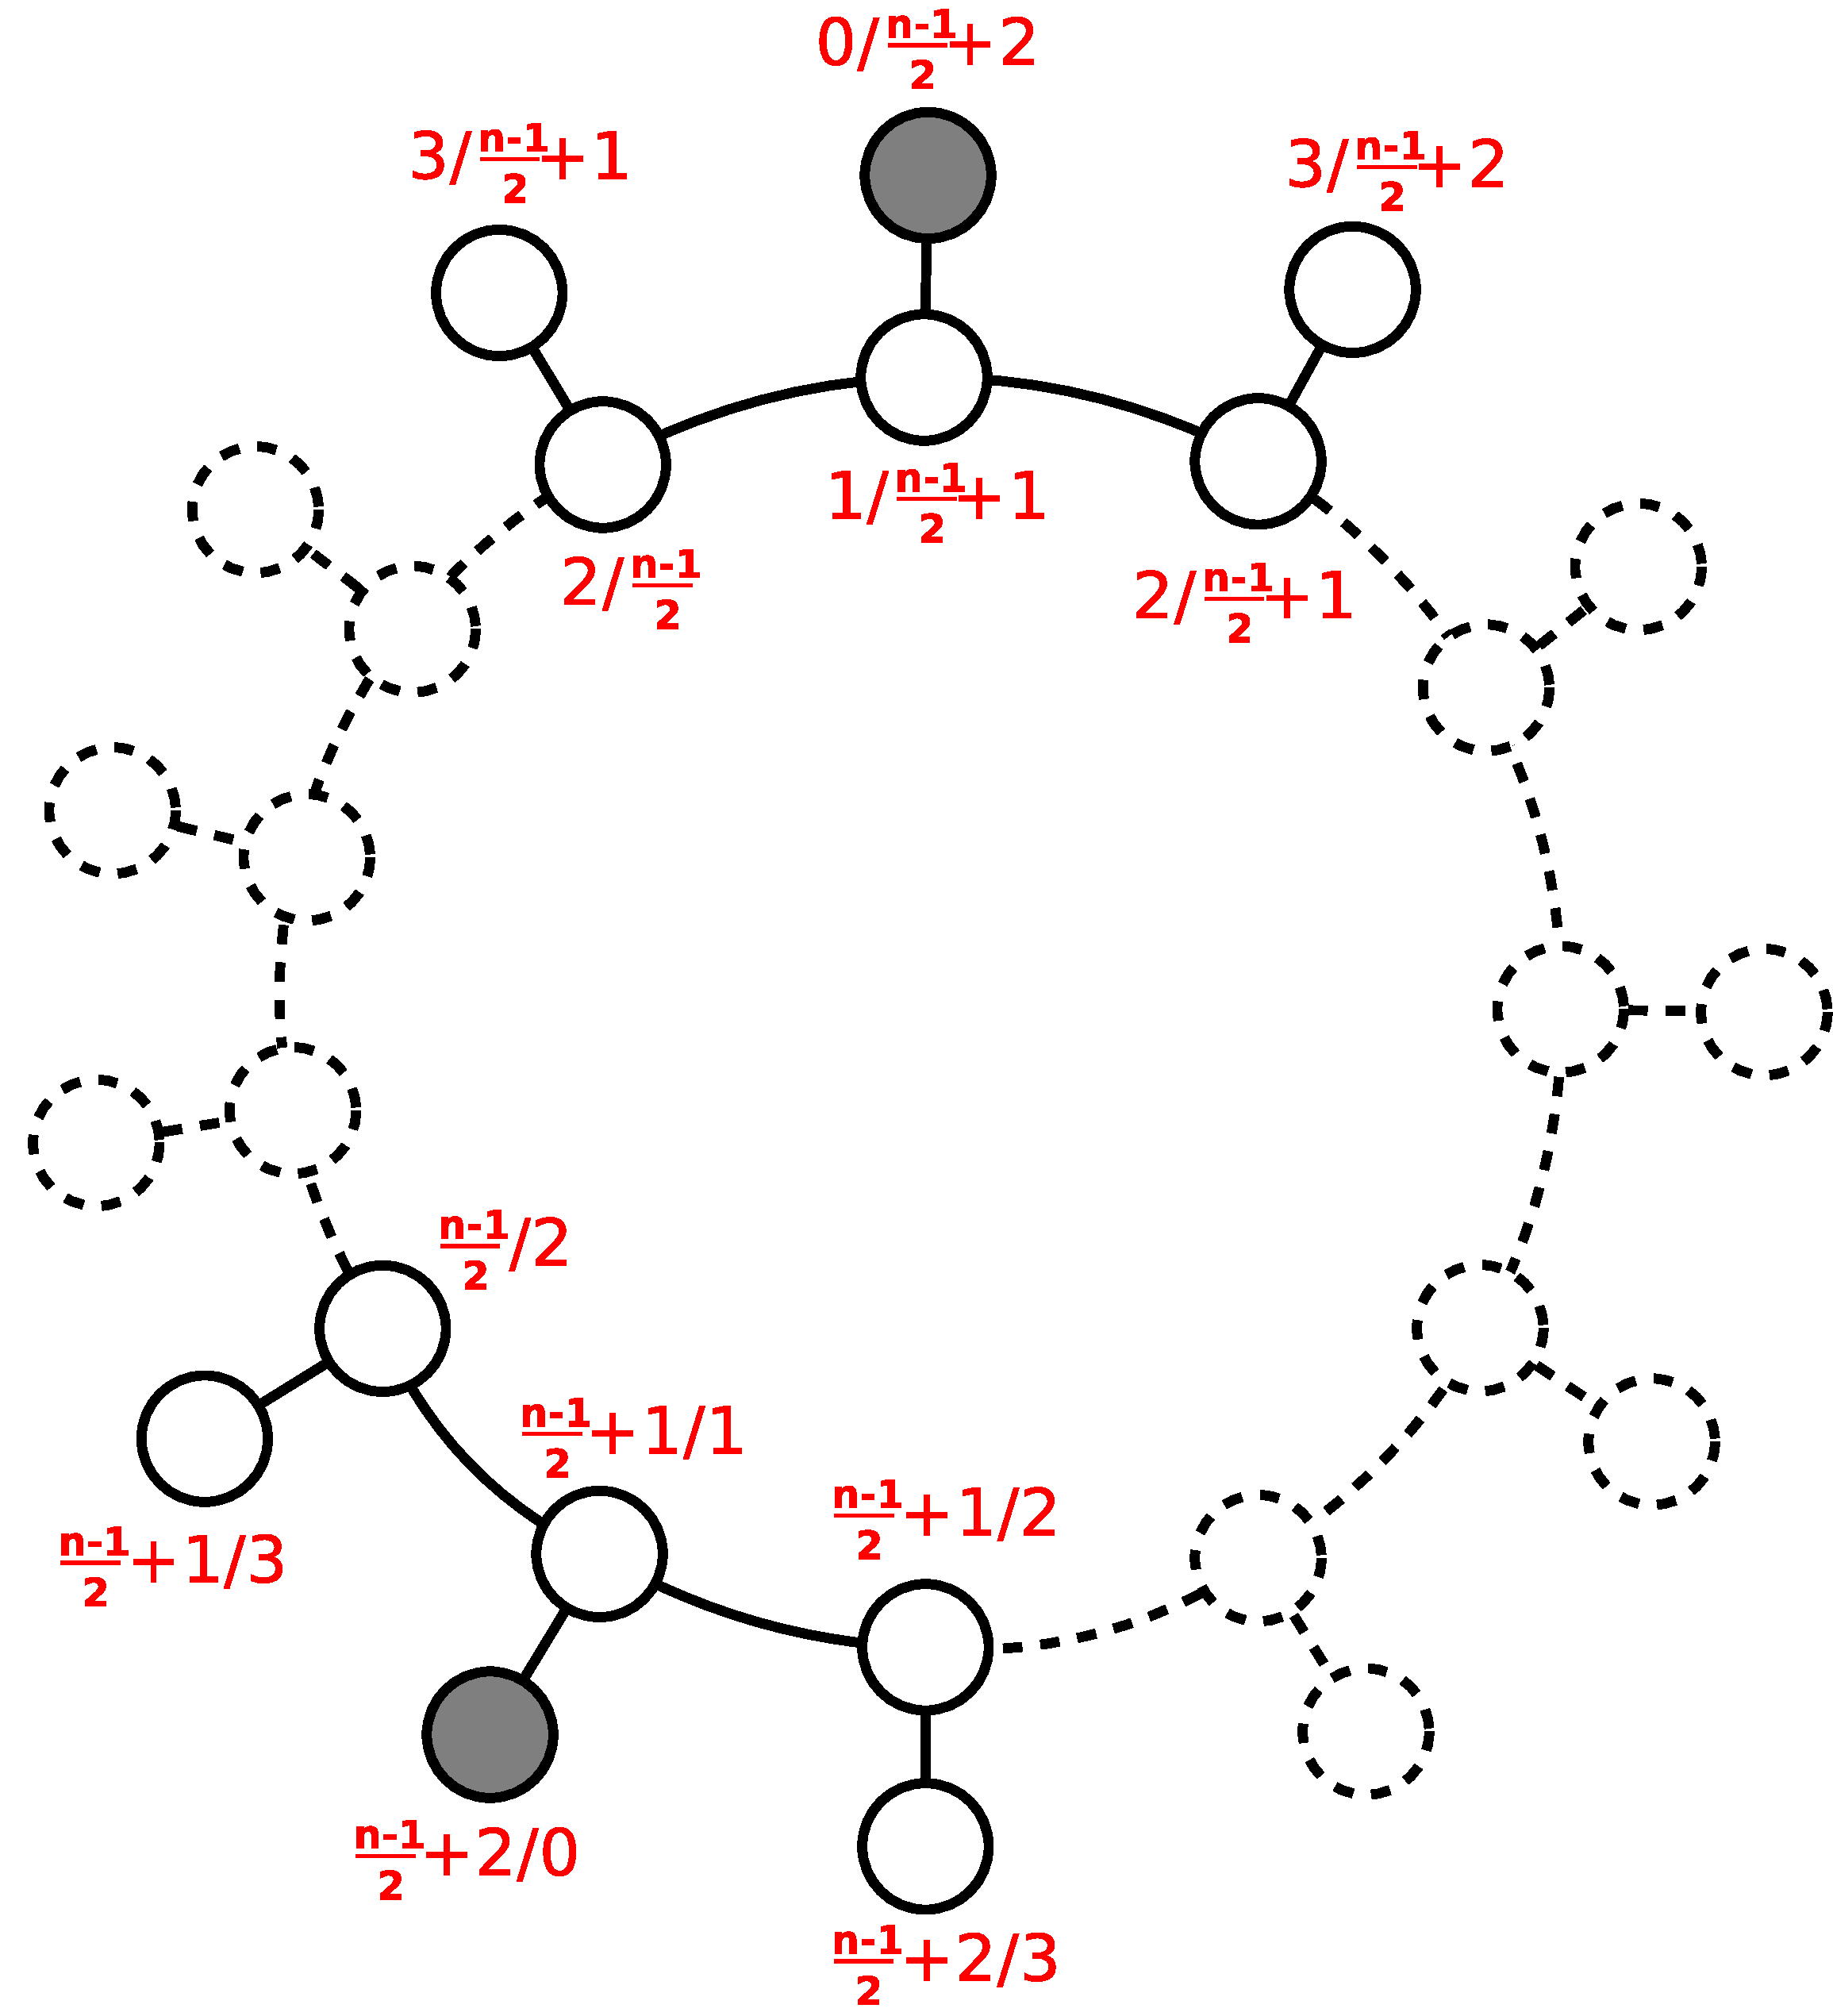
\includegraphics[width=170pt]{bilder/sonne2.pdf}
%  \caption{Der Sonnengraph $S_{2n,2}$}
%	\label{Bild2}
%\end{minipage}
%\end{figure}
%\vspace{-7mm}
\vspace{-8mm}
 \begin{figure}[h!]
		\centering
 		 \includegraphics[width=120pt]{bilder/gbsbspsonne2glr.pdf}
   \caption{Ein $C_{n}$-Blatt mit zwei Knoten in der metrischen Basis, welche die Bedingung von Lemma \ref{Bifurnachbar} erfüllen}
  	 \end{figure}
\vspace{-4mm}
  	 ~\linebreak

\begin{proof}[Beweis:]~
Für den ersten Knoten in der metrischen Basis gibt es $2n$ Möglichkeiten, aber nur $n$ unterschiedliche Fälle. Denn wird der erste Knoten aus einem Strahl aufgenommen, so gilt nach Lemma \ref{bifur}, dass der Strahlursprung als Element der metrischen Basis betrachtet werden kann.\\
Der zweite Knoten muss die Bedingung vom Lemma \ref{Bifurnachbar} erfüllen. Es bleiben noch genau drei mögliche Knoten $v_{\frac{n}{2}}$, $v_{\frac{n-1}{2}}$ und $v_{\frac{n+1}{2}}$ als zweiter Ankerknoten.\\ 
Der Knoten $v_{\frac{n}{2}}$ kann nicht aufgenommen werden, da zwei gegenüberliegende Knoten einen Kreis gerader Länge nicht trennen.\\
Durch die Wahl von $v_{\frac{n-1}{2}}$ oder $v_{\frac{n+1}{2}}$ entstehen mindestens zwei Markierungen der Form $a/b$ und $a+1/b+1$ auf dem Kreis. Da jeder Knoten ein Strahlursprung ist, gibt es in dem Graphen einen weiteren Knoten mit der Markierung $a+1/b+1$. Zur Veranschaulichung wird der Graph $S_{6,2}$ betrachtet.
\begin{figure}[h!]
		\centering
 		 \includegraphics[width=120pt]{bilder/bspsonne6.pdf}
   \caption{Ein markierter $S_{6,2}$ mit zwei Knoten in der MB}
  	 \end{figure}
\end{proof}
\begin{lem}
Ein ungerader Sonnengraphen $S_n$ mit $n\geq 3$ ist getrennt wenn der maximale Abstand zwischen zwei Strahlursprüngen mit einem Ankerknoten $max\;dist(r_i,r_j)\leq \frac{n+3}{2}$ mit $r_i,r_j \in R$ und $r_j\neq r_i$.
\end{lem}
\begin{comment}
\begin{proof}[Beweis:]
Angenommen zwei Knoten sind nicht getrennt. Bei einem ungeraden Sonnengraph sind zwei Knoten nur dann ungetrennt wenn sie einen gemeinsamen Bifurkator haben. Bei Strahlen der Länge eins
\end{proof}
\end{comment}
\begin{lem}
Ein gerader Sonnengraphen $S_n$ mit $n\geq 6$ ist getrennt wenn der maximale Abstand zwischen zwei Strahlursprüngen mit einem Ankerknoten $max\;dist(r_i,r_j)\leq \frac{n+4}{2}$ mit $r_i,r_j \in R$ und $r_j\neq r_i$.
\end{lem}
\begin{lem}
Ist in einem ungeraden Sonnengraphen $S_n$ mit $n\geq 3$ mindestens ein Ankerknoten oder sind in einem gerade Sonnengraphen $S_m$ mit $m\geq 6$ mindestens zwei Ankerknoten so reicht die Aufnahme von einem weiteren Knoten in die metrische Basis um den Graphen zu trennen. 
\end{lem}
\begin{proof}[Beweis:]
Der größte Abstand ohne Ankerknoten bei einem ungeraden Sonnengraphen mit mindestens einem Ankerknoten ist $n-1$. Setzt man den Knoten genau in die Mitte von diesem Weg, so schrupft die maximal Distanz zwischen Ankerknoten aus $\frac{n-1}{2}<\frac{n+5}{2}$.\newline\newline
Die maximale Distanz zwischen mindestens zwei Ankerknoten auf einem geraden Sonnengraphen ist $n-2$, dies ist der Fall wenn es genau zwei Ankerknoten gibt und diese nebeneinander liegen. Positioniert man den Knoten genau in die Mitte des Weges, so ist die neue maximale Distanz $\frac{n-2}{2}<\frac{n+4}{2}$.
\end{proof}

%\begin{proof}[Beweis:]
%\begin{figure}[h!]
%		\centering
% 		 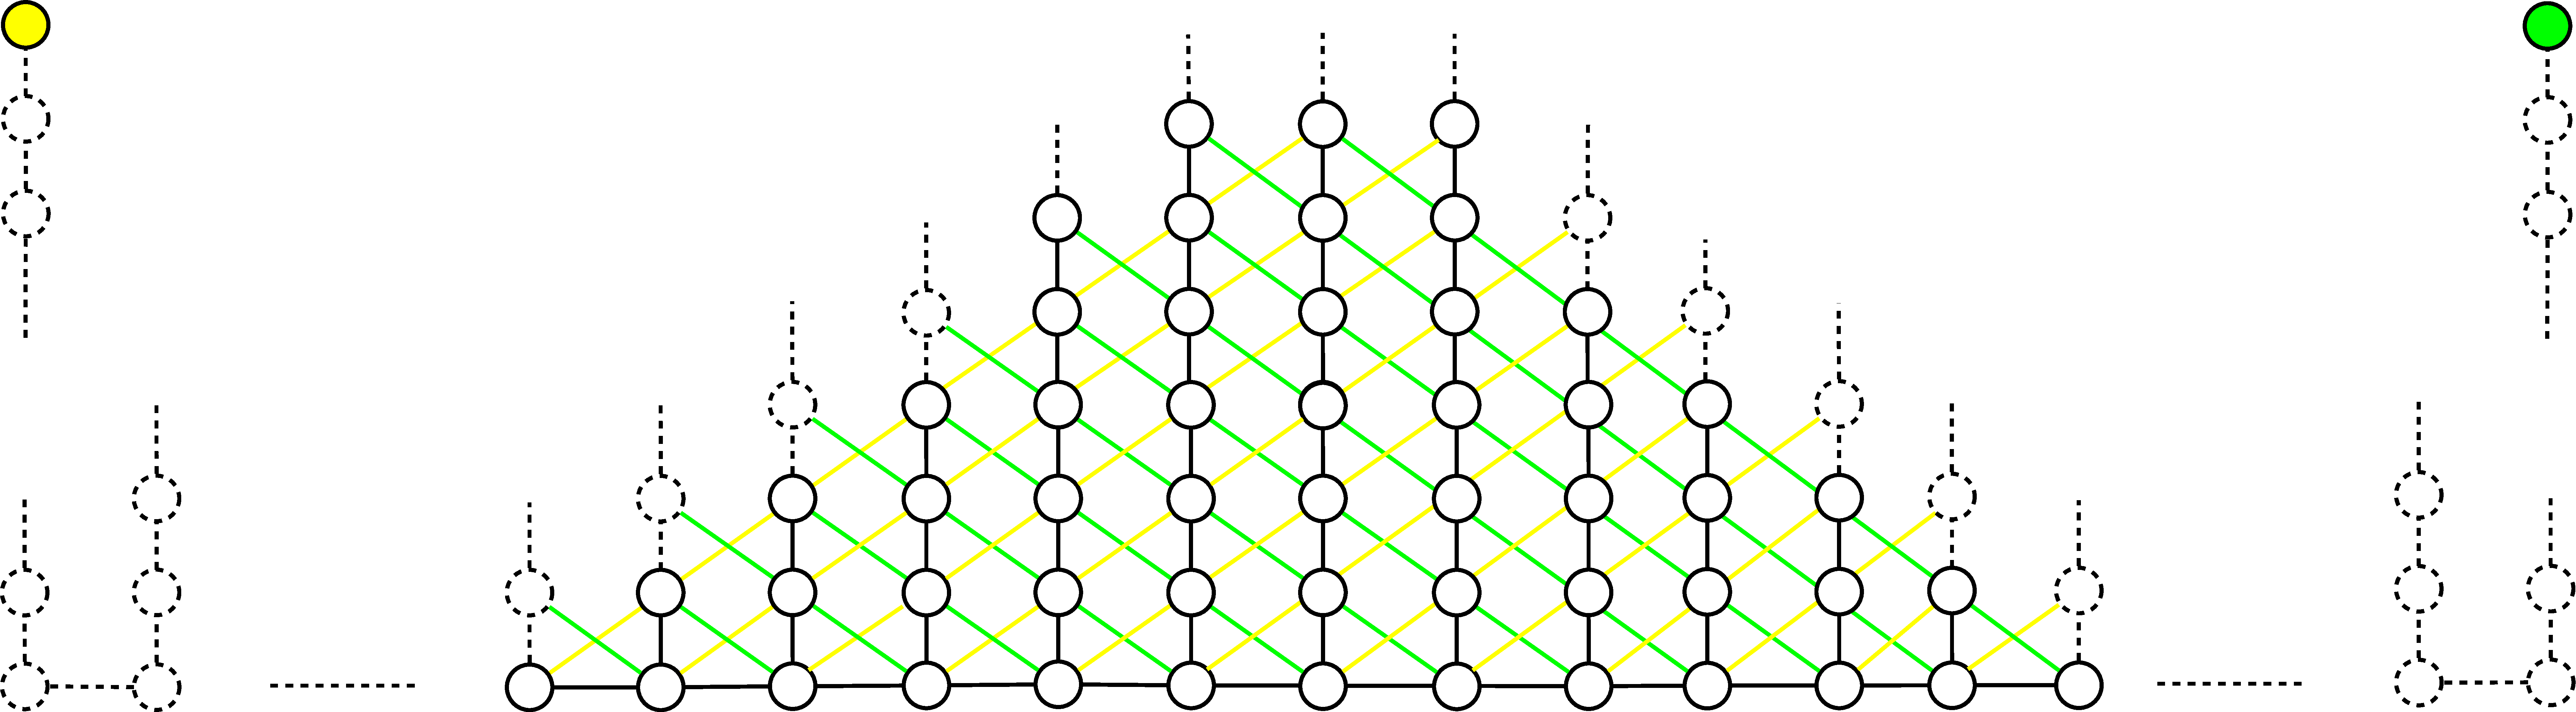
\includegraphics[width=430pt]{bilder/sonne1.pdf}
%   \caption{Ein $C_{n}-Blatt$ wird durch zwei Knoten getrennt}
%  	 \end{figure}
%Jeder Knoten auf einem Strahl hat eine $a+x/b+x$ Markierung mit $0 \leq x \leq k$ und $a/b$ die Markierung des Strahlursprung auf dem Kreis $C_n$.
%\end{proof}
\subsection{Metrische Dimension unvollständiger Sonnengraphen}  	
\label{chap_usonne} 
\begin{defi}{\textbf{(Unvollständiger Sonnengraph $S'_{n,k}$)}}\\
Sei ein Kreis $C_n$ für $n \geq 3$ mit der Knotenmenge $|V|=\{ c_1, \ldots , c_n \}$ und $n'$ Weggraphen $P_{k'}$ mit $1 \leq n' \leq n-1$ für $2 \leq k' \leq k$ gegeben. Die Knoten mit Grad eins auf dem $i-$ten Weg werden als $v_{i,1}$ und $v_{i,k-1}$ bezeichnet. Durch das Hinzufügen von $n'$ neuen Kanten der Form $\{v_{i,1},c_i\}$ für $1 \leq i \leq n$ ensteht der zusammenhängende Sonnengraph $S'_{n',k'}$. Gibt es mindestens zwei Strahlen mit unterschiedlicher Länge, so wird der unvollständige Sonnengraph als $S'_n$ bezeichnet. 
\end{defi}
\begin{bem}
Jeder unvollständige Sonnengraph ist ein Teilgraph eines Sonnengraphen und wird von dessen metrische Basis getrennt. Sind die Strahlen mit den Ankerknoten in dem unvollständigen Sonnengraphen nicht vorhanden, so können die Strahlurprungsknoten als Ankerknoten verwendet werden. Nach Lemma \ref{knotenimstrahl} trennen zwei Knoten in einem Strahl die gleichen Knotenpaare in dem Graphen ohne den Strahl selbst.
\end{bem}
\begin{lem}
\label{schrankenunvsg}
Für die metrische Dimension eines unvollständigen Sonnengraphen $S'_{n}$ gilt:
$$\beta(C_n) \leq \beta(S'_{n})\leq \beta(S_{n})$$
\end{lem}
\begin{proof}[Beweis:]
Um einen unvollständigen Sonnengraphen aus einem Kreis $C_n$ zu erhalten wird mindestens ein neuer Knoten erzeugt und mit genau einem Knoten in dem Graphen $C_n$ verbunden. Dieser Vorgang wird wiederholt bis der gewünschte unvollständige Graph erzeugt ist. Um einen Sonnengraphen $S_{n}$ aus einem unvollständigen Sonnengraphen zu erhalten wird mindestens ein Knoten hinzugefügt und mit genau einer Kante verbunden. Nach Lemma \ref{dist} gilt für die metrische Dimension:
$$\beta(C_n)  \leq \beta(S'_{n}) \leq \beta(C_n) +1 \text{ und } \beta(S'_{n}) \leq \beta(S_n) \leq \beta(S'_{n})+1$$
\end{proof}
\begin{bem}
Nach Lemma \ref{schrankenunvsg} gilt für $n=2k+1$ für $k \in \mathbb{N}$: $$2=\beta(C_n) \leq \beta(S'_{n,k})\leq \beta(S_{n,k})=2$$
Daraus folgt, dass die metrische Dimension eines unvollständigen Sonnengraphen $S'_{n,k}$ mit $n=2k+1$ für $k \in \mathbb{N}$ zwei ist.\\
Für die metrische Dimension für $n=2k+2$ für $k \in \mathbb{N}$ gilt: $$2=\beta(C_n) \leq \beta(S'_{n,k})\leq \beta(S_{n,k})=3$$
Daraus folgt, dass die metrische Dimension eines unvollständigen Sonnengraphen $S'_{n,k}$ mit $n=2k+2$ für $k \in \mathbb{N}$ entweder zwei oder drei ist. Um die metrische Dimension genau zu bestimmen werden $\frac{n}{2}$ unterschiedliche Fälle aus der Tabelle \ref{fallunterscheidungungeradesonnen2md} betrachtet.
\end{bem}
\begin{lem}
\label{usg}
Ist $max\;dist(r_i,r_j)\geq \lceil \frac{n+3}{2}\rceil$ kann der unvollständige Sonnengraph getrennt sein. Ist der Sonnergraph ungerade, so ist er durch zwei Ankerknoten getrennt oder durch drei Ankerknoten, wenn er gerade ist, wenn es keine Strahlen gibt auf allen Knoten $v$ mit der Eigenschaft,\\
$v$ liegt zwischen den Knoten $r_i$ und $r_{j+\lfloor\frac{n}{2}\rfloor}$ (gezählt auf der Seite wo $r_i$ liegt) \\und $v$ liegt zwischen den Knoten $r_j$ und $r_{i+\lfloor\frac{n}{2}\rfloor}$ (gezählt auf der Seite wo $r_j$ liegt)
\end{lem}
\begin{table}[htp]
\centering
 \renewcommand{\arraystretch}{2}
\begin{tabularx}{\textwidth}{||c|c||}
\hline\hline
\vspace{0.3mm}
1. Fall& \multirow{3}{121mm}{$\frac{n}{2}-2$ benachbarte Knoten ohne Strahlen}\\
\cline{1-1}
\vspace{-6mm}
&\\
	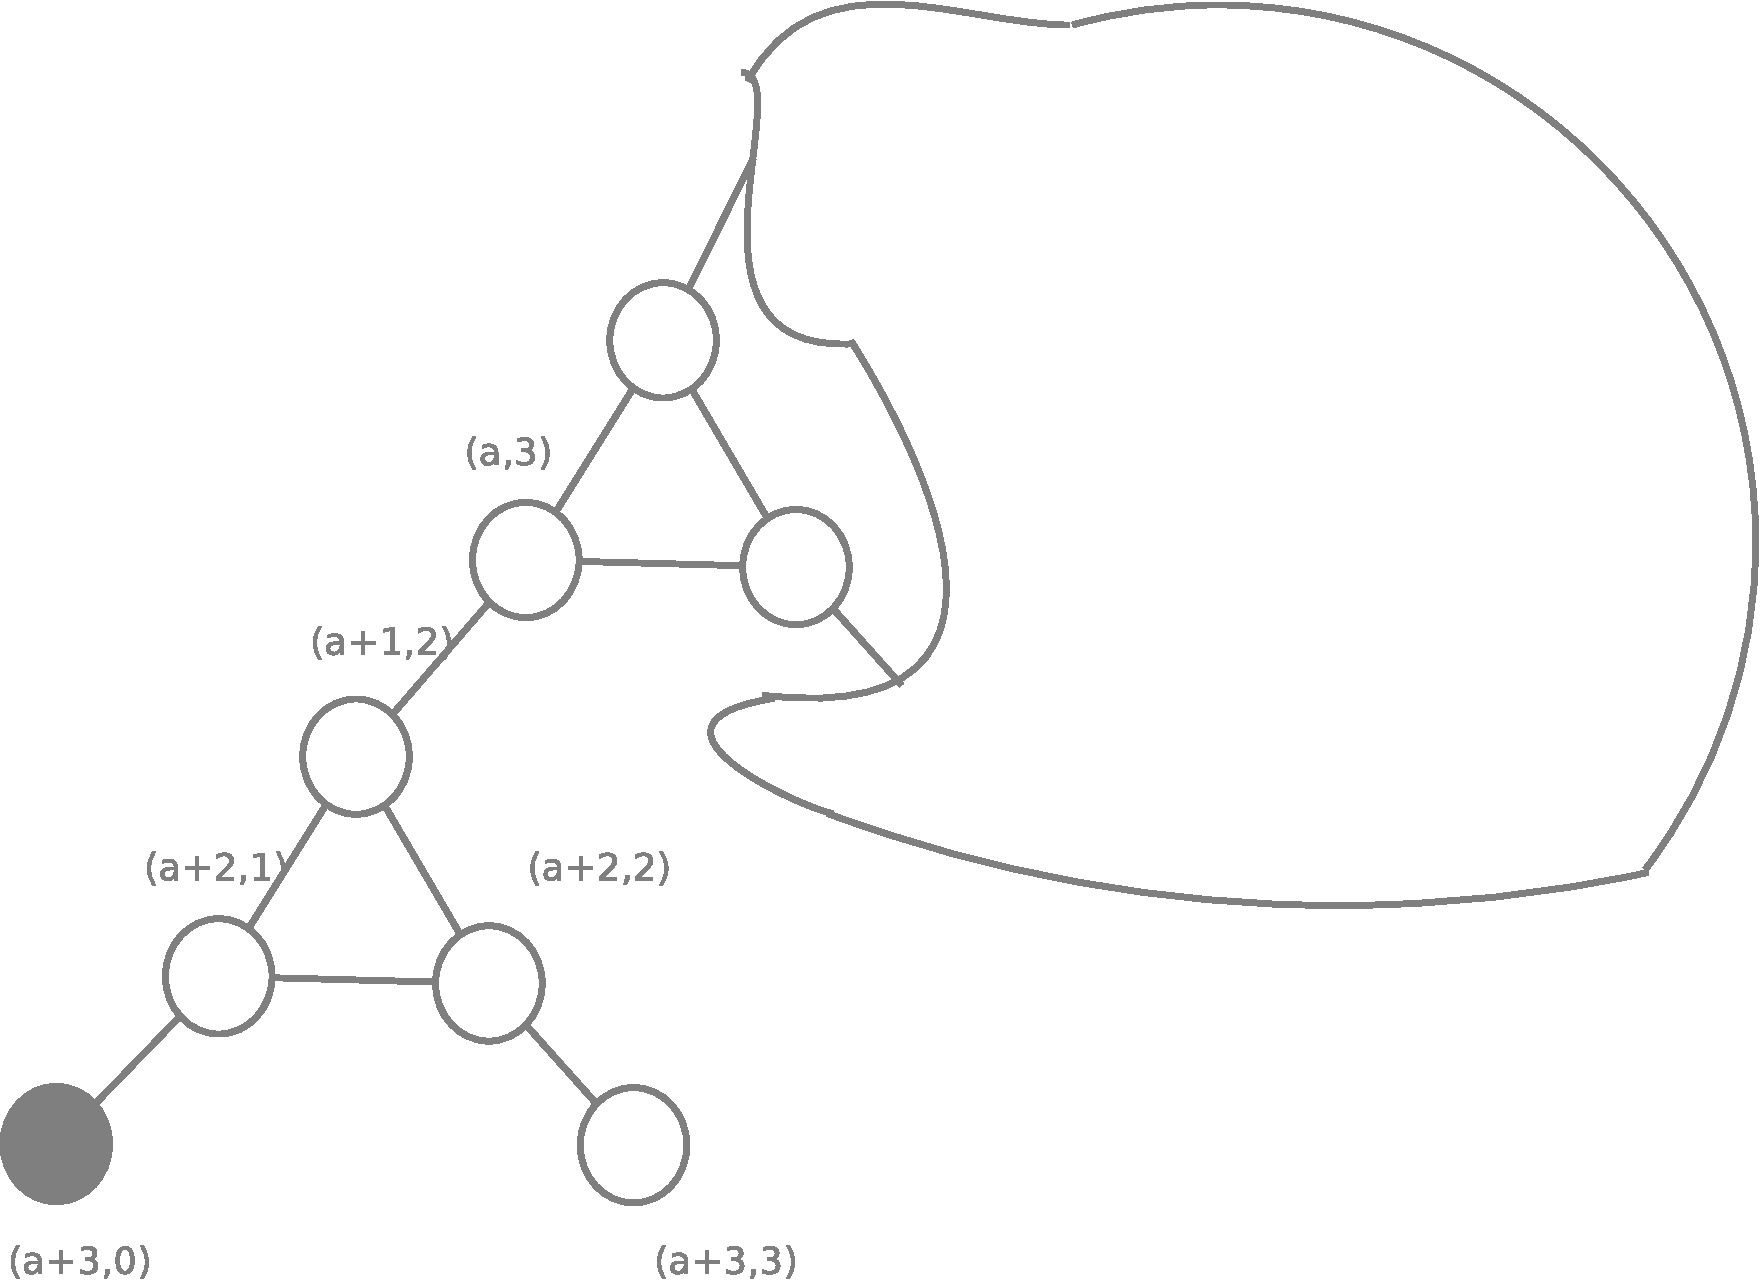
\includegraphics[width=50pt]{bilder/fall1.pdf}&\\
\hline\hline
\vspace{0.3mm}
2. Fall&\multirow{3}{121mm}{$2$ antipodale Knoten ohne Strahlen, $2$ Knoten mit/ohne Strahlen und $\frac{n}{2}-3$ Knoten ohne Strahlen der Länge $2$}\\
\cline{1-1}
\vspace{-6mm}&\\
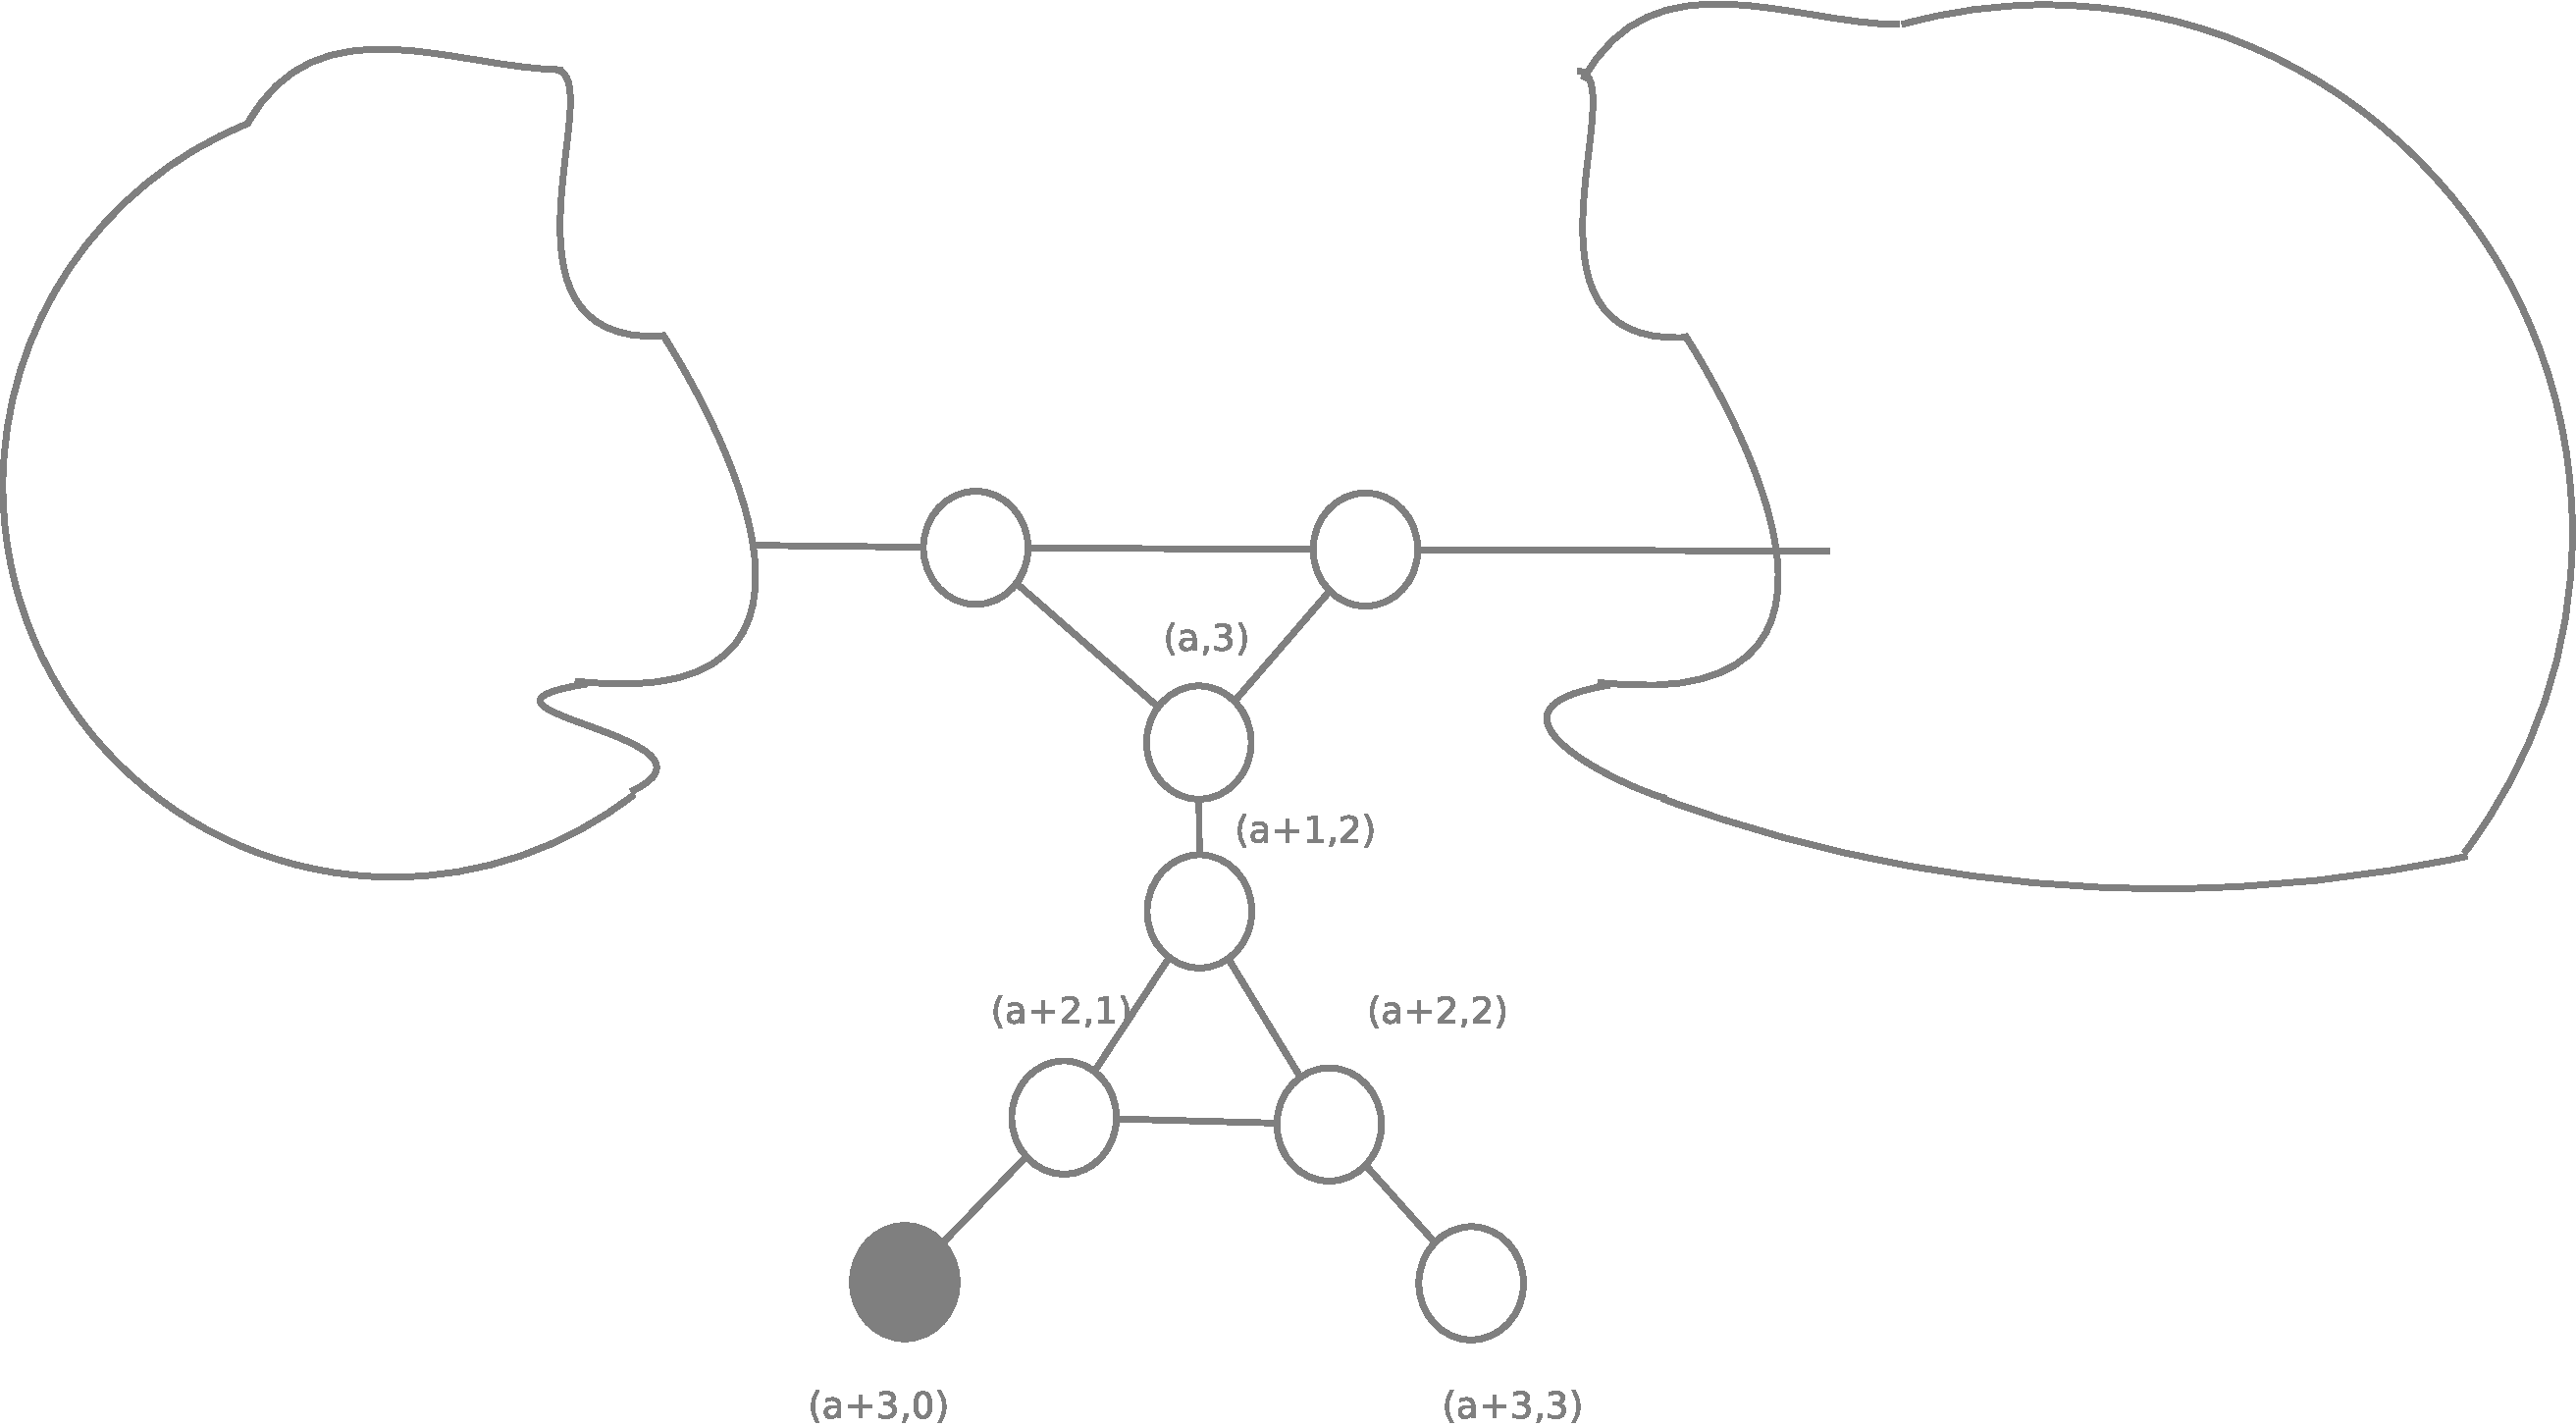
\includegraphics[width=50pt]{bilder/fall2.pdf}&\\
\hline\hline
\vspace{0.3mm}
3. Fall&\multirow{3}{121mm}{ $4$ antipodale Knoten ohne Strahlen (je $2$), $2$ Knoten mit/ohne Strahlen und $\frac{n}{2}-4$ Knoten ohne Strahlen der Länge $3$}\\
\cline{1-1}
\vspace{-6mm}&\\
\includegraphics[width=50pt]{bilder/fall3.pdf}&\\
\hline\hline
$\cdot$ &  $\cdot$\\
$\cdot$ &  $\cdot$\\
$\cdot$ &  $\cdot$\\
\hline\hline
\vspace{0.3mm}
$\frac{n}{2}-2$. Fall&\multirow{3}{121mm}{$n-2$ antipodale Knoten ohne Strahlen (je $\frac{n}{2}-1$), $2$ Knoten mit/ohne Strahlen und $1$ Knoten ohne Strahlen der Länge $\frac{n}{2}-1$}\\
\cline{1-1}
\vspace{-6mm}&\\
\includegraphics[width=50pt]{bilder/fall4.pdf}&\\
\hline\hline
\vspace{0.3mm}
$\frac{n}{2}-1$. Fall&\multirow{3}{121mm}{$n-4$ antipodale Knoten ohne Strahlen (je $\frac{n}{2}-2$)}\\
\cline{1-1}
\vspace{-6mm}&\\
\includegraphics[width=50pt]{bilder/falln2-1.pdf}&\\
\hline\hline
\end{tabularx}
\caption{Unvollständige Sonnen mit metrischer Dimension zwei}
\label{fallunterscheidungungeradesonnen2md}
\end{table}
%%%%%%%%%%%%%%%%%%%%%%%%%%%%%%%%%%%%%%%%%%%%%%%%%%%%%%%%%%%%%%%%%%%%%%%%%%%%%%%%%%%%%%%%%%%%%%%%%%%%%%%%%%%%%%%%%%%%%%%%%%%%%%%%
\newpage
\section{Metrische Dimension der Freundschaftsgraphen $F_{n}$}
\vspace{-3mm}
"Haben je zwei Bekannte einen weiteren gemeinsamen Bekannten und sie sind untereinander bekannt, so gibt es eine Person, welche alle anderen kennt". Diese Behauptung kann als ein Graphenproblem definiert werden, wobei Knoten Personen und Kanten Bekannschaften repräsentieren. Um es zu lösen wurde von Paul Erdős et al. \cite{Erdos} der Freundschaftsgraph eingeführt. In der Arbeit "The resolving graph of amalgamation of cycles" \cite{amal} wird die metrische Dimension von Freundschaftgraphen bestimmt. Der Schwerpunkt dieser Arbeit liegt auf der Anzahl der unterschiedlichen metrischen Basen.
\begin{defi}{\textbf{(Freundschaftsgraph $F_{n,3}$)}}\\
Der Freundschaftsgraph $F_{n,3}=(V,E)$ besteht aus der Knotenmenge $$V = \{u,v_{1,1},v_{1,2},v_{2,1},v_{2,2},\ldots,v_{n,1},v_{n,2}\}$$ und der Kantenmenge $$E = \{ \{u,v_{1,i}\}~|~ 1 \leq i \leq n \} \cup \{ \{u,v_{i,2}\}~|~ 1 \leq i \leq n \} \cup \{ \{ v_{i,1}, v_{i,2} \} ~|~ 1 \leq i \leq n \}$$
Die Kanten $\{u,v_{i,1}\},\;\{u,v_{i,2}\}$ und $\{v_{i,1},v_{i,2}\}$ bilden den $i$-ten Kreis $C_3$.
\end{defi}
\begin{bsp}~
\vspace{-4mm}
\begin{figure}[h!]
\centering
 		 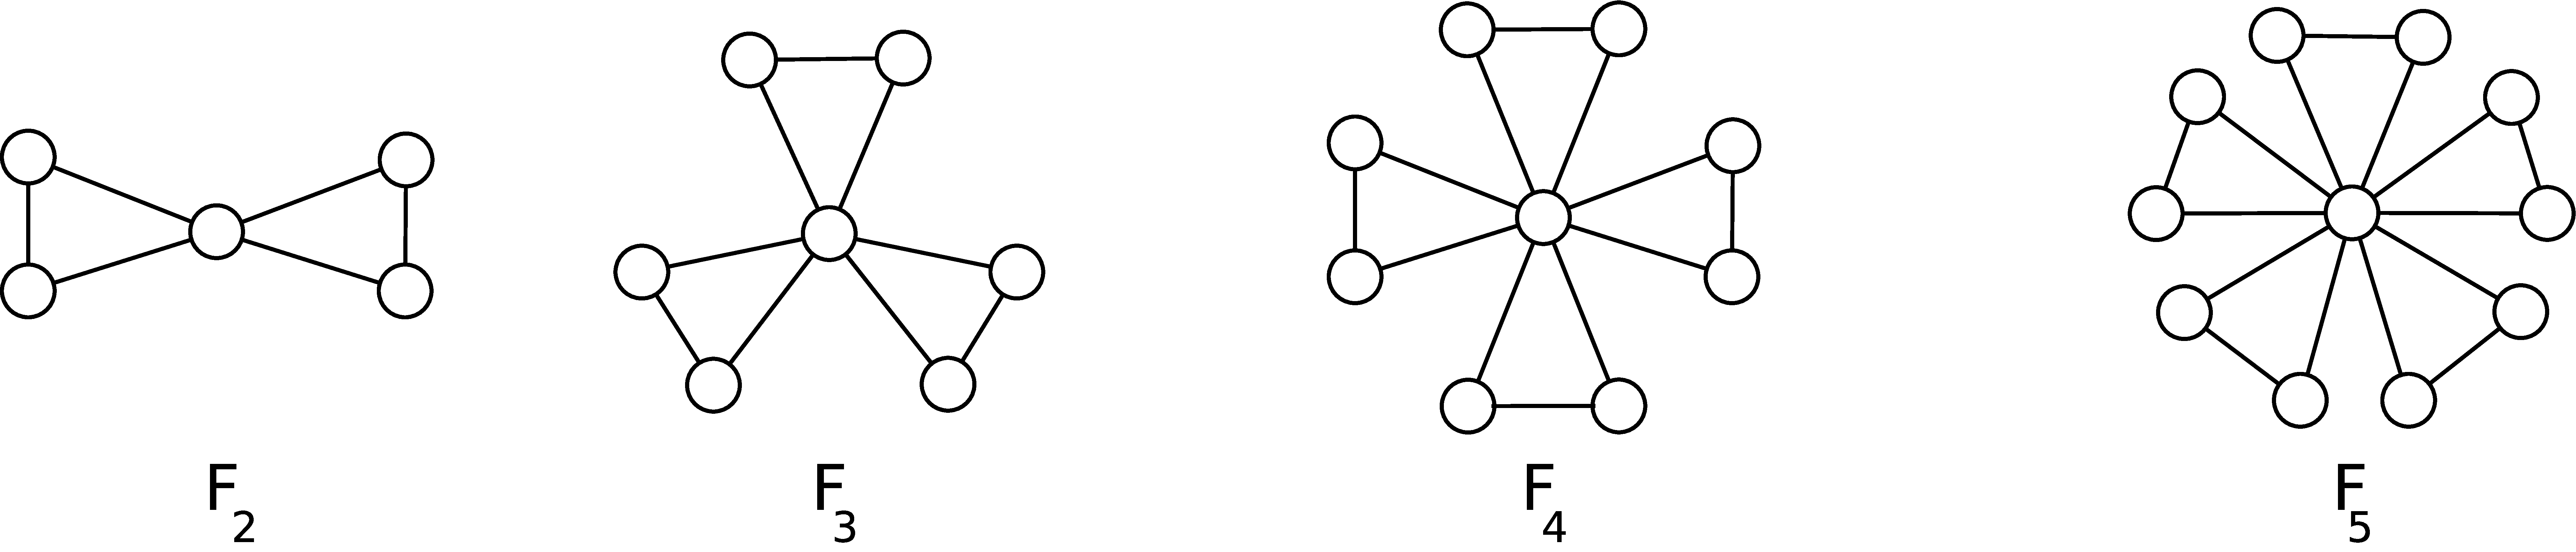
\includegraphics[width=360pt]{bilder/freunschaftsgraph.pdf}
   \caption{Vier Freundschaftsgraphen}
   \label{bild:fg}
\end{figure}
\vspace{-3mm}
\end{bsp}
\begin{lem}
\label{Freundschaftsgraphen}
Die metrische Dimension eines Freundschaftsgraphen $F_{n,3}$ ist $n$.
\end{lem}
\vspace{-2mm}
Um diese Behauptung zu beweisen, wird das folgende Lemma benötigt. 
\begin{lem}
\label{mindfreundschaftsgraph}
Sei ein Freundschaftsgraph $F_{n,3}$ gegeben. Jede metrische Basis muss aus dem $i$-ten $C_3$ mindestens einen der folgenden Knoten $\{v_{i,1},v_{i,2}\}$ beinhalten. 
\end{lem}
$Beweis:$
\vspace{-7mm}
\begin{figure}
\vspace{-7mm}
\begin{minipage}[l]{170pt}
\centering
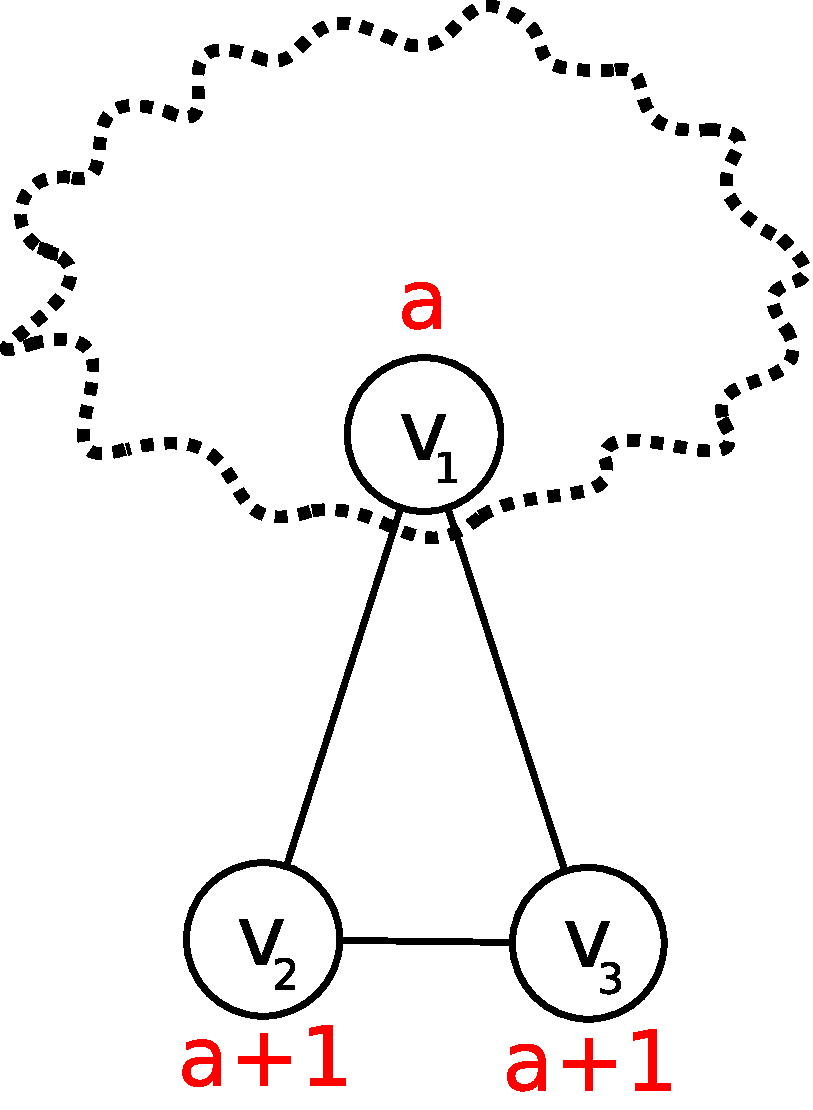
\includegraphics[width=90pt]{bilder/freundschaftsgraphbew.pdf}
\caption{Ein markierter $C_3$}
\end{minipage}
\begin{minipage}[r]{250pt}
Angenommen es gibt einen $C_3$ ohne Ankerknoten. Durch die eindeutige Verbindung zu dem Restgraphen, welche über einen Trennungsknoten läuft, folgt aus Symmetriegründen, dass die Knoten $v_{i,1}$ und $v_{i,2}$ identische Markierungen haben.\\Dies ist ein Widerspruch zu der Definition einer metrischen Basis.\\
Die metrische Dimension eines Freundschaftsgra-\\phen $F_{n,3}$ ist mindestens gleich der Anzahl seiner $C_{3}$,\\mindestens $n$.$\;\;\;\;\;\;\;\;\;\;\;\;\;\;\;\;\;\;\;\;\;\;\;\;\;\;\;\;\;\;\;\;\;\;\;\;\;\;\;\;\;\;\;\;\;\;\;\;\;\;\;\;\;\;\;\;\;\square$
\end{minipage}
\end{figure}

\newpage
\begin{proof}[Beweis von Lemma \ref{Freundschaftsgraphen}:] \vspace{+1mm} ~ \linebreak
Nach Lemma \ref{mindfreundschaftsgraph} ist bekannt, dass die metrische Dimension eines Freundschaftsgraphen $F_{n,3}$ mindestens $n$ ist. Angenommen, alle als $v_{2,i}$ markierten Knoten werden in die metrische Basis aufgenommen. Dann sind sie getrennt. Der Knoten $v_1$ hat die Distanz eins zu allen Knoten in der metrischen Basis und ist der einzige Knoten mit dieser Eigenschaft. Für jeden Knoten $v_{3,i}$ gibt es genau einen Knoten $v_{2,i}$ mit der Distanz eins. Zu allen anderen Knoten in der metrischen Basis hat jeder Knoten $v_{3,i}$ die Distanz zwei. Alle Markierungen sind eindeutig und der gesamte Graph ist durch die $n$ Knoten getrennt.
\end{proof}
\vspace{-14mm}
~ \linebreak
\begin{defi}{\textbf{(Freundschaftsgraph $F_n$)}}\\
%Der $k$-fache Freundschaftsgraph $F_{n,k}=(V,E)$ mit $k\geq 3$ besteht aus der Knotenmenge $$V = \{u,v_{1,1}, \ldots, v_{1,k-1},v_{2,1},\ldots v_{2,k-1},\ldots,v_{n,1},\ldots v_{n,k-1}\}$$ und der Kantenmenge $$E = \{ \{u,v_{1,i}\}~|~ 1 \leq i \leq n \} \cup \{ \{u,v_{i,k-1}\}~|~ 1 \leq i \leq n \}$$$$\cup \{ \{ v_{i,j}, v_{i,j+1} \} ~|~ 1 \leq i \leq n \text{ und }1 \leq j \leq k-2\}$$
Der Freundschaftsgraph $F_{n}=(V,E)$ mit $k_1,\ldots, k_n \geq 3 $ besteht aus der Knotenmenge $$V = \{u,v_{1,1}, \ldots, v_{1,k_1-1},v_{2,1},\ldots v_{2,k_2-1},\ldots,v_{n,1},\ldots v_{n,k_n-1}\}$$ und der Kantenmenge $$E = \{ \{u,v_{1,i}\}~|~ 1 \leq i \leq n \} \cup \{ \{u,v_{i,k_i-1}\}~|~ 1 \leq i \leq n \}$$$$\cup \{ \{ v_{i,j}, v_{i,j+1} \} ~|~ 1 \leq i \leq n \text{ und }1 \leq j \leq k_i-2\}$$
Die Kanten $\{u,v_{i,1}\},\;\{u,v_{i,k-1}\}$ und $\{v_{i,j},v_{i,j+1}\}$ für $1 \leq j \leq k_i-2$ bilden den $i$-ten Kreis $C_k$.
\end{defi}

\begin{lem} \cite{amal}
\label{verallgFreundschaftsgraphen}
Die metrische Dimension eines Freundschaftsgraphen $F_{n}$ mit $t_1$ Kreisen der Länge $k=2j+1$ für $j \geq 1$ und $t_2$ Kreisen der Länge $k=2j$ für $j \geq 2$ ist 
\begin{equation}
   \beta(F_{n,k})=
   \begin{cases}
     t_1 & \text{f\"ur } t_2=0 \\
     2\cdot t_2-1 & \text{f\"ur } t_1=0 \\
     t_1+ 2\cdot t_2-1 & sonst
   \end{cases}
\end{equation}
\end{lem}
\begin{lem}
Beinhaltet ein Freundschaftgraph mindestens zwei gerade $k_i$ und ist $n\geq 2$, so beinhaltet jede metrische Basis mindestens zwei Knoten aus jedem $i$-ten Kreis mit einem geraden $k_i$, außer in Einem.  
\end{lem}
\subsection{Metrische Dimension von allgemeinen Freundschaftgraphen und Bäumen}
\label{amal}
\begin{lem}
Sei ein Freundschaftgraph $F_n$ gegeben mit metrischer Dimension $m$ und ein Baum $T$, welcher kein Weg ist, gegeben mit metrischer Dimension $k$. Verbindet man den mittleren Knoten $u$ mit einem Knoten $v \in T$ und $deg(v)\geq 2$ so ist die metrische Dimension des neuen Graphen $m+k$.
\end{lem}

\begin{lem}
Sei ein Freundschaftgraph $F_n$ gegeben mit metrischer Dimension $m$, sei der mittleren Knoten $u$ die Wurzel von einem Baum $T$ mit metrischer Dimension $k$ und einem einfachen Weg $P$ oder der Endknoten von einem einfachen Weg $P$ und so ist die metrische Dimension des neuen Graphen $m+k+1$.
\end{lem}
%%%%%%%%%%%%%%%%%%%%%%%%%%%%%%%%%%%%%%%%%%%%%%%%%%%%%%%%%%%%%%%%%%%%%%%%%%%%%%%%%%%%%%%%%%%%%%%%%%%%%%%%%%%%%%%%%%%%%%%%%%%%%%%%
\newpage
\vspace{-2mm}
\chapter{Metrische Dimension von Kaktusgraphen}
\label{kapkaktus}
\begin{defi}
Als Kaktusgraph wird ein Graph bezeichnet, wenn alle seine Kreise paarweise kantendisjunkt sind, sich also höchstens einen gemeinsamen Knoten teilen.
\end{defi}
Jeder Graph mit höchstens einem Kreis gehört zu der Graphklasse der Kaktusgraphen.\newline Einige Beispiele von Kaktusgraphen sind Wege, Bäume, Kreise, Sterne, Sonnengraphen und die $C_j$-Bäume aus Kapitel \ref{kapcjbaume}.\newline Die Kaktusgraphen sind außenplanar \cite{graphclasses}. Für die außenplanaren Graphen existiert ein Polynomialzeit-Algorithmus zur Berechnung der metrischen Dimension aus "On the Complexity of Metric Dimension" \cite{aussenplanar}. Durch die spezifische Struktur von Kaktuspraphen lässt sich die metrische Dimension sogar in Linearzeit berechnen. Dieser Abschnitt präsentiert denn Algorithmus, die Analyse seiner Laufzeit und seine Korrektheit.
\begin{figure}[h!]
		\centering
 		 \includegraphics[width=420pt]{bilder/kaktusallg.pdf}
   \caption{Ein Kaktusgraph $G$}
   \label{gk}
  	 \end{figure}
  	 \vspace{-2mm}
\begin{algorithm}
\caption{Aufbau des Algorithmus zur Berechnung der MD von Kaktusgraphen}
\begin{algorithmic}
\vspace{2mm}
\REQUIRE{Ein ungerichteter Kaktusgraph $G$}
\vspace{2mm}
\ENSURE{Die metrische Dimension $\beta(G) \in \mathbb{N^+}$}
\vspace{2mm}
\STATE 1. Bestimmung zweifacher Zusammenhangskomponenten (ZZK) mit mindestens drei\\$\;\;\;\;$Kanten und Einordnung jedes Knotens zu einer der drei Klassen $\{0,i,A\}$ mit $i \geq 1$\\
\vspace{2mm}
\STATE 2. Erkennen von Amalgamationsknoten\\
\vspace{2mm}
\STATE 3. Berechnung der metrischen Dimension der zweifachen Zusammenhangskomponenten,\\$\;\;\;\;$Ersetzung dieser durch Bäume und Überprüfung der Amalgamationsknoten\\
\vspace{2mm}
\STATE 4. Berechnung der zusätzlichen metrischen Dimension von Amalgamationsknoten\\
\vspace{2mm}
\STATE 5. Berechnung der metrischen Dimension des Baumes
\vspace{2mm}
\end{algorithmic}
\end{algorithm}
\newpage
\section{Vorbereitung}
\vspace{-4mm}
In diesem Abschnitt werden Definitionen, welche in diesem Kapitel zur Berechnung der metrischen Dimension eines Kaktusgraphen verwendet werden, zusammengefasst.
\vspace{-2mm}\newline\newline
Gibt es im Graphen ZZK, so wird jede Kante $e$ aus einer ZZK mit $ZZK[e]=1$ markiert. Ist ein Knoten $v$ mit einer Kante $e$ inzident die mit $ZZK[e]=1$ markiert ist, so ist es auch der Knoten $v$ mit $ZZK[v]=1$, und sonst mit $ZZK[v]=0$.\vspace{-2mm}\newline\newline
Laut Definition sind in einem Kaktusgraphen alle ZZK Kreise, wobei eine Kante in maximal einem Kreis vorkommen darf. Die Endknoten dieser Kanten werden in drei Klassen unterteilt.
\begin{defi}[Klasse von einem Knoten]~\newline
Ein Knoten welcher in mindestens einer ZZK ist, bekommt eine Klasse:
\begin{itemize}
\item[\textbf{0}] Dieser Knoten hat nur Nachbarn aus der gleichen ZZK.
\item[\textbf{i}] Dieser Knoten hat drei Nachbarn, ein Nachbar liegt an einem einfachen Weg der Länge $i$ mit $i \geq 1$.
\item[\textbf{A}] Dieser Knoten hat mindestens drei Nachbarn und er gehört nicht zur Klasse $i$. Diese Knoten werden auch als $A$-Knoten bezeichnet.
\end{itemize}
\end{defi}\vspace{-1mm}
Ist an einem Knoten $v$ der Klasse $A$ ein induzierter einfacher Weg, so bekommt er die Markierung $Weg[v]=1$.

\begin{defi}[Komponente]~\newline
Als \textbf{Komponente} in einem Kaktusgraphen werden bezeichnet:\vspace{-1mm}
\begin{itemize}
\item ZZK mit ggf. induzierten einfachen Wegen an Knoten der Klasse $i$\vspace{-1mm}
\item maximale Teilgraphen inkl. Trennungsknoten welche Bäume, aber keine Wege sind 
\end{itemize}
\end{defi}
\vspace{-1mm}
\begin{defi}[Typ von einer ZZK]~\newline
Eine ZZK beinhaltet immer einen Kreis und kann an den Knoten einfache Wege haben. Die folgenden Aussagen gelten ohne Beachtung der $A$-Knoten.\vspace{-1mm} 
\begin{itemize}
\item[\textbf{K}] Jeder Knoten hat nur Nachbarn aus der gleichen ZZK. (Nur Typ $0$)\vspace{-1mm}
\item[\textbf{S}] Jeder Knoten hat drei Nachbarn, ein Nachbar liegt an einem induzierten einfachen Weg. (Nur Typ $i$)\vspace{-1mm}
\item[\textbf{US}] Es gibt jeweils mindestens einen Knoten von Typ $0$ und von Typ $i$.
\end{itemize}
\end{defi}
\vspace{-1mm}
\begin{defi}[Amalgamationsknoten]~\newline
Ein \textbf{Amalgamationsknoten} ist ein Knoten $v$ mit $deg(v)\geq 4$ und \vspace{-1mm}
\begin{itemize}
\item $ZZK[v]=1$ und $Weg[v]=1$\vspace{-1mm}
\item oder $v$ liegt in mindestens zwei unterschiedlichen ZZK.
\end{itemize}
\end{defi}
\vspace{-1mm}
\begin{defi}[Maximales Matching]~\newline
\vspace{-7mm}
\MP{{Maximales Matching}}
{Ein ungerichteter Baum $G=(V,E)$.}
{Ein maximales Matching $k$ die maximale Anzahl $k$ an Kanten,\\&so dass an jedem Knoten maximal eine Kante gewählt wurde.}
\end{defi}
\vspace{-5mm}
%Das Maximal Matching ist ein bekanntes NP-vollständiges Problem, welches für Bäume in Linearzeit gelöst wird.
\newpage
\section{Der Algorithmus zur Berechnung der metrischen Dimension von Kakturgraphen}
\textbf{Idee:} Ein Kaktusgraph wird in einen Baum mit gleicher metrischer Dimension umgewandelt, welche dann mit einem bekannten Linearzeit-Algorithmus bestimmt wird.\newline\newline
Zunächst wird der gegebene Kaktusgraph in unterschiedliche Komponenten aufgeteilt, welche durch genau einen Knoten verbunden sind. Diese Komponenten sind Kreise, Sonnen, unvollständige Sonnen und Bäume.\newline\newline
\begin{comment}
Wege werden nichts explizit als Komponenten aufgefasst, betrachte dazu die Arten von Wegen in einem Kaktusgraphen:
\begin{itemize}
\item Wege zwischen zweifachen Zusammenhangskomponenten
\item Wege an zweifachen Zusammenhangskomponenten
\begin{itemize}
\item an einem Knoten ist nur ein Weg
\item an einem Knoten ein Weg und noch etwas Anderes (kein Baum)
\end{itemize}
\end{itemize}
\end{comment}
Die Wege zwischen ZZK dürfen nach Lemma \ref{first_theorem} ignoriert werden. Die induzierten Wege an ZZK bilden mit der ZZK die Sonnen und unvollständigen Sonnen. Der letzte Fall von Wegen wird gesondert in dem Abschnitt zu Amalgamationsknoten untersucht.\newline\newline
Die ZZK sind Kreise, Sonnen und unvollständige Sonnen. Diese werden in Schritt 4 einzeln betrachtet, dabei werden Knoten welche diese Komponenten mit anderen Teilgraphen verbinden als $A$-Knoten markiert, sofern sich in dem Teilgraphen ein Ankerknoten befindet. Die metrische Dimension wird für jeden Kreis, jede Sonne und jede unvollständige Sonne bestimmt, mit der Voraussetzung, dass jeder $A$-Knoten ein Ankerknoten ist.\newline
Können die $A$-Knoten nicht alle Knotenpaare in einer Komponente trennen, so werden weitere Ankerknoten benötigt. Die Anzahl der zusätzlichen Ankerknoten bestimmt den Baum mit welchem die Komponente ersetzt wird. \newline\newline
Dadurch gibt es eine Trennung der Knoten innerhalb der Komponenten. Um die Trennung im gesamten Graphen zu erreichen, wird für jeden Knoten, welcher gleichzeitig in mehreren Komponenten ist, überprüft, ob seine Nachbarschaft getrennt ist. Die Anzahl der zusätzlich benötigten Ankerknoten um jede solche Nachbarschaft zu trennen wird in Schritt 5 ermittelt und bestimmt die letzte Veränderung des Baumes. Damit ist die Transformation abgeschlossen und die metrische Dimension des enstandenen Baumes kann mit der Formel aus Lemma \ref{baum} bestimmt werden.
\begin{bsp} An dem Kaktusgraphen $G_k$ aus der Abbildung \ref{gk} wird die Funktionsweise des Algorithmus gezeigt.\newline
\vspace{-3mm}
 	   	 \begin{figure}[h!]
		\centering
 		 \includegraphics[width=320pt]{bilder/kaktusallgschritt2.pdf}
   \caption{Die zweifachen Zusammenhangskomponenten wurden bestimmt und die Knoten wurden in drei Klassen partitioniert}
      \label{kaktus1}
  	 \end{figure} 
\newpage
In Abbildung \ref{kaktus1} wurde der Algorithmus \ref{alginit} ausgeführt und die zweifachen Zusammenhangskomponenten $\{1, \ldots, 7\}$ des Kaktusgraphen $G_k$ wurden in einer Liste von Listen gespeichert. Jeder Knoten wurde einer der Klassen $\{0,i,A\}$ mit $i \geq 1$ zugewiesen. Übersichtshalber wurde die Markierung $0$ in der Abbildung \ref{kaktus1} ausgelassen.
\vspace{-3mm} 	   	 
 	   	 \begin{figure}[h!]
		\centering
 		 \includegraphics[width=300pt]{bilder/kaktusallgschritt3,2.pdf}
   \caption{Die ZZK wurden in drei Klassen partitioniert}
      \label{kaktus1.2}
  	 \end{figure}
\vspace{-3mm}
  	 ~\linebreak
In Abbildung \ref{kaktus1.2} wurde der Algorithmus \ref{algeinteilung} bereits ausgeführt. Jede zweifache Zusammenhangskomponente wurde einzeln betrachtet und eindeutig als einer der drei Typen erkannt.\\
\vspace{-6mm}
  	   	\begin{figure}[h!]
		\centering
 		 \includegraphics[width=360pt]{bilder/kaktusallgschritt8.pdf}
   \caption{Amalgamationsknoten sind markiert und die MD von ZZK ist ausgerechnet}
\label{kaktus2}  	
  	 \end{figure}
  	 \vspace{-3mm}
~\linebreak
In der Abbildung \ref{kaktus2} wurden an den Knoten der Klasse $A$ mit dem Algorithmus \ref{alginit} bestimmt, ob es einen einfachen Weg an einem $A$-Knoten gibt. Mit dem Algorithmus \ref{algeinteilung} wurde die zusätzliche metrische Dimension der zweifachen Zusammenhangskomponenten berechnet. Außerdem wurden mittels Algorithmus \ref{algsonderfall1} die Amalgamationsknoten markiert.
\vspace{-3mm}
  	   	 \begin{figure}[h!]
		\centering
 		 \includegraphics[width=325pt]{bilder/kaktusallgschritt10.pdf}
   \caption{ZZK wurden ersetzt und die ungetrennten Amalgamationsknoten markiert}
   \label{kaktus4}
  	 \end{figure}
\newpage In Abbildung \ref{kaktus4} wurden alle ZZK durch Bäume ersetzt mit dem Algorithmus \ref{algreplace}. Weiterhin wurden die Amalgamationsknoten überprüft, so dass nur noch Amalgamationsknoten mit mindestens zwei ungetrennten Nachbarn in der Menge sind.\newline
\vspace{-1mm}
  	   	 \begin{figure}[h!]
		\centering
 		 \includegraphics[width=190pt]{bilder/matching.pdf}
   \caption{Der Baum $T$ wurde erzeugt und ein maximales Matching $M$ wurde bestimmt}
   \label{matching}
  	 \end{figure}
  	 \vspace{-3mm}
  	 ~\linebreak 
Der Algorithmus \ref{algsonderfall2} bestimmt die minimale Anzahl an Knoten, welche noch aufgenommen werden müssen. Dafür wird ein neuer Graph $T$ erschaffen und ein maximales Matching für diesen Graphen bestimmt. In diesem Beispiel gibt es zwei Amalgamationsknoten mit jeweils zwei ungetrennten Komponenten. Der Baum $T$ ist in Abbildung \ref{matching} dargestellt. Es gibt drei Kanten und das maximale Matching besteht aus zweien. Ein zusätzliches Element muss also in die metrischen Basis aufgenommen werden um beide Nachbarschaften der Amalgamationsknoten zu trennen.
\vspace{-1mm}
  	   	 \begin{figure}[h!]
		\centering
 		 \includegraphics[width=330pt]{bilder/kaktusallgschritt12.pdf}
   \caption{Resultierender Baum mit markierter metrischer Basis}
   \label{kaktus6}
  	 \end{figure}
  	 \vspace{-3mm}
  	 ~\linebreak 
  	 In Abbildung \ref{kaktus6} wird ein Knoten an den zuletzt betrachteten Amalgamationsknoten hinzugefügt, da es einen einfachen Weg an dem Knoten gibt. In so einem Fall reicht ein zusätzlicher Knoten aus um die metrische Dimension des Graphen um eins zu erhöhen.
  	
  	 \begin{figure}[h!]
		\centering
 		 \includegraphics[width=310pt]{bilder/kaktusallgschritt13.pdf}
   \caption{Der ursprüngliche Kaktusgraph mit markierter metrischer Basis}
   \label{kaktus7}
  	 \end{figure}
  	 \end{bsp}
  	 In Abbildung \ref{kaktus7} wird zum Vergleich eine metrische Basis des ursprünglichen Kaktusgraphen dargestellt. Ohne den Knoten $r_9$ wären die zwei hell- und dunkelroten Knotenpaare nicht getrennt.
  	 \clearpage
\section{Die Laufzeitanalyse}
~\linebreak
Um zu zeigen, dass die metrische Dimension von Kaktusgraphen in Linearzeit bestimmt werden kann wurde ein Algorithmus in Pseudocode geschrieben. In diesem Abschnitt wird seine Laufzeit analysiert. Es wird eine Übersicht über die einzelnen Algorithmen, eine kurze Beschreibung und eine obere Schranke für ihre Laufzeit in Tabelle \ref{übersicht1} angegeben.\newline
\vspace{-1mm}
\begin{table}[htp]
\centering
 \renewcommand{\arraystretch}{2}
\begin{tabularx}{\textwidth}{@{\extracolsep{\fill}}|c|c|c|}
\hline
\textbf{Algorithmus}&\textbf{Bedeutung}&\textbf{Laufzeit}\\
\hline
\vspace{-1mm}
\multirow{3}{26mm}{Algorithmus \ref{alginit}}& Bestimmung ZZK und Einteilung der &\multirow{3}{*}{$\mathcal{O}(|V|+|E|)$}\\
\vspace{-1mm}
&Knoten in den ZZK in Klassen und Überprüfung&\\&an welchen $A$-Knoten es einen einfachen Weg gibt&\\
\hline
\vspace{-1mm}
\multirow{2}{25mm}{Algorithmus \ref{algeinteilung}}&Partitionierung der ZZK in drei Typen&  \multirow{2}{22mm}{$\mathcal{O}(|V|+|E|)$}\\&$K$, $S$ und $US$ und Aufruf zur Berechnung der MD&\\
\hline
Algorithmus \ref{algsonderfall1}& Amalgamationsknoten werden markiert & $\mathcal{O}(|V|+|E|)$\\
\hline
Algorithmus \ref{algberechnungkreis}& Die zusätzliche MD von Kreisen wird bestimmt & $\mathcal{O}(|1|)$\\
\hline
Algorithmus \ref{algberechnungsonne}& Die zusätzliche MD von Sonnen wird bestimmt & $\mathcal{O}(|1|)$\\
\hline
\multirow{2}{26mm}{Algorithmen \ref{algberechnungungeradesonne1}, \ref{algberechnungusonne2}, \ref{algberechnunggeradesonne1} und \ref{algberechnungungeradesonne0}}& Die zusätzliche MD von & \multirow{2}{25mm}{$\mathcal{O}(|V|+|E|)$}\\&unvollständigen Sonnen wird bestimmt&\\
\hline
\multirow{1}{*}{Algorithmus \ref{algreplace}}& Die ZZK werden durch Bäume ausgetauscht&\multirow{1}{*}{$\mathcal{O}(|V|+|E|)$}\\
\hline
\multirow{2}{*}{Algorithmus \ref{algsonderfall2}}& Die Amalgamationsknoten werden überprüft und& \multirow{2}{*}{$\mathcal{O}(|V|+|E|)$}\\& ggf. durch Bäume ausgetauscht&\\
\hline
\end{tabularx}
\caption{Übersicht über die einzelnen Laufzeiten der Algorithmen}
\label{übersicht1}
\end{table}
\newpage
\subsubsection{Der Algorithmus und Erläuterung der Laufzeiten der einzelnen Algorithmen}
\begin{algorithm}
\caption{Einteilung der Knoten}
\algsetup{indent=2em}
\begin{algorithmic}[1]
\vspace{2mm}
\STATE Berechne die zweifachen Zusammenhangskomponenten des Graphen $G$;
\IF{(Anzahl der Kanten $\geq 3$)}{\STATE Speichere sie als eine Komponente $x$ in der Liste $ZZK$;} \ENDIF
\STATE Zähle die Anzahl der Kanten in jeder zweifachen Zusammenhangskomponente $x$ und speichere die Werte in $x.Kanten$;
\STATE Ändere die Auflistung der zweifachen Zusammenhangskomponenten $x$ von Kanten zu Knoten ohne Wiederholungen, speichere für jeden Knoten $v$ zusätzlich jede ZSK in welcher er vorkommt in einer Liste $v.ZZK$ und zähle die Anzahl der Knoten und speichere die Werte in $x.Knoten$;
\STATE Setze $ZZK[v]=1$ für jeden Knoten $v$, wenn der Knoten in mindestens einer zweifachen Zusammenhangskomponente liegt;
%\STATE Ist $x.Kanten\;>\;x.Knoten$ so markiere alle Knoten in $x$ und speichere $x=C$;
%\STATE Ordne jeden markierten Knoten $u$ mit $deg(u) \geq x.Knoten+1$ zu $\text{Klasse}[u]=A$;
%\STATE Ordne jeden markierten Knoten $u$ mit $deg(u) = x.Knoten-1$ zu $\text{Klasse}[u]=0$;
%\STATE Für jeden markierten Knoten $u$ mit $deg(u) = x.Knoten$ überprüfe mittels Tiefensuche ob es einen einfachen Weg zu einem Blatt über Knoten vom Grad zwei gibt und ordne ihn zu $\text{Klasse}[u]=0$, falls der Fall zutrifft. Sonst ordne den Knoten zu $\text{Klasse}[u]=A$;\\
%\IF{($u$ nicht markiert)}{
\STATE Ordne jeden Knoten $u$ mit $deg(u)\geq 4$ und $ZZK[u]=1$ zu $\text{Klasse}[u]=A$;
\STATE Ordne jeden Knoten $u$ mit $deg(u)\leq 2$ und $ZZK[u]=1$ zu $\text{Klasse}[u]=0$;
%\STATE Ordne jeden Knoten $u$ mit $deg(u)=3$ und $ZZK(u)=0$ zu $\text{Klasse}[u]=0$;
\STATE Berechne mittels Tiefensuche für jeden Knoten $u$ in einer zweifachen Zusammenhangskomponente mit $deg(u)=3$ die Länge $i$, mit $i \geq 1$, eines einfachen Weges an diesem Knoten und ordne ihn zu $\text{Klasse}[u]=i$, falls es einen einfachen Weg gibt. Sonst ordne den Knoten zu $\text{Klasse}[u]=A$;
%}\ENDIF
\FORALL{($u \in V$ %$\setminus{\{u \text{ ist markiert}\}}$
)}{
\IF{($Klasse[u]==A$ und $deg(u)\geq 4$ und $ZZK[u]==1$)} \STATE Überprüfe mit einer Tiefensuche ob man über Knoten vom Grad zwei zu einem Blatt kommt und setze $Weg[u]=1$. Falls nicht, setze $Weg[u]=0$; \ENDIF}
\ENDFOR
\vspace{2mm}
\end{algorithmic}
\label{alginit}
\end{algorithm}
\vspace{-6mm}
~\linebreak
Algorithmus \ref{alginit} bestimmt zunächst alle ZZK und speichert sie in einer Liste $ZZK$ von Listen $x$, sofern diese aus mindestens drei Kanten besteht. Die asymptotische Laufzeit von diesem Algorithmus ist $\mathcal{O}(|V|+|E|)$ \footnote{Zum Beispiel der Algorithmus aus \cite{vorlesung}}. \newline
In den Zeilen 5-7 wird die Darstellung der ZZK von Kanten auf Knoten geändert. Dafür würde man über alle ZZK und über jeweils die Kanten in einer ZZK laufen und die Anzahl von Kanten in $x.Kanten$ zählen. Die inzidenten Knoten zu der Kante werden in eine Zusammenhangskomponente aufgenommen, sofern diese noch nicht drin sind, und die Kante aus der Liste $x$ gelöscht. Jede ZZK kommt in die Liste von jedem Knoten welcher in der ZZK ist. Die unterschiedlichen Knoten $v$ in einer ZZK werden in $x.Knoten$ gezählt und $ZZK[v]=1$ gesetzt. Nach der Definition eines Kaktusgraphen darf keine Kante in zwei Kreisen und somit in zwei ZZK liegen. Der Algorithmus läuft einmalig über eine Teilmenge der Kanten und hat eine asymptotische Laufzeit von $\mathcal{O}(|V|+|E|)$.\newline\newline Die Anweisungen in den Zeilen 8-11 sind für die Einteilung von Knoten aus ZZK in Klassen zuständig. Für Knoten vom Grad drei wird mittels Tiefensuche ermittelt ob ein Weg nur über Knoten vom Grad zwei erreichbar ist. Sofern dies zutrifft ist die Länge $i\geq 1$ von diesem Weg die Klasse $i$ des betrachteten Knotens. Ansonsten ist seine Klasse $A$. Jeder Knoten wird maximal einmal besucht. Ein weiterer Durchlauf über die restlichen Knoten in ZZK ist notwendig um die restlichen Knoten in Abhängigkeit von ihrem Grad einer Klasse zu zuordnen. Die asymptotische Laufzeit des Abschnittes ist in $\mathcal{O}(|V|+|E|)$.\vspace{-1mm}\newline\newline
In Zeile 12 werden zusätzlich Knoten der Klasse $A$  mit $deg(v)\geq 4$ überprüft ob ein Blatt nur über Knoten vom Grad zwei erreichbar ist. Man iteriert über eine Teilmenge der Knoten und benutzt Tiefensuche. Die asymptotische Laufzeit hier ist ebenfalls in $\mathcal{O}(|V|+|E|)$ und damit linear für den gesamten Algorithmus \ref{alginit}.\vspace{-4mm}\newline
\begin{algorithm}
\caption{Einteilung der ZZK und Aufruf zur Berechnung der MD}
\begin{algorithmic}[1]
\vspace{2mm}
%\STATE $Anzahl[x]:=K[x]:=S[x]:=0$;
%\STATE $ZK=ZK$; \COMMENT{Ab hier werden in den Zusammenhangskomponente Knoten an Stelle von Kanten gespeichert}
\FORALL{($x \in ZZK$%$\setminus{\{x==C\}}$}
)}{
\FORALL{($v \in x$)}{ 
\STATE Erhöhe $K[x]$ um eins für jeden Knoten $v$ mit $Klasse[v]=0$ oder $Klasse[v]=A$;
\STATE Erhöhe $S[x]$ um eins für jeden Knoten $v$ mit $Klasse[v]\neq 0$;
\STATE Erhöhe $Anker[x]$ um eins für jeden Knoten $v$ mit $Klasse[v]=A$;
}\ENDFOR
\IF{($x.Knoten==S[x]$)}{\STATE $S(x)$;}\ELSIF{($x.Knoten==K[x]$)}{\STATE $K(x)$;}\ELSE{\IF{($Anker[x] \leq 2$ oder $Anker[x] \geq \frac{n}{2}$)}{
		\IF{($(n\; \textbf{mod} \; 2)==1$ oder $n==4$)}
		{		 \STATE $USU(x)$;
			}
		\ELSIF{($(n\; \textbf{mod} \; 2)==0$)}{
		\IF{($Anker[x]==0$)}{\STATE $USG0(x)$;}
			\ELSE{\STATE $USG1(x)$;}
			\ENDIF
		}\ENDIF}
	\ELSE{\STATE $US(x)$;
	}\ENDIF}\ENDIF
}\ENDFOR
\vspace{2mm}
\end{algorithmic}
\label{algeinteilung}
\end{algorithm}
\vspace{-2mm}
~\linebreak
Algorithmus \ref{algeinteilung} überprüft den Typ einer ZZK und ruft einen entsprechenden Algorithmus zur Berechnung der metrischen Dimension auf. Es gibt zwei \textsc{for}-Schleifen in Zeile 1 und 2 über alle ZZK und die Knoten in jeder ZZK. Alle ZZK bei einem Kaktusgraphen haben die gleiche Anzahl von Knoten und Kanten. Die asymptotische Laufzeit ist damit in $\mathcal{O}(|V|+|E|)$. Dannach wird für jede ZZK mittels Fallunterscheidung einer von den Algorithmen \ref{algberechnungkreis}, \ref{algberechnungsonne}, \ref{algberechnungungeradesonne1}, \ref{algberechnungusonne2}, \ref{algberechnunggeradesonne1} oder \ref{algberechnungungeradesonne0} aufgerufen. Haben diese asymptotisch Linearzeit, so hat es auch der Algorithmus \ref{algeinteilung}.
\newpage

Algorithmus \ref{algsonderfall1} läuft einmal am Anfang über jeden Knoten in jeder ZZK und speichert dabei den maximalen Abstand zwischen zwei Knoten der Klasse $A$.\\
\vspace{-5mm}
\begin{algorithm}
\caption{Amalgamationsknoten bestimmen}
\begin{algorithmic}[1]
\vspace{2mm}
\STATE Berechne für jeden Knoten $v$ mit $Klasse[v]=A$ in der zweifachen Zusammenhangskomponente $x$ die maximale Distanz zum nächsten Knoten $u$ mit $Klasse[u]=A$ und speichere den Wert in $dist(v,x)$;
\STATE Der maximale Wert von $dist(v,x)$ für eine zweifache Zusammenhangskomponente $x$ wird in $dist(x)$ gespeichert;
\STATE $V.ZZK:= \emptyset$;
\FORALL{($v \in V$)}{
\IF{($Klasse[v]==A$ und $ZZK[v]==1$ und $deg(v)\geq 4$)}{
\STATE $insert(v.ZZK \text{ in } V.ZZK)$;}
\ELSE{ \STATE $delete(v.ZZK)$;}
\ENDIF
%\IF{($Klasse[v]==A$ und $ZZK[v]==1$ und $deg(v)\geq 4$)}{
%\FORALL{($x \in ZZK$)}{
%\IF{($v \in x$)}{
%\STATE $insert(x \in v.ZZK)$;}
%\ENDIF
%}\ENDFOR
\IF{($Weg[v]==1$)}{
\STATE $insert(v \text{ in } v.ZZK)$;}
\ENDIF
\FORALL{($x \in v.ZZK$)}{
\IF{($Anker[x]==1$ und $(n\; \textbf{mod} \; 2)==1$) oder\\$\;\;\;\;$($x==S$ und $(n\; \textbf{mod} \; 2)==0$) oder\\$\;\;\;\;$($x==S$ und $Anker[x]\geq 3$) oder\\$\;\;\;\;$($dist(v,x) \leq \lceil\frac{n}{2}\rceil$)%oder\\$\;\;\;\;$($x==C$)
}{\STATE $delete(x)$;}\ENDIF
}\ENDFOR
%}\ENDIF
\IF{($|v.ZZK|\leq 1$)}\STATE $delete(v.ZZK)$;\ENDIF
}\ENDFOR
\vspace{2mm}
\end{algorithmic}
\label{algsonderfall1}
\end{algorithm}
\vspace{-4mm}
~\linebreak
An jedem $A$-Knoten wird der größere von den beiden Abständen zu dem nächsten $A$-Knoten gespeichert und an jeder zweifachen Zusammenhangskomponente der größte Abstand zwischen zwei $A$-Knoten in dieser Komponente.\\
\vspace{-2mm}
\begin{figure}[h!]
\centering
\includegraphics[width=180pt]{bilder/bspalgsonderfall2.pdf}
\caption{Verlauf für die Berechnung von $dist(x,v)$}
\label{bild:distberechnung}
\end{figure}
\vspace{-2mm}
~\linebreak
Fängt man bei einem Knoten (z.B. $A_1$ in der Abbildung \ref{bild:distberechnung}) der Klasse $A$ an, so wird mittels Tiefensuche zunächst die Entfernung zum nächsten rechtsliegenden Knoten der Klasse $A$ bestimmt. Wird ein $A$-Knoten erreicht (z.B. $A_2$ in der Abbildung \ref{bild:distberechnung}), so wird an seinem Vorgänger sowie an dem Knoten $A_1$ die Entfernung gespeichert. Das gleiche Vorgehen wird bei dem linksliegenden nächsten $A$-Knoten angewendet. Ruft man den Algorithmus nun für einen weiteren Knoten (z.B. $A_2$ in der Abbildung \ref{bild:distberechnung}) auf, so prüft der Algorithmus ob eine Distanz in den Nachbarn von diesem Knoten gespeichert wurde und muss nicht noch einmal durchlaufen. Hat man zwei Werte, so wird der Kleinere verworfen.
Die Werte werden an den Nachbarn gespeichert um eindeutig die Richtung der berechneten Distanz zu kennzeichnen. Insgesamt werden weniger als zwei Durchläufe über jede ZZK und damit über den Graphen benötigt. Damit ist man asymptotisch in $\mathcal{O}(|V|+|E|)$.\\
In den Zeilen 4-22 wird für jeden Amalgamationsknoten die Liste seiner ZZK in einer Liste von Listen $V.ZZK$ gespeichert. Der Knoten selbst kommt in die Liste, falls die Markierung $Weg[v]=1$ gesetzt ist. Einige ZZK werden aus der Liste von jedem Knoten entfernt. Die Anzahl der ZZK in einer Liste ist kleiner als seine Nachbarschaft, denn aus einer ZZK sind zwei Kanten in der Nachbarschaft von einem Knoten. Die asymptotische Laufzeit ist in $\mathcal{O}(|V|+|E|)$.
%%%%%%%%%%%%%%%%%%%%%%%%%%%%%%%%%%%%%%%%%%%%%%%%%%%%%%%%%%%%%%%%%%%%%%%%%%%%%%%%%%%%%%%%%%%%%%%%%%%%%%%%%%%%%%%%%%%%%%%%%%%%%%%%%%%%%%%%%%%%%%%%%%%%%%%%%%%%%%%%%%%%%%%%%%%%%%%%%%%%%%%%%%%%%%%%%%%%%%%%%%%%%%%%%%%%%%%%%%%%%%%%%%%%
\begin{algorithm}
\caption{$K(x)$}
\begin{algorithmic}[1]
\vspace{2mm} 
\IF{($Anker[x]==0$)}{\STATE $MD^+(x)=2$;}
\ELSIF{($Anker[x]==1$)}{\STATE $MD^+(x)=1$;}
\ELSIF{($Anker[x]==2$)}{
\IF{($(n\; \textbf{mod} \; 2)==1$)}{\STATE $MD^+(x)=0$;}
\ELSIF{($(n\; \textbf{mod} \; 2)==0$)}{
						\IF{($dist(x)==\frac{n}{2}$)}{ \STATE $MD^+(x)=1$; \STATE $insert(x \text{ in }  MD-)$;}
						\ELSE {\STATE $MD^+(x)=0$;} \ENDIF}\ENDIF}
\ELSIF{($Anker[x]\geq 3$)}{ \STATE $MD^+(x)=0$;}\ENDIF
\vspace{2mm}
\end{algorithmic}
\label{algberechnungkreis}
\end{algorithm}
~\linebreak

\begin{algorithm}
\caption{$S(x)$}
\begin{algorithmic}[1]
\vspace{2mm}
\IF{($Anker[x]==0$)}{
\IF{($(n\; \textbf{mod} \; 2)==1$ oder $n==4$)}{ \STATE $MD^+(x)=2$;}\ELSIF{($(n\; \textbf{mod} \; 2)==0$)} {\STATE $MD^+(x)=3$;}\ENDIF} 
\ELSIF{($Anker[x]==1$)}{ 
\IF{($(n\; \textbf{mod} \; 2)==1$ oder $n==4$)} \STATE $MD^+(x)=1$;
\ELSIF{($(n\; \textbf{mod} \; 2)==0$)} \STATE $MD^+(x)=2$;\ENDIF}
\ELSIF{($Anker[x]==2$)}
{\IF{$(n\; \textbf{mod} \; 2)==0$)}{ \STATE $MD^+(x)=1$;\STATE $insert(x \text{ in }  MD-)$;}
\ELSIF{($n==4$)}{\IF{($dist(x)=2$)} \STATE $MD^+(x)=1$; $insert(x \text{ in }  MD-)$;\ELSE {\STATE $MD^+(x)=0$;} \ENDIF}
\ELSIF{($(n\; \textbf{mod} \; 2)==1$)}{
\IF{($dist(x)==\frac{n+1}{2}$ oder $dist(x)==\frac{n+3}{2}$)}{
\IF{($dist(x)==\frac{n+1}{2}$)}{\STATE $insert(x \text{ in }  MD-)$;}\ENDIF 
\STATE $MD^+(x)=0$;}
\ELSE{\STATE $MD^+(x)=1$; $insert(x \text{ in }  MD-)$;}\ENDIF
}\ENDIF} 
\ELSIF{($3 \leq Anker[x]<\frac{n}{2}$)}{\IF{($dist[x]\leq \lceil\frac{n}{2}\rceil$)}{\STATE $MD^+(x)=0$; $x \in CHECK$;}\ELSE{\STATE $MD^+(x)=1$; $insert(x \text{ in }  MD-)$;}\ENDIF
}\ELSIF{($Anker[x]\geq \frac{n}{2}$ und $(n\; \textbf{mod} \; 2)==0$)} \STATE $MD^+(x)=0$; $insert(x \text{ in } MD-)$;
\ELSIF{($Anker[x]\geq \frac{n-1}{2}$ und $(n\; \textbf{mod} \; 2)==1$ und $n>5$)}{ \STATE $MD^+(x)=0$; $insert(x \text{ in }  MD-)$;
}\ENDIF
\vspace{2mm}
\end{algorithmic}
\label{algberechnungsonne}
\end{algorithm}
\vspace{-10mm}
~\linebreak 
Die Algorithmen \ref{algberechnungkreis} und \ref{algberechnungsonne} berechnen die zusätzliche Anzahl der Knoten in der metrischen Basis für den Fall, dass eine zweifache Zusammenhangskomponente vom Typ $S$ oder $K$ ist. Beide Algorithmen bestehen ausschließlich aus \textsc{if}-Abfragen, die in konstanter Zeit durchgeführt werden können.
\clearpage
Die Algorithmen \ref{algberechnungungeradesonne1}, \ref{algberechnungusonne2}, \ref{algberechnunggeradesonne1} und \ref{algberechnungungeradesonne0} berechnen die zusätzliche MD von ZZK vom Typ $US$.\\ 
\vspace{-6mm}
\begin{algorithm}
\caption{$USU(x)$}
\begin{algorithmic}[1] 
\vspace{2mm}
\IF{($Anker[x]==0$)} \STATE $MD^+(x)=2$;\ELSIF{($Anker[x]==1$)} \STATE $MD^+(x)=1$;\ELSIF{($Anker[x]\geq \frac{n}{2}-2$)} \STATE $MD^+(x)=0$;\STATE $insert(x \text{ in }  MD-)$;\ELSIF{($Anker[x]==2$)} \IF{($dist(x)==\frac{n+1}{2}$ oder $dist(x)==\frac{n+3}{2}$)}{\IF{($dist(x)==\frac{n+1}{2}$))} \STATE $insert(x \text{ in }  MD-)$;\ENDIF \STATE $MD^+(x)=0$;}\ELSIF{(Jeder Knoten $v \in x \setminus \{v_1,v_2,v_{1+\frac{n-1}{2}},v_{1+\frac{n+1}{2}},v_{2+\frac{n-1}{2}},v_{2+\frac{n+1}{2}}\}$) hat\\ $Klasse[v]=0$)}{\STATE $MD^+(x)=0$;} \ELSE{\STATE $MD^+(x)=1$;\STATE $insert(x \text{ in }  MD-)$;} \ENDIF \ENDIF
\end{algorithmic}
\label{algberechnungungeradesonne1}
\end{algorithm}
\vspace{-2mm}
~\linebreak 
Algorithmus \ref{algberechnungungeradesonne1} überprüft die "einfachen" Fälle, dabei wird eine zusätzliche \textsc{for}-Schleife benötigt, für den Fall, dass zwei $A$-Knoten vorhanden sind und diese eine ZZK vom Typ $S$ nicht trennen würden. Dafür wird mittels Tiefensuche einmalig eine ZZK überprüft ob bestimmte Knoten der Klasse $0$ angehören.\\
\vspace{-4mm}
\begin{algorithm}
\caption{$US(x)$}
\begin{algorithmic}[1]
\IF{($dist[x]\leq \lceil\frac{n}{2}\rceil$)}{\STATE $MD^+(x)=0$;\STATE $insert(x \text{ in }  MD-)$;}\ELSIF{(Jeder Knoten $v$ auf dem kürzeren Weg zwischen $v_1$ und$v_{2+\frac{n}{2}}$ und zwischen $v_2$ und $v_{1+\frac{n}{2}}$ hat $Klasse[v]=0$)}{ \STATE $MD^+(x)=0$; $x \in CHECK$;}
\ELSE{\STATE $MD^+(x)=1$;\STATE $insert(x \text{ in }  MD-)$;}
\ENDIF
\end{algorithmic}
\label{algberechnungusonne2}
\end{algorithm}
\vspace{-4mm}
~\linebreak
Algorithmus \ref{algberechnungusonne2} betrachtet ZZK vom Typ $US$ sofern mindestens drei und höchstens $\frac{n}{2}$ Ankerknoten vorhanden sind. Wäre eine ZZK vom Typ $S$ durch die vorhandenen $A$-Knoten nicht getrennt, müssen bestimmte Knoten in der ZZK überprüft werden.\\
Man wendet Tiefensuche an und der asymptotische Aufwand ist in $\mathcal{O}(|V|+|E|)$.\newpage
Der Algorithmus \ref{algberechnunggeradesonne1} läuft über die ZZK in Zeile 2 und 6 und überprüft in konstanter Zeit ggf. ob der gegenüberliegende Knoten ebenfalls der Klasse $0$ zugewiesen wurde. In Zeile 7 und 15 kann ein weiterer Durchlauf über die ZKK benötigt werden, um zu überprüfen ob die zwei ausgewählten Knoten die ZKK trennen.\newline
\vspace{-5mm}
\begin{algorithm}
\caption{$USG1(x)$}
\begin{algorithmic}[1]
\vspace{2mm} 
\IF{($Anker[x]==1$ und $n>4$)}
	\STATE Finde maximale zusammenhängende Menge links $M$ mit $|M|=s$ und rechts $M'$ mit $|M'|=s'$ mit 			$Klasse[v]=0$;
	\IF{($s \geq \frac{n}{2}-2$ oder $s'\geq \frac{n}{2}-2$)}{ \STATE $MD^+(x)=1$;}\ELSE{
	\STATE Finde maximale gegenüberliegende zusammenhängende Menge links $M$ mit $|M|=s$ und dem Ankerknoten $v_{1+\frac{n}{2}-s-1}$ und rechts $M'$ mit $|M'|=s'$ dem Ankerknoten $v_{1+\frac{n}{2}+s'+1}$ mit $Klasse[v]=0$;
	\IF{($\{v_1, v_{1+\frac{n}{2}-s-1}\}\text{ oder }\{v_1, v_{1+\frac{n}{2}+s'+1}\}$ die ZSK trennen)}{\STATE $MD^+(x)=1$;}\ELSE{\STATE $MD^+(x)=2$;\STATE $insert(x \text{ in }  MD-)$;}\ENDIF
	}\ENDIF
\ELSIF{($Anker[x]==2$ und $n>4$)} 
	\IF{($\{v_1, v_{2}\}$ die ZSK trennen)}{ \STATE $MD^+(x)=0$;}
	\ELSE{\STATE $MD^+(x)=1$;\STATE $insert(x \text{ in }  MD-)$;}\ENDIF 
\ELSIF{($Anker[x]\geq \frac{n}{2}-2$)}  \STATE $MD^+(x)=0$;
									 	\STATE $insert(x \text{ in }  MD-)$;\ENDIF
\vspace{2mm}
\end{algorithmic}
\label{algberechnunggeradesonne1}
\end{algorithm}
\vspace{-3mm}
~\linebreak
Algorithmus \ref{algberechnungungeradesonne0} läuft über die ZZK in Zeile 2 und überprüft die Größe der größten zusammenhängenden Knotenmenge von Typ $0$. Falls diese Menge zu klein ist, läuft der Algorithmus wiederholt über die Komponente und sucht die größte zusammenhängende Menge, sodass die gegenüberliegenden Knoten ebenfalls von Typ $0$ sind. Diese Information kann in konstanter Zeit abgefragt werden, durch den Zugriff auf die Nummer des Knotens. Die Knoten links und rechts von zwei zusammengehörigen Mengen werden als Ausgangsknoten $s_i$ und Endknoten $e_i$ im Uhrzeigersinn markiert.\\
Die Funktionsweise der Zeilen 6-13 des Algorithmus \ref{algberechnungungeradesonne0} wird in der Abbildung \ref{bild:algUSG0} dargestellt. Dort gibt es drei solcher Mengen, welche farblich markiert sind. Die größte Menge bestimmt das $l_{max}$. In der Abbildung hat die größte Menge drei Knoten, damit wäre das $l_{max}=4$. Die Größe der Liste mit den $l_1-l_{max}$ ist maximal $\frac{n}{2}$, und damit linear zur Größe der ZZK. 
An den Anfang der Liste wird ein Zeiger gestellt, welcher sich bei\newpage
\begin{algorithm}
\caption{$USG0(x)$}
\begin{algorithmic}[1]
\vspace{2mm} 
\STATE Finde maximale zusammenhängende Menge $M$ mit $Klasse[v]=0$;
\IF{($|M| \geq \frac{n}{2}-2$)}{ \STATE $MD^+(x)=2$;}\ELSE{
\STATE Finde alle maximalen gegenüberliegende Menge $M'$ mit $Klasse[v]=0$ und speichere das Maximum aller gegenüberliegender Mengen $m'_{max}$;
\STATE Berechne die verbotene Länge eines Strahls $l_{max}$ für $m'_{max}$;
\STATE Initialisiere eine Liste von $0$ bis $l_{max}$;
\STATE Markiere die Knoten außen an zwei gegenüberliegenden Mengen. O.E. sei $s_1$ der rechte Knoten von der ersten Menge und $e_1$ der linke Knoten von der zweiten Menge. Der kürzeste Weg zwischen diesen Knoten ohne die Knoten selbst bezeichne als $I_1$;
\STATE Speichere alle solche Wege als Intervalle $I_1, \ldots , I_k$ mit dem Startknoten $s_i$ und Endknoten $e_i$ für das Intervall $I_i$;
\STATE Berechne für jedes Intervall $I_i$ die verbotene Strahllänge $l_i$;
\STATE Durchlaufe die ZZK mit den Strahlen und hefte jedes Intervall $I_i$ an den $l_i$-ten Eintrag in der Liste beim Betreten von Knoten $s_i$. Laufe in jeden einfachen Weg auf der ZZK und gleichzeitig in der Liste. Entferne jedes Intervall an der Liste wenn das Element in der Liste beim Durchlaufen erreicht wird;
\IF{(Beim Erreichen von $e_i$ ist das Intervall $I_i$ in der Liste)}{\STATE $MD^+(x)=2$;}\ELSE{ \STATE $MD^+(x)=3$; }\ENDIF 
}\ENDIF
\vspace{2mm}
\end{algorithmic}
\label{algberechnungungeradesonne0}
\end{algorithm}
\vspace{-4mm}
\begin{figure}[h!]
\centering
\includegraphics[width=422pt]{bilder/algsonngeradea02.pdf}
\caption{Berechnung der MD einer geraden ZZK vom Typ $US$ ohne $A$-Knoten}
\label{bild:algUSG0}
\end{figure}
\vspace{-3mm}
dem Durchlaufen jedes Strahls bewegt. In Zeile 12 gibt es den letzten Durchlauf durch die gesamte Komponente. An jedem Ausgangsknoten $s_i$ wird ein Element $I_i$ an das $l_i$-te Element in der Liste der verbotenen Strahllängen verkettet. Dies kann in konstanter Zeit durchgeführt werden bei einer Implementierung der Liste als Array. Sofern es beim Durchlauf ein Strahl gefunden wird, welcher mindestens so lang ist wie die verbotene Strahllänge des Intervals, wird das Element aus der Verkettung entfernt. Ist beim Erreichen von $e_i$ das Element $I_i$ verkettet, endet der Algorithmus. Sofern dieser Fall nicht eintritt, endet der Algorithmus nach Iteration über alle Knoten in der Komponente.\newpage
In Algorithmus \ref{algreplace} werden für eine ZZK alle Knoten mit der Markierung $i$ für $i \geq 0$ mit ggf. den zugehörigen Wegen entfernt. Dieser Algorithmus läuft über jede ZZK und liegt asymptotisch in $\mathcal{O}(|V|+|E|)$.
Das Einfügen von einem neuen Knoten liegt in $\mathcal{O}(1)$, genauso wie das Einfügen von einer konstanten Anzahl von Kanten oder Knoten. Die maximale zusätzliche MD von einer ZZK ist drei und damit werden pro ZZK maximal fünf neue Knoten eingefügt. Das Verbinden von einem Knoten mit allen $A$-Knoten in einer ZZK liegt in $\mathcal{O}(|V|)$ für alle ZZK.\\
\vspace{-5mm}
\begin{algorithm}
\caption{Ersetze die Zusammenhangskomponenten durch Bäume}
\begin{algorithmic}[1]
\vspace{2mm}
\FORALL{($x \in ZZK$)}{
\STATE $insert(v_{new} \text{ in }  V)$;
\FORALL{($v \in x$)}{\IF{($Klasse[v]==i$ mit $i\geq 0$)}{\STATE $delete(v)$;
\IF{($Klasse[v]==i$ mit $i\geq 1$)}{ \STATE Lösche den Weg an $v$, also $i$ Knoten mit $deg(v)\leq 2$;}\ENDIF }\ELSIF{($Klasse[v]==A$)}{ \STATE $insert(\{v,v_{new}\} \text{ in }  E)$;}\ENDIF
}\ENDFOR
\FOR{($i=1 \to MD^+(x)+1$)}{
\STATE $insert(v_i \text{ in }  V)$; \STATE $insert(\{v_i,v_{new}\} \text{ in }  E)$;}
\ENDFOR
}\ENDFOR
\vspace{2mm}
\end{algorithmic}
\label{algreplace}
\end{algorithm}
\vspace{-3mm}
~\linebreak
Algorithmus \ref{algsonderfall2} berechnet für jeden Amalgamationsknoten die Größe der zusätzlichen metrischen Dimension um seine Nachbarschaft zu trennen. Dafür werden ZZK mit einem gemeinsamen Knoten untersucht und ggf. mit einer Baumstruktur ergänzt.\vspace{-1mm}\newline\newline %Dieser zusätzlich eingefügte Teilgraph stellt sicher, dass die metrische Dimension von dem Kaktusgraphen gleich der metrischen Dimension vom Baum ist.\\
In den Zeilen 1 und 2 gibt es zwei \textsc{for}-Schleifen welche für jeden Amalgamationsknoten über die zugehörige Menge von ZZK iterieren. Für jede ZZK in einer Liste von einem Knoten git es eine oder zwei Kanten im Kaktusgraphen. Insgesamt ist die Laufzeit für diese zwei \textsc{for}-Schleifen asymptotisch in $\mathcal{O}(|V|+|E|)$.\vspace{-1mm}\newline\newline
In der Zeile 17 wird ein neuer Graph $T$ erstellt, seine Größe ist abhängig von der Anzahl der Amalgamationsknoten und ihrer Nachbarschaft. Auf diesem Graphen, welcher ein Baum ist wird ein maximales Matching bestimmt. Es werden Blätter verwaltet und der Graph, welcher ein Baum ist, wird von außen nach innen vollständig abgebaut, dafür sind maximal zwei Durchläufe über den Baum notwendig. Somit ist die Laufzeit dieses Schritts linear.\vspace{-1mm}\newline\newline
Mit der Größe des Baumes und des Matchings lässt sich die Anzahl der Knoten bestimmen die noch in den Graphen eingefügt werden. Diese Zahl ist kleiner oder gleich der Anzahl der ZZK in dem Graphen. Für jeden Knoten muss genau eine Kante eingefügt werden. Die asymptotische Laufzeit ist in $\mathcal{O}(|V|+|E|)$.
%%%%%%%%%%%%%%%%%%%%%%%%%%%%%%%%%%%%%%%%%%%%%%%%%%%%%%%%%%%%%%%%%%%%%%%%%%%%%%%%%%%%%%%%%%%%%%%%%%%%%%%%%%
\begin{algorithm}
\caption{MD der Nachbarschaft von Amalgamationsknoten bestimmen}
\begin{algorithmic}[1]
\vspace{2mm}
\FORALL{($v.ZZK \in V.ZZK$)}{
\FORALL{($x \in v.ZZK$)}{
\IF{($x \in MD-$)}\STATE  $delete(x)$;\ENDIF
\IF{($x \in CHECK$ oder ($x==Kreis$ und ($Anker[x]\geq 3$ oder ($Anker[x]==2$ und $(n\; \textbf{mod} \; 2)==1$))))}
\IF{($dist(v,x) \leq \lceil\frac{n}{2}\rceil$)}{\STATE $delete(x)$;}\ENDIF;\ENDIF
}\ENDFOR
\IF{($|v.ZZK|\leq 1$)}{
\STATE  $delete(v.ZZK)$;
}\ENDIF
}\ENDFOR
\STATE Speichere an jeder 2-fachen Zusammenhangskomponente die Anzahl ($0,\;1$ oder $2$) der Amalgamationsknoten und ihre Bezeichnung; 
\STATE Erstelle einen neuen Graphen $T$ mit den Amalgamationsknoten als Knoten, welche verbunden sind sofern sie in der gleichen zweifachen Zusammenhangskomponente sind;\\
\STATE Und für jede Komponente (zweifache Zusammenhangskomponente oder einfacher Weg) mit nur einem Amalgamationsknoten erstelle einen weiteren Knoten, welcher mit dem Knoten für den jeweiligen Amalgamationsknoten in dem Graphen $T$ verbunden wird;
\STATE Berechne ein maximales Matching $M$ für $T$: Finde alle Blätter im Baum $T$. Nehme eine Kante pro Vater zum Blatt und erhöhe das Matching $M$ um Eins und entferne den Vaterknoten mit allen seinen Blättern aus dem Baum. So entstehen neue Blätter im Graphen und der Baum $T$ wird komplett abgebaut;
\STATE $MD.A:=|E(T)|-M$;
\STATE Gehe zum letzten betrachteten Amalgamationsknoten $v$ in $G$;
\IF{($Weg[x]\neq 1$)}{ \STATE $MD.A=MD.A+1$;}
\ENDIF
\FOR{($i=1 \to MD.A$)}{
\STATE $insert(v_i \text{ in }  V)$;
\STATE $insert(\{v_i,v\} \text{ in }  E)$;}
\ENDFOR
\end{algorithmic}
\label{algsonderfall2}
\end{algorithm}
\clearpage
\section{Korrektheitsbeweis des Algorithmus}
\begin{lem}
Ein Kaktusgraph ist genau dann getrennt, wenn die Knoten in jeder Komponente und die Nachbarschaft von jedem Amalgamationsknoten getrennt sind.  
\end{lem}
\begin{proof}[Beweis:]
$\Longrightarrow$ Gegeben sei eine metrische Basis $R_n$ für den Kaktusgraphen $G$. Für jedes Knotenpaar $u,v \in V$ gilt $dist(u,r_i)\neq dist(v,r_i)$ für mindestens ein $r_i \in R_n$. Die Aussage gilt für jedes Knotenpaar im Graphen, damit auch für jedes Knotenpaar aus der gleichen Komponente oder aus der gleichen Nachbarschaft eines Amalgamationsknotens.\newline
$\Longleftarrow$ Angenommen, alle Knotenpaare in der gleichen Komponente und in der Nachbarschaft eines Amalgamationsknotens sind getrennt.\\
Seien $u,v \in V$ zwei Knoten in einem Kaktusgraphen welche nicht getrennt sind.
\begin{enumerate}
\item Fall: Ein Knoten liegt in keiner Komponente, also auf einem einfachen Weg. Sei dies o.B.d.A. der Knoten $u$. Der Weg ist entweder zwischen zwei Komponenten oder an einem Amalgamationsknoten.
\begin{itemize}
\item Der Knoten $u$ liegt auf einem Weg zwischen zwei Komponenten. Damit ist $u$ ein Trennungsknoten. Die durch das Löschen des Knoten $u$ entstehende Teilgraphen $G'$ und $G"$ beinhalten jeweils mindestens eine Komponente. Nach Definition ist eine Komponente kein Weg und nach Lemma \ref{wegtrennungsknoten} beinhaltet jeder Teilgraph der kein Weg ist und durch die Entfernung von einem Knoten ensteht mindestens einen Ankerknoten. Sei $r_i \in G'$ und $r_j \in G"$ zwei Ankerknoten, dann gilt für jeden Knoten $v \in G'$:
$$ dist(v,r_j)>dist(u,r_j)\text{ und } dist(v,r_i)<dist(u,r_i)$$
Und für jeden Knoten $w \in G"$:
$$ dist(w,r_j)<dist(u,r_j)\text{ und } dist(w,r_i)>dist(u,r_i)$$
Es kann keinen Knoten mit der gleichen Markierung wie Knoten $u$ geben.
\item Der Knoten $u$ liegt in einem Weg an einem Amalgamationsknoten $v_A$. Nach der Definiton des Amalgamationsknotens liegt dieser Knoten $v_A$ noch in mindestens zwei Komponenten, welche jeweils mindestens einen Ankerknoten beinhaltet. Nach Lemma \ref{trennungsknoten} kann der Amalgamationsknoten lokal als Ankerknoten für den Weg betrachtet werden. Ein Weg ist getrennt wenn ein Endknoten ein Ankerknoten ist, was hier der Fall ist.\\Ein Knoten mit der gleichen Markierung wie der Knoten $u$ muss also in einer Komponente liegen. Die Nachbarschaft des Amalgamationsknotens $v_A$ ist nach Voraussetzung getrennt und nach Lemma \ref{nachbartrennungsknoten2} sind alle Knotenpaare getrennt, wobei der eine Knoten auf einem einfachen Weg und der andere Knoten in einer Komponente liegen und einen gemeinsamen Knoten haben.  
\end{itemize}  
\item Fall: Ein Knoten liegt in einer Komponente $x$, sei dies O.B.d.A. der Knoten $u$. Der Knoten $v$ liegt nach Annahme nicht in dieser Komponente. 
\begin{itemize}
\item Der Knoten $v$ liegt in einer Komponente $y$ die keinen gemeinsamen Knoten mit der Komponente $x$ hat. Zwischen den Komponenten $x$ und $y$ ist ein einfacher Weg oder mindestens eine Komponente mit je einem Trennungsknoten an der Komponente $x$ bzw. $y$. Nach Lemma \ref{first_theorem} und der Verallgemeinerung sind alle Knotenpaare getrennt.
\item Der Knoten $v$ liegt in einer Komponente $y$ die einen gemeinsamen Knoten $w$ mit der Komponente $x$ hat. Es gilt $u \neq w \neq v$. Nach Voraussetzung sind $v$ und $x$ nicht in der Nachbarschaft von $w$ und die Nachbarschaft von $w$ ist getrennt. Dies ist ein Widerspruch zu Lemma \ref{nachbartrennungsknoten}. $\lightning$
\end{itemize}  
\end{enumerate}
\vspace{-2mm}
\end{proof}
\begin{comment}
\subsection{Die Korrektheit der Aufteilung}
\label{korraufteilung}
Die Korrektheit der Tiefensuche, sowie die Korrektheit vom Algorithmus zur Erkennung der 2-fachen Zusammenhangskomponenten werden vorausgesetzt.\\
Für Kaktusgraphen ist es bekannt, dass jede zweifache Zusammenhangskomponente mit mindestens drei Knoten ein Kreis ist. Da nach Voraussetzung der Algorithmus \ref{alginit} die zweifachen Zusammenhangskomponenten korrekt erkennt, musst gezeigt werden, dass die Markierung und Zuordnung der Komponenten richtig ist.
\begin{bem}
Zuordnung der ZZK zu den drei Klassen $\{0,i,A\}$ mit $i \geq 1$
\begin{itemize}
\item Es gibt keine Knoten mit Grad eins auf einem Kreis.
\item Alle Knoten mit Grad zwei sind der Klasse $0$ zugeordnet.
\item Alle Knoten mit Grad $\geq 4$ sind der Klasse $A$ zugeordnet.
\item Es fehlt die Zuordnung der Knoten mit Grad drei, dazu dient die Tiefensuche in Algorithmus \ref{alginit}.
Es wird überprüft ob an diesem Knoten neben seinen Nachnarn in der ZZK nur ein einfacher Weg ist. Dann ist die Länge des Weges die Klasse $i$ des Knotens. Oder wenn es kein einfacher Weg ist, so ist die Klasse vom Knoten $A$.
\end{itemize}
\end{bem}
\end{comment}
\vspace{-12mm}
\subsection{Die Korrektheit der Berechnung der metrischen Dimension einzelner Komponenten}
\label{korrkomp}\vspace{-3mm}
Alle zweifachen Zusammenhangskomponenten von Typ $K,S$ oder $US$ werden als Kreise, Sonnen oder unvollständige Sonnen aufgefasst. Die $A$-Knoten sind feste Ankerknoten. Es wurde gezeigt, dass Trennungsknoten unter bestimmten Voraussetzungen als Ankerknoten aufgefasst werden können. Es wird überprüft ob die Ankerknoten eine vollständige metrische Basis für den Teilgraphen bilden oder durch weitere Ankerknoten ergänzt werden müssen.
\begin{itemize}
\item[Typ $K$]
Die metrische Dimension von einem Kreis ist zwei. In der Arbeit "Resolvability and the upper dimension of graphs" \cite{upper} wird die Oberdimension von Kreisen behandelt. Die Oberdimension ist die minimale Anzahl von Knoten so dass jede Menge eine metrische Basis ist.\newline
Für Kreise mit einer ungeraden Anzahl von Knoten ist die Oberdimension zwei.\newline
Für Kreise mit einer geraden Anzahl von Knoten ist die Oberdimension drei, denn zwei gegenüberliegende Knoten können keinen Kreis trennen. Algorithmisch muss also untersucht werden, ob es mindestens zwei Knoten der Klasse $A$ gibt. Falls dies nicht der Fall ist, werden maximal zwei Knoten in die metrische Basis aufgenommen. Bei einem Kreis mit einer geraden Anzahl von Knoten und genau zwei Knoten der Klasse $A$ wird überprüft ob sich die Knoten der Klasse $A$ gegenüber liegen.
\item[Typ $S$]
Die metrische Dimension von einem geraden Sonnengraphen ist drei und von einem ungeraden Sonnengraphen zwei.
In Kapitel \ref{chap_sonne} geht es um die metrische Dimension von solchen Graphen. Neben dem Fall, dass es zu wenige Ankerknoten gibt, gibt es eine weitere Art von Knotenpaaren welche ungetrennt sein können:
\begin{itemize}
\item Es gibt ein Knotenpaar $\{u,v\}$ auf dem Kreis der Ursprungsknoten und o.B.d.A. ist $u$ der Bifurkator zwischen allen Ankerknoten, $v$ und dem ersten Knoten auf dem Strahl bei $u$.
\end{itemize}
Dieser Fall tritt auf, wenn die kürzesten Wege von allen Ankerknoten über einen Ankerknoten laufen, und tritt nicht auf, wenn der größte Abstand zwischen jedem Ankerknotenpaar kleiner als $\frac{n+3}{2}$ ist. 
\item[Typ $US$]
Die metrische Dimension von einem geraden unvollständigen Sonnengraphen ist zwei oder drei und von einem ungeraden unvollständigen Sonnengraphen zwei.\\
Jede unvollständige Sonne ist durch die metrische Basis einer Sonne getrennt. Außerdem ist jede unvollständige Sonne getrennt, wenn sich an ausgewählten Knoten keine Strahlen befinden. Eine ausführliche Betrachtung der metrischen Dimension von unvollständigen Sonnengraphen befindet sich in Kapitel \ref{chap_usonne}.
\item[Typ $B$]
Bäume werden zwar als einzelne Komponenten während der Berechnung betrachtet, aber ihre metrische Dimension wird nicht explizit als Komponente berechnet. Die Berechnung der metrischen Dimension erfolgt im letzten Teil des Algorithmus, wobei die Korrektheit von diesem in der Arbeit "Landmarks in Graphs" \cite{landmarks} bewiesen wurde.\\
Bei dem Algorithmus zur Berechnung des Kaktusgraphen werden aber Komponenten, an denen Bäume liegen können, ausgetauscht, das folgende Lemma zeigt, dass sich die metrische Dimension der Bäume nicht ändert.
\end{itemize}
\begin{lem}
Durch den Austausch von Komponenten im Algorithmus \ref{algreplace} ändert sich die metrische Dimension der Bäume nicht.
\end{lem}\vspace{-6mm}
\begin{proof}[Beweis:]
Die Berechnung der metrischen Dimension bei Bäumen erfolgt mittels Summierung von Wegen an Knoten $v$ mit $deg(v)\geq 3$. Um das Ergebnis dieser Summe zu beeinflussen, gibt es zwei Möglichkeiten:
\begin{itemize}
\item Ein einfacher Weg verschwindet an einem Knoten. Der Austausch erfolgt an einem $A$-Knoten, also an einem Knoten ohne einfachen Weg. 
\item Ein einfacher Weg an einem Knoten kommt dazu. Alle Komponenten an einem $A$-Knoten an einem Baum werden durch einen der folgenden Teilgraphen ersetzt:
\vspace{-4mm}
\begin{figure}[h!]
		\centering 		 
   \includegraphics[width=340pt]{bilder/algorithmus.pdf}
	\caption{Unterschiedliche Bäume mit denen die Komponenten ersetzt werden}
  	 \end{figure}
  	 \vspace{-3mm}
Es gibt mindestens eine Komponente die ersetzt wird, sonst gäbe es keinen $A$-Knoten. Wenn es nur einen $A$-Knoten gibt - wird die Komponente durch den Baum von Typ $2$ oder höher ersetzt. Keine Komponente kann mit einem Ankerknoten getrennt werden. Es gibt einen Knoten von mindestens Grad drei. Wenn es mindestens zwei $A$-Knoten in der Komponente gibt, beinhaltet sie ebenfalls einen Knoten von mindestens Grad drei. In beiden Fällen ist an dem $A$-Knoten aus dem Baum kein neuer einfacher Weg enstanden.
\end{itemize}
\vspace{-1mm}
\end{proof}
\vspace{-12mm}
\subsection{Die Korrektheit der Erkennung und Berechnung der metrischen Dimension bei Amalgamationsknoten}
\label{korramal}
Jeder Knoten $v$ in mindestens einer Zusammenhangskomponente mit $deg(v)\geq 4$ ist ein Amalgamationsknoten. Jede Komponente in welcher der Amalgamationsknoten ist, gehört zu der Menge der Komponenten die überprüft werden muss. Nur bei Amalgamationsknoten wird ein einfacher Weg ebenfalls als eine Komponente betrachtet. Doch nicht für jede Komponente muss ein Ankerknoten in die metrische Basis aufgenommen werden.
Die genauen Voraussetzungen für die Berechnung der metrischen Dimension bei Amalgamationsknoten sind in Kapitel \ref{amal} aufgelistet.\\Sofern in einer Komponente die Nachbarschaft des Amalgamationsknotens getrennt ist, wird die Komponente aus der Menge am Amalgamationsknoten entfernt. Ist maximal eine Komponente in der Menge eines Amalgamationsknotens so wird dieser für die Berechnung nicht mehr beachtet. Es werden nur Amalgamationsknoten mit mindestens zwei Komponenten mit nicht getrennter Nachbarschaft untersucht.
\begin{lem}
Für eine Komponente mit mindestens zwei $A$-Knoten reicht ein zusätzlicher Knoten aus um die Knoten in der Komponente und die Nachbarschaft von Amalgamationsknoten in der Komponente zu trennen.
\end{lem}
\vspace{-4mm}
\begin{proof}[Beweis:]
Eine Komponente kann nur dann in die Menge der Amalgamationsknoten aufgenommen werden, wenn es keinen Ankerknoten gibt, oder die maximale Entfernung zu einem $A$-Knoten den Wert $\frac{n}{2}$ übersteigt. Somit kann es in einer Komponente maximal zwei Amalgamationsknoten geben. Da $A$ Knoten für Teilgraphen als Ankerknoten aufgefasst werden, tritt der erste Fall nicht auf. Setzt man einen Ankerknoten in den längsten Weg zwischen zwei $A$-Knoten, so ist die maximale Entfernung zwischen den $A$ Knoten in dieser Komponente maximal $\frac{n-1}{2} < \frac{n}{2}$.
\end{proof}
\vspace{-3mm}
Nach Kapitel \ref{amal} muss für jeden Amalgamationsknoten für jede relevante Komponente bis auf eine ein Ankerknoten gesetzt werden. Werden in bestimmten Komponenten Ankerknoten gesetzt, so können zwei Amalgamationsknoten davon gleichzeitig profitieren. Wird der Ankerknoten in die falsche Komponente gesetzt so erhält man insgesamt keine metrische Basis, denn die Voraussetzung der Minimalität wird verletzt.\\
Gibt es KomponenteN mit zwei Amalgamationsknoten so ist die Lösung kompliziert. In Abbildung \ref{amalbild} ist ein Graph mit fünf Amalgamationsknoten (blau) dargestellt. An jedem davon sind zwei Komponenten. Setzt man einen Ankerknoten (gelb) in den $C_6$ so wie in dem Bild in der Mitte, so benötigt man vier Ankerknoten. Links reichen drei Ankerknoten aus.

\begin{figure}[h!]
		\centering 		 
   \includegraphics[width=350pt]{bilder/amalknoten.pdf}
	\caption{Beispiel für Amalgamationsknoten}
  	 \label{amalbild}
  	 \end{figure}
  	 \vspace{-2mm}
  	 ~\linebreak
Wird der Graph (evtl. nicht zusammenhängend) bestehend nur aus nicht getrennten Komponenten an den Amalgamationsknoten betrachtet, so wird eine maximale Menge von Komponenten gesucht, bei denen kein Ankerknoten gesetzt werden muss. Es muss dabei die Voraussetzung erfüllt werden, dass für jeden Amalgamationsknoten in jeder Komponente bis auf eine ein Ankerknoten gesetzt wurde. Modifiziert man den Graphen so, dass aus den Komponenten Kanten werden, so muss dafür das Problem Maximal Matching gelöst werden.\newline
Die Anzahl der Komponenten ohne das maximal Matching ist die Anzahl der Ankerknoten $MD.A$ die in dem Graphen noch gesetzt werden muss. Dies geschieht an einem Knoten. Um die metrische Dimension um $MD.A$ zu erhöhen, muss die Anzahl der einfachen Wege an einem Knoten nach Lemma \ref{baum} $MD.A+1$ sein. Also wird überprüft ob es einen einfachen Weg an dem Knoten gibt und $MD.A$ oder $MD.A+1$ Blätter eingefügt.
\newpage
%%%%%%%%%%%%%%%%%%%%%%%%%%%%%%%%%%%%%%%%%%%%%%%%%%%%%%%%%%%%%%%%%%%%%%%%%%%%%%%%%%%%%%%%%%%%%%%%%%%%%%%%%%%%%%%%
%%%%%%%%%%%%%%%%%%%%%%%%%%%%%%%%%%%%%%%%%%%%%%%%%%%%%%%%%%%%%%%%%%%%%%%%%%%%%%%%%%%%%%%%%%%%%%%%%%%%%%%%%%%%%%%%
%%%%%%%%%%%%%%%%%%%%%%%%%%%%%%%%%%%%%%%%%%%%%%%%%%%%%%%%%%%%%%%%%%%%%%%%%%%%%%%%%%%%%%%%%%%%%%%%%%%%%%%%%%%%%%%%
%%%%%%%%%%%%%%%%%%%%%%%%%%%%%%%%%%%%%%%%%%%%%%%%%%%%%%%%%%%%%%%%%%%%%%%%%%%%%%%%%%%%%%%%%%%%%%%%%%%%%%%%%%%%%%%%
\chapter{Metrische Dimension von $C_j$-Bäumen}
\label{kapcjbaume}
\vspace{-2mm}
In diesem Kapitel wird eine neue Graphklasse, die $C_j$-Bäume, eingeführt. Es sind Bäume mit der Eigenschaft, dass Knoten mit größerem Grad als zwei durch Kreise ersetzt werden. Das Kapitel widmet der metrischen Dimension solcher Graphen sowie dem Vergleich der metrischen Dimensionen von $C_j$-Bäumen mit den ursprünglichen Bäumen. Die $C_j$-Bäume sind spezielle Kaktusgraphen und ein Beispiel für die Anwendung des Algorithmus aus Kapitel \ref{kapkaktus}. Zunächst wird mit einem Spezialfall von solchen Graphen, dem $C_3$-Baum, angefangen.
\vspace{-3mm}
\section{Metrische Dimension von $C_3$-Bäumen}
\begin{defi}
\label{C_{3} tree}
Für einen gegebenen Baum $T=(V,E)$ mit $deg(v_i)\leq 3$ für $v_i \in V$. Sei $$V'=\{v_k|v_k \in V \wedge deg(v_k)=3\}\subseteq V$$ eine Teilmenge der Knoten des Graphen $T$. Ersetze jedes Element $v_j \in V'$ durch einen $C_3$ (diese Teilgraphen werden als \emph{$C_{3,j}$} bezeichnet), so dass jeder Knoten vom $C_{3,j}$ mit genau einem Nachbarn von $v_j$ verbunden wird. Die drei Nachbarn vom $C_{3,j}$ werden als \emph{$C_{3,j}$- Kinder} bezeichnet. Sofern zwei von den $C_{3,j}$- Kinder Blätter sind, so bezeichnet man den Teilgraphen mit dem $C_{3,j}$ und seinen Nachbarn als \emph{$C_{3}$-Blatt}. Da der entstandene Graph nur Kreise der Länge drei beinhaltet, wird er als \emph{$C_3-Baum$} bezeichnet. 
   \end{defi}
   \begin{bem}
Die $C_3-Bäume$ beinhalten nur Knoten vom Grad eins, zwei und drei, außerdem haben die einzigen Kreise, die diese Graphen beinhalten, die Länge drei. Alle Wege die zwischen zwei $C_3,j$ liegen können nach Lemma \ref{sepvertex} durch eine Kante ersetzt werden ohne die metrische Dimension des Graphen zu ändern. Die Strahlen an den Kreisen können nach Lemma \ref{sonneerweiterung} durch Strahlen der Länge eins ersetzt werden.
\end{bem} 
\begin{bsp}~
\begin{figure}[h!]
		\centering 		 
   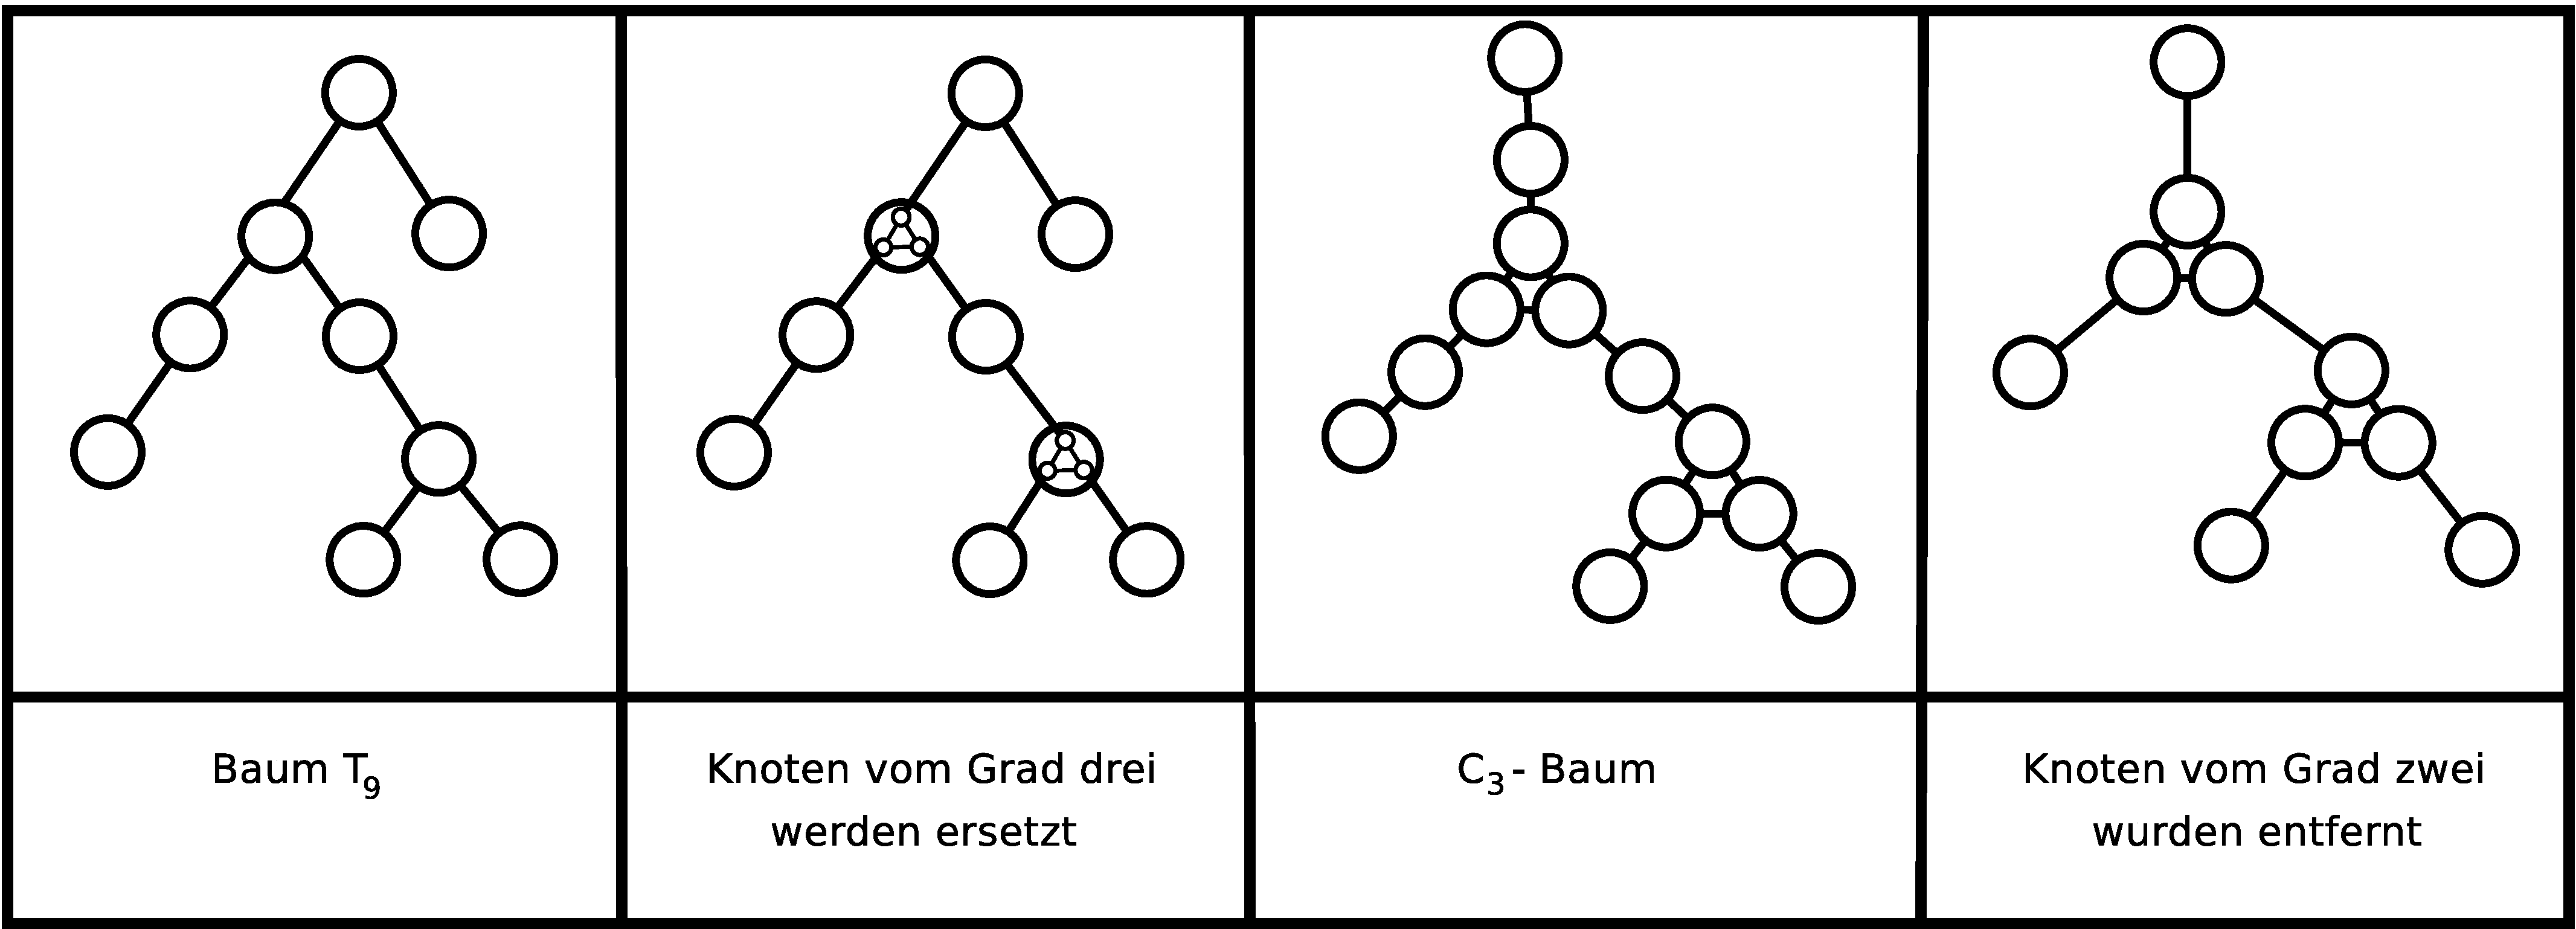
\includegraphics[width=428pt]{bilder/trees.pdf}
	\caption{Entwicklung von einem Baum zum $C_{3}$-Baum}
  	 \end{figure}
\end{bsp}
Gegeben sei der abgebildete Baum $T_9$ mit neun Knoten. Dieser Baum enthält zwei Knoten von Grad drei, welche jeweils wie in der Definition beschrieben durch einen $C_3$ ersetzt werden. Um die Berechnung der metrischen Dimension des enstandenen Graphen zu erleichtern, werden alle Knoten vom Grad zwei kontrahiert.
\begin{lem}
Sei $C_{3,j}$ ein beliebiges $C_{3}$-Blatt. Jede metrische Basis muss mindestens einer der folgenden Knoten $\{v_{j,1},v_{j,2},v_{j,3},v_{j,4}\}$ beinhalten.
\end{lem}
\begin{proof}[Beweis:]~
\par
\vspace{-2mm}
\begin{floatingfigure}[l]{200pt}
{\flushleft
\hspace*{1.7cm}
\includegraphics[width=100pt]{bilder/beweis.pdf}}
\caption{Ein markiertes $C_{3}$-Blatt}
\end{floatingfigure}
Angenommen keiner dieser Knoten ist\\in der metrischen Basis. Durch die eindeutige Verbindung zu dem Restgraphen, welche über einen Trennungsknoten läuft, folgt aus\\Symmetriegründen dass die Knoten $v_{j,3}$ und $v_{j,4}$, sowie $v_{j,1}$ und $v_{j,2}$ identische Markierungen haben.\\Dies ist ein Widerspruch zu der Definition einer metrischen Basis.\\
Damit ist die metrische Dimension eines Graphen $G$ mit mindestens zwei $C_{3,j}$\\mindestens gleich der Anzahl von seinen $C_{3}$-Blätter.
\end{proof}
\par
\vspace{+3mm}
\begin{lem}
Die metrische Dimension (MD) eines Graphen $G$ mit mindestens zwei $C_{3,j}$ ist nicht größer als die Anzahl seiner $C_{3}$-Blätter. 
\end{lem}
%Um diese Eigenschaft zu beweisen werden zwei Sätze über die Struktur solcher $C_{3}-$$Bäume$ benötigt.
\begin{lem}
\label{bkb}
Jeder Knoten eines $C_{3}$-Baumes, welcher kein Blatt ist, ist ein Trennungsknoten.
\end{lem}


\begin{proof}[Beweis:]
Angenommen es gibt einen Knoten $u$, welcher kein Blatt ist und kein Trenunngsknoten. Da der Graph nur aus Knoten von Grad drei und Grad eins besteht ist der Knotengrad von $u$ drei. Dies bedeutet $u$ hat genau drei Nachbaren $v,w,x$. Da der Knoten $u$ nach Annahme kein Trennungsknoten ist, gibt es einen Weg zwischen jedem Paar seiner Nachbarknoten.
\begin{itemize}
\item Fall I: Ein Nachbarknoten ist ein Blatt.\\ Es kommt direkt zum Widerspruch, da durch das Löschen von $u$ sich der Knotengrad des Blattes um eins verkleinert und damit null wird, also $u$ ein getrennter einzelner Knoten ist.
\item Fall II: Alle Nachbarknoten haben den Grad drei.\\
Es muss einen Weg zwischen jedem Knotenpaar geben damit der Graph zusammenhängend ist. Somit gibt es auch einen Weg über alle drei Knoten. Sei der Anfangsknoten von diesem Weg o.B.d.A. der Knoten $v$, der Endknoten o.B.d.A. der Knoten $x$ und der Weg geht über den Knoten $w$. Die Länge dieses Weges ist folgend mindestens drei. Wird wieder der entfernte Knoten $u$ betrachtet welcher zuvor mit allen drei Knoten verbunden war, so folgt, dass der Graph einen Kreis beinhaltet welcher aus dem Weg von $v$ zu $x$ über $w$ besteht und über den entfernten Knoten $u$ zurück zum Knoten $v$ geht.\\
Damit gibt es in dem Graphen mind. einen Kreis mit einer echt größeren Länge als drei und dies ist ein Widerspruch zur Definition des $C_{3}$-Baumes, welche nur Kreise der Länge drei erlaubt.
\end{itemize}
\end{proof}
\begin{lem}
\label{bkb2}
In jedem Teilgraphen eines $C_{3}$-Baumes mit mindestens vier Knoten ist mindestens ein Knoten aus der metrischen Basis.
\end{lem}
\begin{proof}[Beweis:]
Der kleinste Teilgraph der durch das Löschen eines Knotens entstehen kann ist ein Blatt. Dieser besteht allerdings nur aus einem Knoten. Der nächstgrößere Teilgraph der durch das Löschen eines Knotens entstehen kann beinhaltet vier Knoten, genauer den unteren Teil eines $C_{3}$-Blattes. Damit beinhaltet er auch sein linkes Blatt, welches in die metrische Basis aufgenommen wird. Jeder größere Teilgraph beinhaltet diese vier Knoten. %Unabhängig davon welcher Knoten als Wurzel verwendet wurde, galt bei dem ursprünglichen Baum dass der Knoten mit der weitesten Entfernung von der Wurzel(der Knoten davor), hatte genau zwei Kinder und aus dem wurde ein $C_{3,j}-$$Blatt$.  
\end{proof}
\begin{proof}[Beweis von Lemma 27:]
Der gesamte Graph besteht nur aus Knoten vom Grad drei oder Grad eins. In die metrische Basis wird das linke Blatt von jedem $C_{3}$-Blatt aufgenommen. Sei $n$ die Anzahl der $C_{3}$-Blätter und $m$ die Anzahl der $C_{3,j}$, die keine $C_{3}$-Blätter sind und bei diesem Beweis als einfache $C_{3,j}$ bezeichnet werden.
\begin{itemize}
\item Fall I. Die Knoten $u$ und $v$ haben unterschiedliche Distanzen vom Knoten $r_1$ aus der metrischen Basis. Der Knoten $r_1$ trennt die Knoten $u$ und $v$.
\item Fall II. Die Knoten $u$ und $v$ haben die gleiche Distanz vom Knoten $r_1$ aus der metrischen Basis und die Knoten $u$ und $v$ liegen im selben $C_{3,j}$.\\
O.B.d.A. sei $b_1$ der ausgewählte Knoten $r_1$ oder $b_1$ auf allen kürzesten Wegen des Knotens $r_1$ zu jedem Knoten in dem $C_{3,j}$. Es gibt zwei nicht getrennte Knotenpaare durch den Knoten $r_1$, das Knotenpaar $\{b_2,b_3\}$ oder das Knotenpaar $\{c_2,c_3\}$.\\
Angenommen $b_2$ und $b_3$ sind Blätter (daraus folgt das $b_1$ kein Blatt sein kann), so wird o.B.d.A. $b_3$ in die metrische Basis aufgenommen und so ist seine Markierung o.B.d.A. an der ersten Position $0$ und er ist der einzige Knoten mit dieser Markierung. Sein einziger Nachbar $c_3$, bekommt die Markierung $1$ an der ersten Position, damit ist dieser Knoten auch eindeutig markiert. Die anderen zwei Knoten $c_1$ und $c_2$ auf dem $C_3$ bekommen die Markierung $2$ an der ersten Position und ihre zwei Nachbaren $b_1$ und $b_2$, die Markierung $3$ an der ersten Position. Somit kriegen die Knotenpaare $b_2$ und $b_3$ und $c_2$ und $c_3$ unterschiedliche Markierungen und sind getrennt.\\ 	 
Sei nun $b_3$ kein Blatt, damit ist er Teil eines anderen $C_{3,j}$, welcher zwei $C_{3,j}$-Kinder besitzt. Sind beide $C_{3,j}$- Kinder keine Blätter, so sind sie Teile eines anderen $C_{3,j}$. Damit ist $b_3$ nach Lemma \ref{bkb} ein Trennungsknoten. Der Graph ohne die Knoten $b_1$ und $b_2$ beinhaltet mindestens vier Knoten, die anderen Knoten auf diesem $C_{3,j}$ und ihre zwei $C_{3,j}$- Kinder und nach Lemma \ref{bkb2} mindestens ein Element aus der metrischen Basis.\\
Da der Knoten $b_3$ ein Trennungsknoten ist, ist die Distanz von diesem Knoten zu $b_3$ ist echt kleiner als zu jedem anderen Knoten in dem ausgewählten $C_{3,j}$. Die Markierung von $b_3$ sei o.B.d.A. an der ersten Position $a$. Sein einziger Nachbar $c_3$ bekommt die Markierung $a+1$ an der ersten Position. Die anderen zwei Knoten $c_1$ und $c_2$ auf dem $C_3$ bekommen die Markierung $a+2$ an der ersten Position und ihre zwei Nachbaren $b_1$ und $b_2$, die Markierung $a+3$ an der ersten Position. Somit erhalten die Knotenpaare $b_2$ und $b_3$ und $c_2$ und $c_3$ unterschiedliche Markierungen und sind getrennt.
\begin{figure}[h!]
		\centering
 		 \includegraphics[width=400pt]{bilder/bew2.pdf}
   \caption{Ein Graph mit einem ausgesuchten $C_{3,j}$ und festen $r_1$, $r_2$ und $r_3$}
  	 \end{figure}

\item Fall III. Die Knoten $u$ und $v$ haben die gleiche Distanz vom Knoten $r_1$ aus der metrischen Basis und die Knoten $u$ und $v$ liegen in unterschiedlichen $C_{3,j}$.\\
Der Knoten $u$ hat entweder den Grad eins und ist ein Blatt, welches ein Nachbar eines $C_3$ ist, oder den Grad drei und ist Teil eines festen $C_{3}$. Da der Graph zusammenhängend ist, gibt es in beiden Fällen eine Kante $\{x,y\}$ in dem gleichen $C_{3,j}$ mit der Eigenschaft $x$ Teil von diesem $C_{3}$, $y$ nicht und $dist(v,y) < dist(v,x)$. Durch die zweite Anforderung kann $y$ kein Blatt sein. Nach Lemma \ref{bkb} sind $x$ und $y$ zwei Trennungsknoten, und die beiden nicht zusammenhängenden Graphen, welche durch das Entfernen des jeweiligen Knoten entstehen, beinhalten nach Lemma \ref{bkb2} mindestens ein Element aus der metrischen Basis.\\
Der Teilgraph $G_L$ links von der Kante $\{x,y\}$ beinhaltet den Knoten $u$ und mindestens einen Knoten aus der metrischen Basis $r_3$, der Teilgraph $G_R$ an der anderen Seite der Kante $\{x,y\}$ beinhaltet den Knoten $v$ und mindestens einen Knoten aus der metrischen Basis $r_2$. Nach Lemma \ref{first_theorem} sind die Knoten $u$ und $v$ getrennt.
\end{itemize}
\end{proof}
\begin{lem} ~
\begin{enumerate}
\item Fall: Der Baum besteht nur aus Knoten mit $deg(v) \leq 2$. Damit ist dieser Baum ein Weg und seine metrische Dimension ist eins.\\
\item Fall: Der Baum beinhaltet genau einen Knoten mit $deg(v)=3$. Seine metrische Dimension ist zwei.
\end{enumerate}
\end{lem}

%%%%%%%%%%%%%%%%%%%%%%%%%%%%%%%%%%%%%%%%%%%%%%%%%%%%%%%%%%%%%%%%%%%%%%%%%%%%%%%%%%%%%%%%%%%%%%%%%%%%%%%%%%%%%%%%
\section{Verallgemeinerungen}
Unterschiedliche Möglichkeiten sind für die Verallgemeinerung von $C_3-$Bäumen möglich. Einerseits ist es möglich die Kreisordnung zu erhöhen. Eine andere Möglichkeit ist es jeden Knoten durch einen Kreis, dessen Größe mindestens der Ordnung des ersetzten Knotens entspricht, zu ersetzen.

\begin{defi}
Sei ein Baum $T=(V,E)$ mit $deg(v_i)\leq j$ für $v_i \in V$ gegeben. Der $C_j$-Baum resultiert daraus folgend: 
Für alle $3 \leq i \leq j$ und $i \in \mathbb{N}$ sei $$V'=\{v_k|v_k \in V \wedge deg(v_k)=i\}\subseteq V$$ eine Teilmenge der Knoten aus dem Graphen $T$. Ersetze jeden Knoten $v_n \in V'$ durch einen $C_k$ mit $k \geq i$ (bezeichnet wird dieser Teilgraph als \emph{$C_{k,i,n}$}), so dass höchstens ein Knoten von $C_{k,i,n}$ mit genau einem Nachbarn von $v_n$ verbunden ist. Die $i$ Nachbarn von $C_{k,i,n}$ werden als \emph{$C_{k,i}$- Kinder} bezeichnet. Sofern zwei dieser $C_{k,i}$- Kinder Blätter sind wird der Teilgraph, welcher den $C_{k,i,n}$ und seine Nachbarn beinhaltet, als \emph{$C_{k,i}$-Blatt} bezeichnet.
\end{defi}

\begin{bsp}
In der Abbildung \ref{c_jbaum} werden drei Knoten von dem Baum durch Kreise ersetzt. Der rechte Knoten wird durch einen Kreis ersetzt, wobei die Ordnung des Kreises gleich der Anzahl seiner Nachbaren ist. Die zwei anderen Kreise haben mehr Knoten, als Nachbaren, so dass jeweils ein Knoten nur Nachbaren im Kreis hat. Die Ankerknoten wurden im Baum und im $C_j$-Baum eingezeichnet.\\
\vspace{-4mm}
\begin{figure}[h!]
		\centering 		 
   \includegraphics[width=410pt]{bilder/trees3.pdf}
	\caption{Entwicklung von einem Baum zum $C_{j}$-Baum}
	\label{c_jbaum}
  	 \end{figure}
\vspace{-4mm}
\end{bsp}
\begin{bem}
Da ein $C_j$-Baum ein vereinfachter Kaktusgraph ist, kann die metrische Dimension von $C_j$-Bäumen mit einer vereinfachten Variante vom Algorithmus zur Berechnung der MD von Kaktusgraphen berechnet werden.
\begin{algorithm}
\caption{Aufbau vom Algorithmus zur Berechnung der MD von $C_j$-Bäumen}
\begin{algorithmic}
\STATE 1. Bestimme alle zweifachen Zusammenhangskomponente mit mindestens 3 Kanten und\\$\;\;\;\;$ordne jeden Knoten jeder Zusammenhangskomponente zu einer der drei Klassen\\$\;\;\;\;\{0,i,A\}$ mit $i \geq 1$;
\STATE 2. Berechne die metrische Dimension der ZZK vom Typ $S$ und $US$ und ersetze die\\$\;\;\;\;$Komponente durch Bäume;
\STATE 3. Berechne die metrische Dimension des Baumes;
\end{algorithmic}
\end{algorithm}
~\linebreak
Da alle Knoten in einem $C_j$-Baum maximal den Grad drei haben gibt es keine Amalgamationsknoten. Außerdem gibt es in $C_j$-Bäumen keine Kreise, sondern nur vollständige und unvollständige Sonnen.
\end{bem}
%%%%%%%%%%%%%%%%%%%%%%%%%%%%%%%%%%%%%%%%%%%%%%%%%%%%%%%%%%%%%%%%%%%%%%%%%%%%%%%%%%%%%%%%%%%%%%%%%%%%%%%%%%%%%%%%
\section{Vergleich der MD zwischen Bäumen und $C_j$-Bäumen}
Bei $C_3$-Bäumen war die metrische Dimension gleich der metrischen Dimension vom Baum. In der Abbildung \ref{c_jbaum} ist die metrische Dimension deutlich kleiner bei dem $C_j$-Baumen. In dem folgenden Beispiel sind zwei Graphenpaare dargestellt. Bei dem einen ist die metrische Dimension vom Baum zwei und von dem entsprechenden $C_j$-Baum parameterabhängig und bei dem Anderen umgekehrt.\\
\begin{bsp} (a) Sei ein Baum $G=(V,E)$ mit $|V|=2nk+2$ wie in Abbildung \ref{c_jbaum} gegeben.

\begin{figure}[ht]
\centering
\includegraphics*[width = 420pt]{bilder/bspcjbaum3.pdf}
\caption{MD vom $C_j$-Baum ist kleiner als vom Baum}
\label{cjbaum}
\end{figure}
\vspace{-5mm}
~\linebreak
Der Graph besteht aus $k$ Knoten mit $k\geq 3$ auf einem Pfad. Zwei Knoten sind Vorgänger von $2n$ Blättern mit $n\geq 2$ und $k-2$ Knoten sind Vorgänger von jeweils $2n-1$ Blättern. Die metrische Dimension dieses Baumes ist $2nk+2n-2k+2$.\\
Bei dem $C_j$-Baum wurden alle Knoten durch $C_{4n+1}$ ersetzt. Dabei bleiben $2n$ Knoten ohne Blätter und die zwei Nachbarknoten werden mit jeweils einer Kante mit einem weiteren $C_j$ verbunden. Die Distanz von diesen Knoten ist $2n$. Nach Lemma \ref{usg} benötigt ein solcher Teilgraph keine weiteren Ankerknoten. Beide Knoten außen werden durch jeweils einen $C_{2n+1}$ ersetzt und jeder Nachbar von dem ursprünglichen Knoten wird mit genau einem Knoten auf dem Kreis verbunden. Dieser Teilgraph benötigt nach Lemma \ref{usg} einen Ankerknoten. Die metrische Dimension des enstandenen $C_j$-Baumes ist zwei.\newline\newline
(b) Sei der Baum $G=(V,E)$ mit $2k+2$ Knoten und $k\geq 2$ wie in Abbildung \ref{baumcj} gegeben.
\begin{figure}[ht]
\centering
\includegraphics*[width = 420pt]{bilder/bspbaumcj3.pdf}
\caption{MD vom Baum ist kleiner als vom $C_j$-Baum}
\label{baumcj}
\end{figure}
\vspace{-3mm}
~\linebreak
Die metrischer Dimension ist zwei. Der $C_j$-Baum ensteht durch das Ersetzen von Knoten mit Grad drei durch den $C_6$. Verbinde drei nebeneinanderliegende Knoten auf dem Kreis mit den Nachbarn des ursprünglichen Knotens, so dass die Blätter oder das Blatt immer außen ist. Der $C_6$-Baum hat $7k+2$ Knoten und seine metrische Dimension ist $k+2$. Ohne die $k$ zusätzlichen Ankerknoten wären die rotmarkierten Knoten in Abbildung \ref{baumcj} paarweise nicht getrennt.
\end{bsp}
%%%%%%%%%%%%%%%%%%%%%%%%%%%%%%%%%%%%%%%%%%%%%%%%%%%%%%%%%%%%%%%%%%%%%%%%%%%%%%%%%%%%%%%%%%%%%%%%%%%%%%%%%%%%%%%%
%%%%%%%%%%%%%%%%%%%%%%%%%%%%%%%%%%%%%%%%%%%%%%%%%%%%%%%%%%%%%%%%%%%%%%%%%%%%%%%%%%%%%%%%%%%%%%%%%%%%%%%%%%%%%%%%
%%%%%%%%%%%%%%%%%%%%%%%%%%%%%%%%%%%%%%%%%%%%%%%%%%%%%%%%%%%%%%%%%%%%%%%%%%%%%%%%%%%%%%%%%%%%%%%%%%%%%%%%%%%%%%%%
%%%%%%%%%%%%%%%%%%%%%%%%%%%%%%%%%%%%%%%%%%%%%%%%%%%%%%%%%%%%%%%%%%%%%%%%%%%%%%%%%%%%%%%%%%%%%%%%%%%%%%%%%%%%%%%%
\chapter{Zusammenfassung}
\vspace{-5mm}
In dieser Arbeit wurde unter anderem ein Linearzeit-Algorithmus zur Berechnung der metrischen Dimension für Kaktusgraphen entwickelt. Damit wurden die Graphen mit algorithmisch bestimmbarer metrischer Dimension in der Komplexitätslasse \textbf{Lin} erweitert.\vspace{-1.5mm}\newline\newline
Durch die eingeschränkte Struktur von Kaktusgraphen ist es möglich die Berechnung der metrischen Dimension des gesamten Graphen in Teilgraphen aufzuteilen, welche über die Trennungsknoten entstehen. Es konnte gezeigt werden, dass ein Trennungsknoten als Ankerknoten in einem Teilgraphen aufgefasst werden kann, sofern der andere Teilgraph kein Weg ist. Ist ein Teilgraph ein Weg so wird er nicht getrennt betrachtet, sondern zusammen mit dem anderen Teilgraph als ein Sonnengraph.\newline Weiterhin werden die Nachbarschaften der Trennungsknoten untersucht, welche durch eine Graphklasse, die Freundschaftsgraphen, als kleinstes Beispiel simuliert werden konnte. Es wurde bewiesen, dass nur die Nachbarschaften von Trennungsknoten untersucht werden müssen um die Trennung des gesamten Graphen zu gewährleisten. \vspace{-1.5mm}\newline\newline
Die beiden Graphklassen wurden in dem Kapitel zuvor untersucht. Außerdem wurde eine weitere Graphklasse, die $C_j$-Bäume, eingeführt, dessen metrische Dimension mit Hilfe des Algorithmus berechnet werden kann.
\vspace{-5mm}
\section{Ähnliche Arbeiten}
\vspace{-3mm}
\subsection{Andere Dimensionen von Graphen}
\vspace{-2mm}
Insbesondere in den letzten zwei Dekaden wurde intensiv an der Thematik geforscht und zahlreiche Abwandlungen des Problems eingefüht, so u.A. die Oberdimension, die trennende Zahl und die Partitionsdimension.\newline
Die ersten beiden wurden in "Resolvability and the upper dimension of graphs" \cite{upper} eingeführt. Die Oberdimension eines Graphen ist die größte Menge an Knoten, so dass kein Knoten überflüssig ist und die Menge eine trennende Menge ist. Die trennende Zahl ist die Größe der kleinsten Menge an Knoten, so dass bei beliebiger Wahl von Knoten aus dem Graphen, jede Menge dieser Größe eine trennende Menge ist. Sie zu kennen ist nützlich bei Algorithmen, da aus einer Anzahl der Knoten geschlossen werden kann, dass der Graph getrennt ist, ohne die Position der Knoten zu kennen.
\vspace{-1.5mm}\newline\newline 
In der Arbeit "On the partition dimension of a graph" \cite{partit} wurde aus der metrischen Dimension die Partitionsdimension (PD) entwickelt. Während bei der metrischen Dimension nur einzelne Knoten in die Basis aufgenommen werden, dürfen bei der PD Mengen von Knoten aufgenommen werden. Weiterhin muss die gesuchte Partition jeden Knoten trennen und den gesamten Graphen in Mengen aufteilen. Die PD des Graphen $pd(G)$ ist die kleinste Anzahl von Mengen. Die Distanz eines Knotens zu einer Menge ist immer die kürzeste Distanz zu einem Knoten aus der Menge.\newline
Die metrische Dimension um eins erhöht ist eine obere Schranke für die PD\cite{partit}. Es gibt aber auch Graphen mit deutlich kleinerer PD als metrischer Dimension, z.B. den Graphen aus der Arbeit "Discrepancies between metric dimension and partition dimension of a connected graph" \cite{disc}. Viele Fragestellungen sind bereits gelöst worden, aber einige Berechnungen sind noch offen, wie z.B. die Bestimmung der PD bei Bäumen. Es gibt außerdem viele Abwandlungen der PD, z.B. zusammenhängende PD aus "Connected partition dimensions of graphs" \cite{con}, die "Locating-Chromatic Number" aus "The locating-chromatic number of a graph" \cite{loc} und die "Forcing" Dimension aus "The forcing dimension of a graph" \cite{forcing}.
\vspace{-4mm}
\subsection{Algorithmen zur Berechnung der metrischen Dimension}
\vspace{-2mm}
Die Autoren von der Arbeit "On the Complexity of Metric Dimension" \cite{aussenplanar} geben einen Algorithmus zur Bestimmung der metrischen Dimension von einem außenplanaren Graphen in Polynomialzeit an. Der Algorithmus arbeitet mit dem verallgemeinertem Dualbaum des Graphen und überprüft mittels dynamischer Programmierung bestimmte Eigenschaften von Teilbäumen. 
\vspace{-1mm}
\newline\newline
Die metrische Dimension von blätterlosen und nicht antipodalen Block-Kaktusgraphen wird in der Arbeit "Metric Dimension of antipodal and pendant-free block-cactus graphs" \cite{cactusblock} analysiert. Die Kaktusgraphen werden durch vollständige Graphen zusätzlich zu Kreisen erweitert, aber auch starkt eingeschränkt, in dem Wege und Bäume an Kreisknoten verboten werden. In geraden Kreisen werden gegenüberliegende Trennungsknoten nicht erlaubt. Dadurch gibt es noch weniger Fallunterscheidungen. Insbesondere werden in der Arbeit nur Anforderungen an die Anzahl der Ankerknoten in bestimmten Teilgraphen gestellt.
\vspace{-5mm}
\section{Offene Fragen und zukünftige Forschung}
\vspace{-2mm}
Der Algorithmus zur Berechnung der metrischen Dimension von Kaktusgraphen könnte durch das Zulassen von vollständigen Graphen, Gittern, vollständig biparteten Graphen oder auch Radgraphen als zweifache Zusammenhangskomponenten erweitert werden. Dafür müsste die metrische Dimension von diesen Graphen mit Wegen erforscht werden.\\ Die Gittergraphen mit Wegen der Länge eins an den Knoten wurden in "Corrections to the article: The metric dimension of graph with pendant edges" \cite{grid} erforscht, die metrische Dimension von solchen Graphen ist drei. Es ist hier notwendig zunächst das Ergebnis auf beliebige Wege zu erweitern und dann die Graphen zu finden, welche mit Wegen versehen sind, aber noch die metrische Dimension zwei haben. Die anderen Graphen erfordern eine detailierte Untersuchung.
\vspace{-1.5mm}\newline\newline
Ein denkbares Ziel wäre die Erweiterung des Linearzeit-Algorithmus auf außenplanare Graphen. Dazu würden zunächst alle möglichen zweifachen Zusammenhangskomponenten mit Brücken analysiert werden, so wie die Auswirkungen von Komponenten über zwei Knoten aufeinander. Ein Anfang wären die maximalen außenplanaren Graphen, da es weniger unterschiedliche Fälle gibt.
\vspace{-1.5mm}\newline\newline
Außer der Frage in wie weit sich die Linearzeit-Algorithmen erweitern lassen, ist die genaue Zuordnung der Berechnung der metrischen Dimension von Halin-Graphen aus "{Studies on minimally n-connected graphs}" \cite{halin} noch offen. An einem Algorithmus in Polynomialzeit oder einem Beweis der NP-Vollständigkeit könnte geforscht werden.

%%%%%%%%%%%%%%%%%%%%%%%%%%%%%%%%%%%%%%%%%%%%%%%%%%%%%%%%%%%%%%%%%%%%%%%%%%
%%%%%%%%%%%%%%%%%%%%%%%%%%%%%%% ENDE TEXTTEIL %%%%%%%%%%%%%%%%%%%%%%%%%%%%
%%%%%%%%%%%%%%%%%%%%%%%%%%%%%%%%%%%%%%%%%%%%%%%%%%%%%%%%%%%%%%%%%%%%%%%%%%

\clearpage
\bibliographystyle{plain}
\bibliography{references}
%\vspace*{\fill}
\clearpage
\listoffigures
\listoftables
%\pagebreak
%\printindex
\end{document}
